\documentclass[11pt,oneside]{book}
\usepackage{fontspec}
\setmainfont{Noto Serif}
\setsansfont{Noto Sans}
\setmonofont{Noto Sans Mono}
\newfontfamily\proseunicodefont{DejaVu Serif}
\usepackage[margin=1in]{geometry}
\usepackage{microtype}
\usepackage{amsmath,amssymb,amsthm,mathtools,bm}
\usepackage{graphicx}
\usepackage{xcolor}
\usepackage{booktabs}
\usepackage{array}
\usepackage{longtable}
\usepackage{enumitem}
\usepackage{float}
\usepackage{caption}
\usepackage{hyperref}
\usepackage{fancyhdr}
\usepackage{tikz}
\usetikzlibrary{arrows.meta,positioning,calc,decorations.pathmorphing}

\hypersetup{
  colorlinks=true,
  linkcolor=blue!50!black,
  urlcolor=blue!50!black,
  citecolor=blue!50!black
}

\setlength{\parskip}{0.5em}
\setlength{\parindent}{0pt}
\setlist[itemize]{topsep=0.25em,itemsep=0.2em}
\setlist[enumerate]{topsep=0.25em,itemsep=0.2em}
\setlength{\headheight}{40pt}
\numberwithin{equation}{chapter}

\newtheorem{theorem}{Теорема}[chapter]
\newtheorem{proposition}[theorem]{Утверждение}
\newtheorem{lemma}[theorem]{Лемма}
\newtheorem{corollary}[theorem]{Следствие}
\theoremstyle{definition}
\newtheorem{definition}[theorem]{Определение}
\newtheorem{example}[theorem]{Пример}
\theoremstyle{remark}
\newtheorem{remark}[theorem]{Замечание}

\providecommand{\ket}[1]{\left\lvert#1\right\rangle}
\providecommand{\bra}[1]{\left\langle#1\right\rvert}
\providecommand{\braket}[2]{\left\langle#1\,\middle|\,#2\right\rangle}
\providecommand{\expect}[1]{\left\langle#1\right\rangle}
\newcommand{\lectureoverview}[1]{\paragraph{Обзор.} #1}

\makeatletter
\newcommand{\course@headerfont}{\normalfont\small\itshape}
\newcommand{\course@pagefont}{\normalfont\small}
\newcommand{\course@headerraise}{14pt}
\newlength{\course@headerboxheight}
\setlength{\course@headerboxheight}{\dimexpr\headheight-\course@headerraise-9pt\relax}
\newcommand{\course@leftheadbox}[1]{%
  \raisebox{\course@headerraise}{%
    \parbox[t][\course@headerboxheight][t]{0.82\textwidth}{%
      \raggedright\course@headerfont\strut\MakeUppercase{#1}\strut%
    }%
  }%
}
\newcommand{\course@rightheadbox}[1]{%
  \raisebox{\course@headerraise}{%
    \parbox[t][\course@headerboxheight][t]{0.82\textwidth}{%
      \raggedleft\course@headerfont\strut\MakeUppercase{#1}\strut%
    }%
  }%
}
\renewcommand{\chaptermark}[1]{\markboth{\MakeUppercase{\chaptername\ \thechapter.\ #1}}{}}
\renewcommand{\sectionmark}[1]{\markright{\MakeUppercase{\thesection\hspace{0.4em}#1}}}
\fancyhf{}
\fancyhead[L]{\course@leftheadbox{\leftmark}}
\fancyhead[R]{\course@pagefont\thepage}
\renewcommand{\headrulewidth}{0.5pt}
\pagestyle{fancy}
\fancypagestyle{plain}{%
  \fancyhf{}
  \fancyhead[L]{\course@leftheadbox{\leftmark}}
  \fancyhead[R]{\course@pagefont\thepage}
  \renewcommand{\headrulewidth}{0.5pt}
}
\makeatother

% Video2Book editorial provenance macros
\newenvironment{classroomqa}{%
  \par\medskip\noindent\begin{minipage}{\linewidth}\small\hrule\medskip
}{%
  \medskip\hrule\end{minipage}\par\medskip
}
\newcommand{\audiencequestion}[1]{\noindent\textbf{Вопрос из аудитории.} #1\par\smallskip}
\newcommand{\lecturerresponse}[1]{\noindent\textbf{Ответ.} #1\par}
\newcommand{\lecturetimestamp}[1]{\footnote{Время в лекции: #1.}}
\newcommand{\lectureframe}[1]{\par\smallskip{\centering\footnotesize\itshape Кадр лекции: #1.\par}}
\newcommand{\editorialnote}[1]{\footnote{Редакторское пояснение: #1}}

\usepackage{polyglossia}
\setdefaultlanguage{russian}
\usepackage{sectsty}
\renewcommand{\contentsname}{Содержание}
\renewcommand{\chaptername}{Глава}
\renewcommand{\figurename}{Рисунок}
\renewcommand{\tablename}{Таблица}
\renewcommand{\proofname}{Доказательство}
\renewcommand{\bibname}{Литература}
\sectionfont{\raggedright}
\subsectionfont{\raggedright}
\makeatletter
\renewcommand{\@pnumwidth}{2.2em}
\renewcommand{\@tocrmarg}{3.2em}
\makeatother
\usepackage{tocloft}
\renewcommand{\cftchapfont}{\small\bfseries}
\renewcommand{\cftchappagefont}{\small\bfseries}
\renewcommand{\cftsecfont}{\small}
\renewcommand{\cftsecpagefont}{\small}
\setlength{\cftsecnumwidth}{3em}
\renewcommand{\cftsubsecfont}{\small}
\renewcommand{\cftsubsecpagefont}{\small}
\setlength{\cftsubsecindent}{4.5em}
\setlength{\cftsubsecnumwidth}{4em}
\emergencystretch=6em
\pdfstringdefDisableCommands{\def\proseunicodefont{}}

\geometry{paperwidth=177.6mm,paperheight=252mm,left=16mm,right=16mm,
 top=18mm,bottom=18mm,includeheadfoot,headheight=28pt,headsep=7mm,footskip=9mm}
\usepackage{scrextend}
\changefontsizes[17pt]{12pt}
\raggedbottom
\renewenvironment{classroomqa}{\par\medskip\begingroup}{\par\endgroup\medskip}
\fancyhf{}
\setlength{\headwidth}{\textwidth}
\fancyhead[L]{\parbox{\textwidth}{\raggedright\fontsize{9}{11}\selectfont\nouppercase{\leftmark}}}
\fancyfoot[C]{\small\thepage}
\renewcommand{\headrulewidth}{0.3pt}
\fancypagestyle{plain}{\fancyhf{}\fancyfoot[C]{\small\thepage}\renewcommand{\headrulewidth}{0pt}}

\graphicspath{{../../../generated_course_notes/supplementary/particle_physics_3_supersymmetry_and_grand_unification/2010_spring/figures/}{../../../generated_course_notes/supplementary/particle_physics_3_supersymmetry_and_grand_unification/2010_spring/assets/}}
\hypersetup{
  pdftitle={Particle Physics 3: Supersymmetry and Grand Unification},
  pdfauthor={Leonard Susskind},
  pdfsubject={Independently edited companion notes for the 2010 Spring lecture course}
}
\begin{document}
\frontmatter
\hypersetup{pageanchor=false}
\begin{titlepage}
\hyphenpenalty=10000\exhyphenpenalty=10000
\thispagestyle{empty}
\begin{tikzpicture}[remember picture,overlay]
  \node[anchor=center,inner sep=0] at (current page.center) {%
    \includegraphics[height=\paperheight,keepaspectratio]{../../../generated_course_notes/supplementary/particle_physics_3_supersymmetry_and_grand_unification/2010_spring/assets/cover-art.png}%
  };
  \node[
    anchor=north west,
    align=left,
    text width=0.78\paperwidth,
    fill=white,
    fill opacity=0.9,
    rounded corners=8pt,
    inner xsep=10pt,
    inner ysep=8pt
  ] at ([xshift=0.08\paperwidth,yshift=-0.06\paperheight]current page.north west) {%
    {\fontsize{30}{33}\selectfont\bfseries\color{black!88} Физика элементарных частиц 3: суперсимметрия и великое объединение\\[0.85em]}
    {\large\color{black!72} Русское издание / весна 2010}
  };
  \node[
    anchor=south west,
    align=left,
    text width=0.68\paperwidth,
    fill=white,
    fill opacity=0.82,
    text opacity=1,
    rounded corners=6pt,
    inner sep=12pt
  ] at ([xshift=0.08\paperwidth,yshift=0.08\paperheight]current page.south west) {%
    {\normalsize\color{black!78} Оригинальные лекции: Leonard Susskind\\[0.35em]}
    {\small\color{black!72} Сопроводительное издание: \href{https://lazying.art}{LazyingArt LLC} / \href{https://github.com/lachlanchen/Video2Book}{Video2Book}}
  };
\end{tikzpicture}
\mbox{}
\end{titlepage}
\hypersetup{pageanchor=true}

\clearpage
\chapter*{Об этих конспектах}
Эти независимо отредактированные сопроводительные конспекты составлены по лекциям Леонарда Сасскинда. Они были восстановлены по машинным расшифровкам, субтитрам и отобранным кадрам с доски, а затем сверены с доступными исходными материалами. Они не являются оригинальной рукописью профессора Сасскинда и не были им ни проверены, ни одобрены.

Издание было подготовлено \href{https://lazying.art}{LazyingArt LLC} с использованием конвейера \href{https://github.com/lachlanchen/Video2Book}{Video2Book} с открытым исходным кодом. Машинные расшифровки по-прежнему доступны отдельно и могут содержать ошибки распознавания. Редакторские уточнения и нетривиальные реконструкции отмечены в сносках.
\clearpage
\tableofcontents
\mainmatter
\chapter{Ренормировка, естественность и проблема иерархии}

\lectureoverview{Центральные идеи этого курса выросли из вопросов, связанных с ренормировкой в Стандартной модели. Поэтому мы начнем с физического смысла ренормировки: устранить степени свободы, которые для рассматриваемого вопроса слишком маломасштабны и слишком быстры, а затем закодировать их эффекты в эффективном описании. Прототипом служит молекула. Затем анализ размерностей переносит ту же логику в скалярную квантовую теорию поля, где она выявляет квадратичную чувствительность скалярной массы, проблему иерархии поля Хиггса, защиту, которой обладают фермионы и калибровочные бозоны, и еще более серьезную проблему энергии вакуума.}

\section{Физика в масштабе поставленного вопроса}

Большинство идей, которые мы будем развивать в этом квартале, возникло из вопросов о ренормировке---иногда это были загадки, иногда полезные наблюдения---в Стандартной модели. Ренормировка соединяет два образа мышления. Первый состоит в том, чтобы удалить из описания структуры на столь малых расстояниях, что они несущественны для задаваемого вопроса. Второй — это анализ размерностей, который часто определяет ответ на коротких расстояниях еще до вычисления какого-либо трудного интеграла.

Такое устранение деталей происходит по всей физике. Если мы хотим понять ядро, можно начать с кварков и квантовой хромодинамики. Вычислив массы и спины протона и нейтрона, а также их эффективные ядерные силы, мы для многих целей можем забыть об их кварковой подструктуре. Движение ядер достаточно медленно, так что нерелятивистская квантовая механика протонов и нейтронов часто оказывается более полезным описанием.

На следующем уровне атомной физике обычно не требуется знать внутреннее устройство ядра. Ядерная физика сообщает нам, какие ядра и изотопы существуют, и задает такие свойства, как масса и электрический заряд. Затем мы начинаем заново с новым набором эффективных элементарных объектов: ядер и электронов. Кварки, протоны и нейтроны не перестали существовать; их эффекты были сжаты в параметры, которыми обладают ядра.

То, сколько именно сохраняется, зависит от следующего вопроса. В атомном расчете может понадобиться масса ядра, потому что она входит в приведенную массу, и, разумеется, нужен заряд, потому что именно он определяет кулоновское поле. Обычно не нужно знать, какой кварк несет какую долю импульса ядра. Существует примерно 90 зарядов элементов, а если учитывать изотопы, разновидностей ядер становится больше. Этот каталог можно принять как входные данные. Электроны, напротив, пока устранить нельзя: именно их движение и образует атомную структуру.

Решив атомную задачу, мы аналогично можем рассматривать атомы как строительные блоки молекул. Причудливый список Сасскинда из атомов печенья, атомов кофе, атомов шоколада и атомов кетчупа подчеркивает серьезную мысль: на каждом уровне начинается новое описание. Как только известны свойства молекул и силы, молекулы можно соединять в более крупные конструкции, напоминающие Tinkertoy, не возвращаясь на каждом шаге к электронной задаче.

Каждый такой переход представляет собой огрубление. Новое описание может быть менее точным в абсолютном смысле, но на своем масштабе оно гораздо полезнее. Квантовая теория поля делает этот вопрос неизбежным, потому что поле имеет моды на всех длинах волн, в том числе сколь угодно коротких. Поэтому мы суммируем эффекты длин волн, слишком коротких, чтобы их разрешить, и заменяем их новыми эффективными параметрами. Эта операция вместе с анализом размерностей и составляет физическое содержание ренормировки.

\section{Молекула как прототип}

Рассмотрим два атома и спросим, как просто описать их относительное движение. Каждый атом содержит тяжелое ядро и облако электронов. Даже протон примерно в 2000 раз тяжелее электрона, а более тяжелые ядра еще сильнее увеличивают разделение масштабов. Полезная картинка — пара шаров для боулинга, окруженных быстро летающими мухами: ядра откликаются медленно, тогда как электронное состояние быстро перестраивается.

Пусть положения и импульсы ядер равны \(R_a\) и \(P_a\), причем оба ядра имеют массу \(M\), а координаты и импульсы электронов — \(r_i\) и \(q_i\), при массе \(m_e\). Опуская стандартные множители, такие как \(4\pi\epsilon_0\), гамильтониан имеет схематический вид
\begin{align}
H={}&
\frac{P_1^2}{2M}+\frac{P_2^2}{2M}
+\frac{e^2}{R_{12}}
+\sum_i\frac{q_i^2}{2m_e}
+\frac12\sum_{i\ne j}\frac{e^2}{r_{ij}}
\nonumber\\
&-\sum_i\left(
\frac{e^2}{|R_1-r_i|}
+\frac{e^2}{|R_2-r_i|}
\right).
\label{eq:molecular-hamiltonian}
\end{align}
Первая строка содержит кинетические энергии ядер, их взаимное кулоновское отталкивание и кинетическую энергию электронов. Вторая включает электрон-электронное отталкивание и электрон-ядерное притяжение. Для ядер с произвольными зарядами восстанавливаются соответствующие множители \(Z_a\); в лекции заряды оставлены схематическими, поскольку существенным здесь является разделение временных масштабов.

Здесь есть два характерных типа движения. Ядра тяжелы и медленны; электроны легки и движутся настолько быстро, что выглядят как размытое пятно. В первом приближении зафиксируем положения ядер и соберем все зависящие от электронов члены в электронный гамильтониан,
\begin{equation}
H_{\mathrm{el}}(R_1,R_2).
\end{equation}
Для каждой фиксированной конфигурации ядер решаем
\begin{equation}
H_{\mathrm{el}}(R_1,R_2)
\psi_0(r_1,\ldots,r_N;R_1,R_2)
=
E_{\mathrm{el}}(R_1,R_2)\psi_0.
\label{eq:electronic-ground-state}
\end{equation}
Мы сохраняем наименьшее электронное собственное значение. Электроны не были отброшены; все их быстрое движение суммировано функцией
\(E_{\mathrm{el}}(R_1,R_2)\).

Логика здесь адиабатическая. За время одной быстрой электронной перестройки ядра смещаются настолько мало, что их координаты можно считать параметрами. После решения электронной задачи на собственные значения этим же координатам снова позволяют изменяться. При каждой медленно меняющейся конфигурации электронное облако следует своему мгновенному основному состоянию. Более точное рассмотрение могло бы сохранить возбужденные электронные поверхности и переходы между ними, но уже ведущая поверхность демонстрирует идею ренормировки.

\begin{figure}[htbp]
\centering
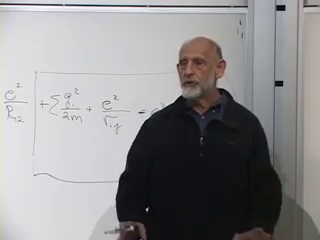
\includegraphics[width=0.72\textwidth]{lecture_01_figure_02.png}
\caption{Молекулярный гамильтониан остается на доске, пока вводится задача об основном состоянии электронной подсистемы. Набранная форма в формуле~\eqref{eq:molecular-hamiltonian} фиксирует члены, скрытые в этом кадре.}
\lectureframe{00:16:19}
\end{figure}

\begin{classroomqa}
\audiencequestion{Ядерные импульсы просто приравниваются нулю?\lecturetimestamp{00:15:39}}
\lecturerresponse{Только временно. В ведущем приближении ядра считаются как бы жестко закрепленными, потому что они движутся намного медленнее электронов. Их импульсы будут восстановлены, когда мы будем решать эффективную задачу для ядер, так что это приближение не нарушает принцип неопределенности.}
\end{classroomqa}

Энергия основного электронного состояния теперь дает вклад в потенциал, который ощущают ядра:
\begin{equation}
V_{\mathrm{eff}}(R_1,R_2)
=\frac{e^2}{R_{12}}+E_{\mathrm{el}}(R_1,R_2).
\label{eq:molecular-effective-potential}
\end{equation}
Для двух изолированных атомов вращательная и трансляционная инвариантность сводят его к функции от расстояния между ними \(R_{12}\). На очень малых расстояниях доминирует кулоновское отталкивание ядер. На очень больших расстояниях взаимодействие слабо. Между этими пределами электронное облако может создать область притяжения и минимум. Тогда волновая функция ядер локализуется вблизи этого минимума и описывает связанную молекулу.

Обратите внимание на порядок действий. Мы не угадывали эмпирическое притяжение и не выбрасывали электроны. Сначала мы решили их квантовую задачу на фиксированном ядерном фоне. Лишь затем мы стерли их явные координаты и сохранили полученное собственное значение. Физика коротких расстояний сохраняется в форме, глубине и кривизне \(V_{\mathrm{eff}}\). Положение его минимума задает равновесное расстояние, его кривизна управляет малыми колебаниями, а его асимптотическая форма определяет, существует ли связанное состояние. Одна эффективная функция переносит всю эту электронную информацию в более медленную задачу.

Таким образом, сложный многоэлектронный гамильтониан превратился в двухчастичный гамильтониан ядер с новым потенциалом. Мы устранили быстрые степени свободы, но сохранили весь их низкоэнергетический эффект. Потенциал ренормирован. Это знакомое рассуждение Борна--Оппенгеймера обычно не вводят под таким названием, однако в нем содержится в точности нужная нам идея:
\begin{equation}
\begin{gathered}
\text{fast microscopic dynamics}\\
\Downarrow\\
\text{effective parameters for slow dynamics}
\end{gathered}
\end{equation}

\section{Естественные единицы и размерность поля}

В квантовой теории поля устраняемые моды можно равносильно описывать как моды коротких расстояний, коротких длин волн, высоких частот или высоких энергий. Прежде чем рисовать диаграммы, зафиксируем учет размерностей.

В обычной механике используются независимые единицы длины, времени и массы. В физике элементарных частиц полагают
\begin{equation}
\hbar=c=1.
\end{equation}
Тогда энергия и масса эквивалентны благодаря \(E=mc^2\), длина и время эквивалентны, потому что \(c=1\), а благодаря \(\hbar=1\) импульс имеет размерность обратной длины. Остается только одна размерность:
\begin{equation}
[M]=[E]=[p]=L^{-1},
\qquad
[x]=[t]=L.
\label{eq:natural-units}
\end{equation}

Это не отменяет размерностей. Просто выбираются коэффициенты пересчета так, что время можно выражать как длину, а массу — как обратную длину. Как только задана одна единица, все остальные определяются автоматически. Поэтому обрезание можно описывать либо как малое расстояние \(\delta\), либо как высокую энергию
\(\Lambda=1/\delta\): это один и тот же масштаб, выраженный на двух языках.

Рассмотрим одно вещественное скалярное поле \(\phi\) со схематически нормированной плотностью лагранжиана
\begin{equation}
\mathcal L=(\partial_\mu\phi)(\partial^\mu\phi)-V(\phi),
\qquad
S=\int d^4x\,\mathcal L.
\label{eq:scalar-action}
\end{equation}

\begin{figure}[htbp]
\centering
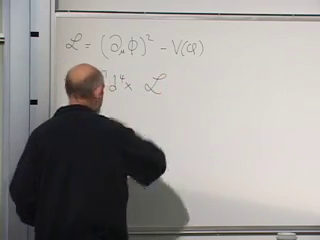
\includegraphics[width=0.78\textwidth]{lecture_01_figure_03.png}
\caption{Локальная скалярная плотность лагранжиана и её интеграл по пространству-времени, образующий действие.}
\lectureframe{00:26:08}
\end{figure}

Плотность лагранжиана локальна: она описывает одну точку пространства-времени. Классические уравнения поля получаются из условия стационарности действия. В квантовой теории то же действие входит в фазу интеграла по траекториям \(\exp(iS)\). В обоих подходах решающей оказывается размерность \(S\). Если восстановить \(\hbar\), фаза имеет вид \(\exp(iS/\hbar)\); после выбора \(\hbar=1\) сама величина \(S\) должна быть безразмерной.

\begin{classroomqa}
\audiencequestion{Имеет ли действие размерность
\(\hbar\)?\lecturetimestamp{00:26:13}}
\lecturerresponse{Да. Поскольку \(\hbar\) положена равной единице, в этих единицах действие безразмерно. Четырёхмерная мера имеет размерность \(L^4\), поэтому плотность лагранжиана должна иметь размерность \(L^{-4}\).}
\end{classroomqa}

Кинетический член теперь фиксирует размерность поля:
\begin{align}
[S]&=1, & [\mathcal L]&=L^{-4},\\
[\partial_\mu]&=L^{-1}, &
[(\partial\phi)^2]&=L^{-2}[\phi]^2=L^{-4},\nonumber\\
&& [\phi]&=L^{-1}.
\label{eq:scalar-dimension}
\end{align}
Этот небольшой расчёт определит ультрафиолетовый порядок величины каждой диаграммы, которая появится далее.

Разложим потенциал в виде
\begin{equation}
V(\phi)=\frac{m^2}{2}\phi^2+g\phi^3+\lambda\phi^4+\cdots.
\label{eq:scalar-potential}
\end{equation}
Каждый член должен иметь размерность \(L^{-4}\). Поскольку
\([\phi^n]=L^{-n}\),
\begin{equation}
[m^2]=L^{-2},
\qquad
[g]=L^{-1},
\qquad
[\lambda]=1.
\label{eq:coupling-dimensions}
\end{equation}
Константа квартического взаимодействия безразмерна. Такие константы связи особенно важны при перенормировке, поскольку их зависимость от масштаба не выводится из простой степени длины.

\begin{classroomqa}
\audiencequestion{Имеет ли \(g\) размерность массы?\lecturetimestamp{00:29:52}}
\lecturerresponse{Да. Множитель \(\phi^3\) имеет размерность \(L^{-3}\), тогда как плотность потенциала должна иметь размерность \(L^{-4}\). Следовательно, \([g]=L^{-1}\), что в естественных единицах соответствует массе.}
\end{classroomqa}

\section{Вершины и пропагатор на коротких расстояниях}

Правила Фейнмана строятся из вершин и пропагаторов. Член \(g\phi^3\) даёт вершину с тремя линиями, которой соответствует множитель, пропорциональный \(g\); \(\lambda\phi^4\) даёт вершину с четырьмя линиями, которой соответствует множитель, пропорциональный \(\lambda\). Квадратичный член даёт локальную двухточечную вставку. Её можно изобразить как частицу, которая входит, поглощается и вновь испускается, с коэффициентом, пропорциональным \(m^2/2\). Численные нормировки, знаки, множители \(i\) и факторы симметрии намеренно опущены, потому что в лекции извлекают зависимость от масштаба, а не вычисляют сечение.

У этих рисунков есть операционное прочтение. Трёхточечная вершина может поглотить два кванта и испустить один, либо представлять любое связанное с кроссингом назначение её трёх линий. Четырёхточечная вершина может описывать две входящие и две выходящие частицы. Квадратичный крестик всё ещё является допустимой двухлинейной вершиной, хотя обычно его включают в свободный пропагатор. Мы изображаем его явно, потому что всякий неразрешённый двухточечный процесс вскоре будет распознаваться сравнением с ним.

Пропагатор соединяет две точки пространства-времени. Его линия не означает, что квантовая частица следовала по прямолинейной классической траектории. Она представляет амплитуду создать возбуждение поля в \(x\) и уничтожить или зарегистрировать его в \(y\):
\begin{equation}
\Delta(x-y)=\langle0|\phi(y)\phi(x)|0\rangle.
\label{eq:position-propagator}
\end{equation}
Читайте это выражение справа налево. Действие \(\phi(x)\) на вакуум создаёт одночастичную компоненту в \(x\). Действие \(\phi(y)\) на бра-вектор уничтожает компоненту в \(y\). Их вакуумный матричный элемент есть амплитуда перекрытия между созданием в первой точке и регистрацией во второй. Символы \(x\) и \(y\) обозначают целые четырёхвекторы, а не только две декартовы координаты.

Состояния не имеют физической размерности, тогда как каждое поле имеет размерность \(L^{-1}\). Следовательно,
\begin{equation}
[\Delta]=L^{-2}.
\end{equation}
Для безмассового поля внутреннего масштаба длины нет, и размерный анализ вынуждает короткодистанционное поведение
\begin{equation}
\Delta(x-y)\sim\frac{1}{(x-y)^2}.
\label{eq:massless-propagator}
\end{equation}
В знаменателе стоит лоренц-инвариантный квадрат интервала, с обычным предписанием, необходимым в его сингулярностях.\editorialnote{Для подсчёта степеней удобно выполнить поворот Вика к евклидову разделению, где величина однозначно пропорциональна \(1/|x-y|^2\). Это не меняет ультрафиолетовые степени, используемые ниже.}

Когда \(y\) приближается к \(x\), пропагатор расходится. Эта сингулярность распространения на исчезающе малом интервале является источником, из которого строятся ультрафиолетовые расходимости в более сложных диаграммах.

\section{Как перенормируется масса скалярного поля}

Для скалярного поля динамическим параметром служит \(m^2\), как уже подсказывает релятивистское дисперсионное соотношение:
\begin{equation}
E=\sqrt{\mathbf p^2+m^2}.
\end{equation}
Пусть \(\delta\) — наименьшее расстояние, которое различает наше эффективное описание. Мы не будем различать процессы, вершины которых разделены расстоянием меньше \(\delta\). Любой такой неразрешённый процесс с одним входящим и одним исходящим скаляром имеет ту же наблюдаемую двухточечную структуру, что и массовая вставка, и потому должен вносить вклад в эффективную массу.

Рассматривайте ускоритель как микроскоп. Если его предельное разрешение равно \(\delta\), то поглощение в одной точке, за которым следует испускание на расстоянии, намного меньшем \(\delta\), нельзя отличить от действительно локального события. Мы намеренно размываем вершину на этом масштабе. Перенормировка — это правило, которое переносит все такие альтернативы ниже предела разрешения в коэффициент соответствующего локального оператора.

\subsection{Первая поправка от квартического взаимодействия}

Начнём с одной вершины \(\phi^4\). Две линии относятся к внешней частице; две другие замыкаются в короткую петлю, испускаемую и вновь поглощаемую почти в одной и той же точке. Если размазать пропагатор в совпадающих точках по расстоянию отсечки, получаем
\begin{equation}
\Delta(0)\ \longrightarrow\ \Delta(\delta)\sim\frac{1}{\delta^2},
\end{equation}
и, следовательно,
\begin{equation}
\delta m^2_{(1)}\sim\frac{\lambda}{\delta^2}.
\label{eq:one-loop-scalar-mass}
\end{equation}
Если \(m_0^2\) обозначает исходный, или голый, параметр, то коэффициент двухточечного члена при низком разрешении схематически имеет вид
\begin{equation}
\frac{m_{\mathrm{eff}}^2}{2}
\sim
\frac{m_0^2}{2}
+c_1\frac{\lambda}{\delta^2},
\label{eq:first-renormalized-mass}
\end{equation}
где \(c_1\) включает в себя опущенные численные и зависящие от соглашений множители. Лабораторная масса, измеряемая в экспериментах, которые не разрешают расстояния меньше \(\delta\), — это именно эта перенормированная величина, а не одно лишь \(m_0\).

Итак, наблюдаемое двухточечное событие может происходить двумя неразличимыми способами. Исходная квадратичная вершина может поглотить и вновь испустить частицу, либо квартическое взаимодействие может сделать то же самое, кратковременно испустив и вновь поглотив виртуальный скаляр. Квантовая механика складывает амплитуды. Как только петля оказывается ниже масштаба разрешения, её отдельная история исчезает из эффективного описания, но её вклад в измеряемый коэффициент — нет.

\subsection{Следующая поправка от квартического взаимодействия}

Теперь соединим две квартические вершины так, чтобы одна внешняя частица входила в \(x\), одна выходила из \(x+\Delta\), а три внутренних пропагатора соединяли вершины. Возникают две степени \(\lambda\), а пропагаторы дают \(\Delta^{-6}\). Квантовые амплитуды нужно просуммировать по всем неразрешённым точкам, из которых может выйти исходящая частица, поэтому интегрирование ведётся по относительному четырёхвектору:
\begin{equation}
\delta m^2_{(2)}
\sim
\lambda^2
\int_{|\Delta|\gtrsim\delta}
d^4\Delta\,\frac{1}{|\Delta|^6}.
\label{eq:two-loop-power-count}
\end{equation}

\begin{classroomqa}
\audiencequestion{Означает ли маленькая метка у вершины, что там есть только три частицы?\lecturetimestamp{00:46:35}}
\lecturerresponse{Нет. Мы по-прежнему используем квартическое взаимодействие. В каждой вершине сходятся четыре линии; в этой двухточечной диаграмме одна линия внешняя, а три идут между двумя вершинами. Во второй вершине снова сходятся четыре линии.}
\end{classroomqa}

Мера даёт четыре степени длины, а три пропагатора — степень минус шесть. Поскольку в этой оценке единственным масштабом служит ультрафиолетовая отсечка,
\begin{equation}
\int_{|\Delta|\gtrsim\delta}
\frac{d^4\Delta}{|\Delta|^6}
\sim\frac{1}{\delta^2},
\qquad
\delta m^2_{(2)}
\sim\frac{\lambda^2}{\delta^2}.
\label{eq:two-loop-scalar-mass}
\end{equation}
Здесь \(\Delta^\mu\) — четырёхкомпонентная переменная интегрирования; интегрирование ведётся по её временной и трём пространственным компонентам. Строчная \(\delta\) обозначает фиксированную отсечку. В лекции сначала для обеих величин употребляется одно и то же произносимое название, а позже обозначения уточняются.

Тот же результат виден, если записать четырёхмерную меру в радиальных координатах. С точностью до углового множителя,
\begin{equation}
\int_{\delta}\frac{d^4\Delta}{|\Delta|^6}
\sim
\int_{\delta}\frac{R^3\,dR}{R^6}
=\int_{\delta}\frac{dR}{R^3}
\sim\frac{1}{\delta^2}.
\end{equation}
Именно поэтому верхний предел на больших расстояниях несуществен для ультрафиолетовой оценки: интеграл определяется своим нижним пределом.

В диаграммах более высокого порядка эта схема повторяется. Диаграмма с большим числом квартических вершин вносит более высокую степень \(\lambda\), но размерный анализ по-прежнему допускает квадратично расходящийся вклад в массу:
\begin{equation}
\begin{aligned}
m_{\mathrm{eff}}^2
={}&m_0^2
+\frac{1}{\delta^2}
\left(c_1\lambda+c_2\lambda^2+c_3\lambda^3+\cdots\right)\\
&+\text{weaker terms}.
\end{aligned}
\label{eq:scalar-mass-series}
\end{equation}

\subsection{Кубическое взаимодействие и логарифм}

Две кубические вершины дают два пропагатора между близкими точками. Их вклад ведёт себя как
\begin{equation}
\delta m_g^2
\sim
g^2\int_{|\Delta|\gtrsim\delta}
\frac{d^4\Delta}{|\Delta|^4}.
\label{eq:cubic-loop}
\end{equation}
Теперь в мере и знаменателе стоят одинаковые степени. Оставшаяся зависимость логарифмическая, а не степенная:
\begin{equation}
\delta m_g^2
\sim
c_g g^2\log\!\left(\frac{1}{\mu\delta}\right).
\label{eq:cubic-log}
\end{equation}
Масштаб сравнения \(\mu\) делает логарифм безразмерным. Это полностью размерная запись схематического \(g^2\log\delta\) из лекции. Логарифм меняется гораздо медленнее любой обратной степени, поэтому при уменьшении длины отсечки доминирует \(1/\delta^2\).

И здесь радиальная форма снова делает различие наглядным:
\begin{equation}
\int_{\delta}^{R_{\mathrm{IR}}}
\frac{d^4\Delta}{|\Delta|^4}
\sim
\int_{\delta}^{R_{\mathrm{IR}}}\frac{R^3\,dR}{R^4}
=\log\!\left(\frac{R_{\mathrm{IR}}}{\delta}\right).
\end{equation}
Равные степени в мере и знаменателе дают логарифм. Большее число степеней в знаменателе даёт обратную степень отсечки. Лекция не требует от нас вычислять угловые множители; она учит нас с первого взгляда распознавать ультрафиолетовый ответ.

\begin{classroomqa}
\audiencequestion{Какое основание у логарифма?\lecturetimestamp{00:57:42}}
\lecturerresponse{Используйте натуральный логарифм. Смена основания лишь умножает его на числовую константу, и эта константа поглощается тем коэффициентом, для которого множители \(2\), \(\pi\) и симметрийные множители здесь не вычислялись.}
\end{classroomqa}

\begin{classroomqa}
\audiencequestion{Как можно брать логарифм от длины и откуда берётся размерность поправки к массе?\lecturetimestamp{00:58:32}}
\lecturerresponse{Логарифм всегда сопоставляет два масштаба; строго говоря, это логарифм безразмерного отношения, такого как \(1/(\mu\delta)\). Константа связи \(g\) имеет размерность массы в первой степени, так что \(g^2\) уже имеет в точности размерность квадрата массы, которая и требуется для этой поправки.}
\end{classroomqa}

\begin{classroomqa}
\audiencequestion{Диаграмма Фейнмана даёт амплитуду. Является ли квадрат её модуля вероятностью?\lecturetimestamp{00:59:41}}
\lecturerresponse{Да, когда амплитуду подставляют в расчёт физического перехода с необходимыми факторами состояний и фазового пространства. Здесь её более непосредственная роль иная: неразрешённая двухточечная амплитуда имеет ту же локальную форму, что и массовый член, и потому сдвигает эффективный параметр массы.}
\end{classroomqa}

\section{Каждый параметр становится эффективным}

Бесконечное семейство массовых диаграмм не исчезает просто потому, что \(\lambda\) мало. Теория возмущений упорядочивает их по степеням константы связи, так что последующие члены могут становиться меньше, но их всё равно бесконечно много. То же исключение короткодистанционных вкладов перенормирует и сами взаимодействия.

\begin{classroomqa}
\audiencequestion{Даже для перенормировки массы разве диаграмм не бесконечно много?\lecturetimestamp{01:00:35}}
\lecturerresponse{Да. Если \(\lambda\) достаточно мало, ряд теории возмущений может быть полезен, потому что всё более высокие степени последовательно подавляются. Тем не менее перенормированный параметр определяется всем рядом, а не одним лишь первым рисунком.}
\end{classroomqa}

Операционально локальное взаимодействие \(\lambda\phi^4\) — это амплитуда процесса с двумя частицами на входе и двумя на выходе. Если более сложный четырёхточечный процесс целиком происходит внутри неразрешаемой области, то при низком разрешении он неотличим от исходной локальной вершины. Поэтому такие диаграммы объединяются в эффективную \(\lambda\). Их ведущая зависимость от масштаба в четырёхмерной теории \(\phi^4\) обычно логарифмическая. В лекции эта бета-функция не вычисляется; этот пример используется, чтобы сформулировать общее утверждение:
\begin{equation}
\begin{gathered}
\text{parameters measured at low energy}\\
\ne\\
\text{parameters entered at the microscopic cutoff}
\end{gathered}
\end{equation}

Этот четырёхточечный пример важен, потому что устраняет возможное недоразумение. Перенормировка — не специальное исправление, применяемое только к расходимости массы. Каждый оператор, допустимый в лагранжиане, может быть воспроизведён неразрешёнными диаграммами с теми же внешними линиями и симметриями. Двухточечный процесс перенормирует коэффициент при квадратичном члене, четырёхточечный процесс перенормирует коэффициент при члене четвёртой степени, а процессы из вакуума в вакуум будут перенормировать постоянный член. Низкоэнергетический лагранжиан — это компактный реестр, в котором записаны все эти короткодистанционные процессы.

\begin{classroomqa}
\audiencequestion{Поскольку \(\Delta\) имеет размерность длины, разве логарифм от неё не выглядит размерностно странно? И разве на доске не перепутали прописную и строчную дельту?\lecturetimestamp{01:01:34}}
\lecturerresponse{Логарифм на самом деле означает отношение к другому масштабу и потому безразмерен. Да, обозначения на мгновение были перепутаны: \(\Delta^\mu\) — переменная интегрирования, а \(\delta\) — нижнее отсечение по расстоянию, которое остаётся в ответе.}
\end{classroomqa}

Это полетеоретический аналог случая с молекулой. Мы решили задачу для ненаблюдаемых быстрых электронов и включили их результат в потенциал. Здесь мы суммируем ненаблюдаемые короткодистанционные процессы и включаем их результат в массы, константы связи и все остальные допустимые локальные коэффициенты. Сдвигается всё.

\begin{classroomqa}
\audiencequestion{Не могли бы вы повторить: включает ли измеряемая величина масштабы, меньшие тех, которые эксперимент способен увидеть?\lecturetimestamp{01:05:13}}
\lecturerresponse{Да, включает. Их отдельные флуктуации не разрешаются, но их суммарный эффект присутствует. Все диаграммы, включающие более короткие масштабы, собираются в один эффективный коэффициент, который низкоэнергетический эксперимент называет, например, физическим квадратом массы.}
\end{classroomqa}

\begin{classroomqa}
\audiencequestion{Должен ли тогда исходный член \(m_0^2\) компенсировать остальные вклады?\lecturetimestamp{01:06:00}}
\lecturerresponse{Если измеряемая масса скаляра намного меньше отдельных ультрафиолетовых вкладов, то да. Требуемая компенсация и есть проблема тонкой настройки, к которой мы теперь переходим.}
\end{classroomqa}

\section{Проблема иерархии Хиггса}

Представьте, что отсечение задаётся планковской длиной, так что от эффективной теории поля требуется суммировать флуктуации от лабораторных масштабов вплоть до масштаба, на котором должна вступить квантовая гравитация.
В единицах физики частиц,
\begin{equation}
\delta\sim M_{\mathrm{Pl}}^{-1}\sim10^{-19}\,\mathrm{GeV}^{-1},
\qquad
\frac{1}{\delta^2}\sim10^{38}\,\mathrm{GeV}^2.
\label{eq:planck-cutoff}
\end{equation}
Точное использование приведённого или неприведённого масштаба Планка несущественно для этого огромного сравнения.

Иерархия расстояний столь же поразительна. Планковская длина примерно на девятнадцать порядков меньше радиуса протона и примерно на шестнадцать или семнадцать порядков меньше расстояний, непосредственно зондируемых обсуждаемыми ускорителями. Именно возведение этого отношения в квадрат превращает большую иерархию длин в компенсацию примерно до 34-го знака после запятой в параметре квадрата массы скаляра.

Для поля Хиггса, скаляра, желаемый слабый масштаб имеет порядок нескольких сотен ГэВ, а не \(10^{19}\) ГэВ. Однако члены в уравнении ~\eqref{eq:scalar-mass-series} естественным образом могут иметь величину планковского масштаба. Их знаки здесь не отслеживались: некоторые могут быть положительными, а некоторые отрицательными, и голый параметр квадрата массы тоже может иметь любой знак. Но чтобы остался остаток электрослабого масштаба, эти огромные части должны сократиться примерно до 34-го знака после запятой. Сначала Susskind говорит о 17 знаках, а затем исправляет себя, потому что сравнение идёт между квадратами масс. Именно квадрат отношения и измеряет эту разновидность тонкой настройки.

\begin{classroomqa}
\audiencequestion{\(\lambda\) меньше или больше единицы?\lecturetimestamp{01:09:50}}
\lecturerresponse{Предполагается, что она умеренно меньше единицы. Теория возмущений стала бы неуправляемой, если бы последовательные степени росли, а чисто скалярную теорию также нельзя согласованно экстраполировать при сколь угодно большой квартической константе связи. Но \(\lambda\) и близко не столь мало, как \(10^{-38}\); для ориентировки в лекции берётся число порядка процентов.}
\end{classroomqa}

\begin{classroomqa}
\audiencequestion{Даже если \(\lambda<1\), разве не остаются важными многие члены, поскольку каждый несёт большой фактор отсечения?\lecturetimestamp{01:10:43}}
\lecturerresponse{Да. Более высокие степени в конце концов подавляют ряд, но до этого заметный вклад может дать большое число членов. Им всем вместе с голым членом пришлось бы согласованно подстроиться, чтобы оставить необычайно малый физический результат.}
\end{classroomqa}

Напомним, почему известно, что параметр массы Хиггса имеет электрослабый масштаб. В обозначениях лекции потенциал нарушения симметрии записывается как
\begin{equation}
V(\phi)=-\frac{\mu^2}{2}\phi^2+\frac{\lambda}{4}\phi^4.
\label{eq:higgs-potential}
\end{equation}
Отрицательный коэффициент при квадратичном члене делает начало координат неустойчивым, тогда как положительный квартический член стабилизирует потенциал. Дифференцирование,
\begin{equation}
\frac{dV}{d\phi}=-\mu^2\phi+\lambda\phi^3
=\phi(-\mu^2+\lambda\phi^2),
\end{equation}
даёт ненулевой минимум
\begin{equation}
\phi_{\min}^2=f^2=\frac{\mu^2}{\lambda}.
\label{eq:higgs-minimum}
\end{equation}
На доске квартический член схематически записан как \(\lambda\phi^4\), но цитируется уравнение ~\eqref{eq:higgs-minimum}; вставка обычного множителя \(1/4\) делает эти две строки согласованными, не меняя аргумента.

Знак \(-\mu^2\) важен, но не спасает естественность. Именно отрицательная кривизна в начале координат приводит к спонтанному нарушению симметрии. Перенормировка сдвигает эту кривизну большими положительными и отрицательными вкладами. Наблюдаемый вакуум с нарушенной симметрией требует, чтобы их сумма была не просто малой, а имела то конкретное малое отрицательное значение, которое помещает минимум на электрослабый масштаб.

Массы бозонов \(W\) и \(Z\) определяют \(f\) как величину порядка \(200\,\mathrm{GeV}\) в грубой нормировке, используемой в лекции. Если \(\lambda\) не является ни огромной, ни фантастически малой, то \(\mu\) должен иметь тот же общий порядок. Следовательно, наблюдаемый коэффициент электрослабого масштаба есть остаток вкладов, каждый из которых может быть на многие десятки порядков больше.

Это называют проблемой тонкой настройки Хиггса, проблемой иерархии или проблемой калибровочной иерархии. Иерархия — это громадное отношение между обычным слабым масштабом и возможным масштабом объединения или планковским масштабом. Малое число само по себе не обязано быть парадоксом. Тревожит здесь то, что малое число собрано из больших, по-видимому не связанных между собой частей, которые должны компенсировать друг друга с чрезвычайной точностью. Эта проблема была осознана в конце 1970-х и начале 1980-х годов, и поиск механизма, стоящего за такой компенсацией, служит мотивацией для суперсимметрии и ряда конкурирующих идей.

Бесконечный ряд теории возмущений не снимает проблему, а лишь обостряет её. \(\lambda\) порядка процентов делает достаточно высокие степени малыми, но прежде чем это подавление начнёт преобладать, может накопиться много членов. Недостаточно, чтобы однопетлевой вклад случайно сократил голую массу. Эффективный слабый масштаб должен оставаться устойчивым и после учёта остальных короткодистанционных процессов. Объяснением было бы структурное соотношение между членами; несвязанная компенсация цифра за цифрой — всего лишь подстройка.

\section{Почему масса фермиона ведёт себя лучше}

Другие частицы Стандартной модели не требуют независимых подстроек того же рода. Для дираковского фермиона массовый член имеет вид
\begin{equation}
\mathcal L_m=-m\bar\psi\psi
=-m\left(\bar\psi_L\psi_R+\bar\psi_R\psi_L\right).
\label{eq:fermion-mass}
\end{equation}
Он содержит саму массу, а не её квадрат, и связывает левую и правую хиральности. Поэтому локальная массовая вставка переводит \(L\) в \(R\) или \(R\) в \(L\).

\begin{figure}[htbp]
\centering
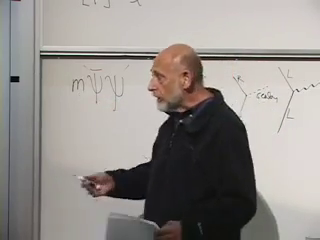
\includegraphics[width=0.76\textwidth]{lecture_01_figure_04.png}
\caption{Фермионный массовый член и нарисованные на доске схематические линии, меняющие хиральность. Ниже диаграммы восстановлены алгебраически, поскольку часть мелового рисунка заслонена.}
\lectureframe{01:23:36}
\end{figure}

В устной лекции часто говорится о лево- или праворукости либо о спиральности. Точную формулировку защиты удобнее всего давать в терминах хиральности. Для ультрарелятивистской частицы картина в терминах спиральности даёт нужную интуицию, но хиральность — это именно та величина, которую несут лево- и правохиральные поля в Eq.~\eqref{eq:fermion-mass}.

Калибровочные взаимодействия сохраняют хиральность:
\begin{equation}
L\xrightarrow{\ \gamma\ }L,
\qquad
R\xrightarrow{\ \gamma\ }R.
\label{eq:gauge-preserves-chirality}
\end{equation}
Юкавское взаимодействие со скаляром соединяет противоположные хиральности:
\begin{equation}
L\xleftrightarrow{\ \phi\ }R.
\label{eq:scalar-flips-chirality}
\end{equation}
Предположим сначала, что у электрона \(m_0=0\). Испускание и повторное поглощение любого числа фотонов не может породить массу, потому что каждая калибровочная вершина сохраняет хиральность. Последовательность, начинающаяся слева, остаётся левой. Поэтому чистая квантовая электродинамика вполне согласованно допускает безмассовый электрон: его электромагнитная собственная энергия не может создать аддитивную массу из нуля.

На языке линий начнём с левохирального электрона. В первой фотонной вершине он всё ещё левохирален; после распространения и повторного поглощения фотона он всё ещё левохирален. Повторение этой конструкции лишь добавляет новые вершины, сохраняющие хиральность. Внешняя двухточечная функция может перенормироваться, но приобрести лево-правую структуру, определяющую массу, она не может.

Может ли это сделать испускание скаляра? Одна скалярная вершина переводит \(L\) в \(R\), но испущенный скаляр должен быть затем поглощён. Поэтому двухточечная диаграмма собственной энергии содержит чётное число скалярных вершин. Второй переворот отменяет первый, так что полная диаграмма снова сохраняет внешнюю хиральность. Как бы ни усложнялась внутренняя диаграмма, испускание и поглощение попарно связывают вершины и не дают появиться аддитивному члену, соединяющему \(L\) и \(R\), когда исходная масса равна нулю.

Это аргумент о чётности числа переворотов. Одна скалярная вершина один раз переворачивает хиральность; замыкание каждой внутренней скалярной линии требует второго конца и, следовательно, второго переворота. Четыре скалярные вершины переворачивают её четырежды и так далее. Чётное число возвращает фермион к исходной хиральности. Вывод не ограничивается простейшей петлёй, нарисованной на доске.

Ненулевая поправка к массе становится возможной только тогда, когда диаграмма уже содержит массовую вставку. Например, испускание и повторное поглощение фотона могут окружать одну вставку \(m_0\bar\psi\psi\). Калибровочные вершины вносят две степени электрического заряда, но единственный переворот хиральности вносит исходную массу:
\begin{equation}
\begin{aligned}
m_e
&=m_0+c_1e^2m_0+c_2e^4m_0+\cdots\\
&=m_0\left(1+c_1e^2+c_2e^4+\cdots\right).
\end{aligned}
\label{eq:multiplicative-fermion-mass}
\end{equation}
Если \(m_0=0\), результат остаётся нулевым. Если \(m_0\) мало, то каждая поправка пропорциональна этой малой величине. Мы всё ещё можем спрашивать, почему электрон лёгок по сравнению с фундаментальным масштабом, но теперь уже не вычитаем огромные несвязанные числа, чтобы его получить. В этом смысле малая масса фермиона технически естественна.

Массовая вставка явно показывает разрешённую последовательность. Начнём с \(L\). Испускание фотона сохраняет \(L\); вставка \(m_0\) переводит \(L\) в \(R\); повторное поглощение фотона сохраняет \(R\). Теперь диаграмма имеет внешнюю хиральность массового члена, но её значение обязательно содержит множитель \(m_0\). В этом и состоит ключевое отличие от Eq.~\eqref{eq:one-loop-scalar-mass}, чья скалярная поправка остаётся ненулевой даже тогда, когда исходная скалярная масса положена равной нулю.

У калибровочных бозонов есть аналогичная защита: калибровочная симметрия запрещает независимый массовый член, поэтому калибровочный бозон, который изначально безмассов, остаётся безмассовым во всех порядках теории возмущений. В Стандартной модели массы фермионов и слабых калибровочных бозонов возникают как следствие среднего значения поля Хиггса. Если масштаб Хиггса взят под контроль, то оставшиеся лёгкие массы не требуют отдельных копий той же катастрофической подстройки.

Тем самым выясняется, на какой вопрос должна отвечать суперсимметрия: может ли теория не допустить, чтобы скаляр Хиггса получил огромную аддитивную поправку к массе? Ответ положителен в должным образом суперсимметричных теориях, потому что бозонные и фермионные вклады связаны между собой, а не независимы. Подробный механизм начинается в следующей лекции.

\section{Другая тонкая подстройка: энергия вакуума}

Есть ещё более серьёзная проблема перенормировки, но наблюдаемой она становится только при учёте гравитации. В негравитационной физике прибавление одной и той же константы ко всем энергиям не меняет ни одного эксперимента. Масса электрона, например, не является абсолютной энергией; это дополнительная энергия, необходимая для добавления электрона к вакууму:
\begin{equation}
m_e=E(\text{vacuum}+\text{one electron})-E(\text{vacuum})
\end{equation}
в системе покоя электрона. Если вакуум и каждое возбуждённое состояние сдвигаются вместе, их разности остаются неизменными.

Тем не менее диаграммы вакуум-вакуум действительно сдвигают энергию вакуума. В теории \(\lambda\phi^4\) соедините четыре ножки одной четырёхточечной вершины в две короткие петли. Каждый пропагатор в совпадающих точках даёт \(1/\delta^2\), так что
\begin{equation}
\delta\rho_{\mathrm{vac}}
\sim
c_{\mathrm{vac}}\frac{\lambda}{\delta^4}.
\label{eq:vacuum-energy-divergence}
\end{equation}
Более сложные вакуумные диаграммы несут другие множители связи и коэффициенты, но размерностный анализ, как правило, оставляет для плотности энергии ту же квартическую зависимость от среза.

Именно отсутствие внешних линий и указывает на эту поправку. Двухточечные диаграммы сравнивают одночастичное состояние с вакуумом и изменяют массу; четырёхточечные изменяют рассеяние; диаграмма без входящих и выходящих частиц изменяет саму амплитуду вакуум-вакуум. Одна четырёхточечная вершина даёт \(\lambda\), а её две короткие петли дают по \(\delta^{-2}\) каждая. Тогда размерностный анализ требует масштаба плотности энергии \(\delta^{-4}\).

Без гравитации можно выбрать аддитивный нуль энергии и спросить: кого это волнует? Общая теория относительности лишает нас этой свободы: тензор энергии-импульса является источником кривизны пространства-времени, так что однородная энергия вакуума заставляет гравитировать само пустое пространство. Она проявляется как космологическая постоянная и наблюдательно связана с тёмной энергией. Тогда малая измеренная энергия вакуума должна сохраняться несмотря на вклады вида \(\delta^{-4}\).

Вот почему при включении гравитации вопрос меняется. В обычной квантовой механике сдвиг всех уровней на одну и ту же константу не затрагивает никаких частот переходов. В гравитации эта константа не является безразличной: тензор энергии-импульса вакуума пропорционален метрике и искривляет пространство-время. То, что было произвольным нулём энергии, становится источником в уравнении Эйнштейна.

Итак, имеются по меньшей мере две крайне острые загадки естественности. В лекции говорится примерно о 123 знаках после запятой для подстройки энергии вакуума и примерно о 30--35 — для подстройки массы Хиггса. Точные оценки зависят от ультрафиолетового масштаба и соглашений, но сам контраст сомнений не вызывает. Суперсимметрия — возможный ответ на обсуждаемую здесь проблему Хиггса; после нарушения суперсимметрии она сама по себе не объясняет наблюдаемую космологическую постоянную.\editorialnote{Вот почему точно суперсимметричная бозон--фермионная компенсация также не является феноменологическим решением проблемы наблюдаемой энергии вакуума: в нашем мире суперсимметрия должна быть нарушена.}

\section{Заключительные вопросы из аудитории}

\begin{classroomqa}
\audiencequestion{Поправка к массе Хиггса зависит от среза \(\delta\), но сам срез кажется произвольным. Может ли это быть планковская длина, десятикратная планковская длина или что-то ещё? Делает ли это тонкую подстройку произвольной?\lecturetimestamp{01:33:50}}
\lecturerresponse{Численный вклад зависит от наименьшего масштаба, до которого эффективной теории ещё доверяют. Эта зависимость — элемент физического учёта, а не уход от проблемы. Моды вплоть до любого масштаба, на котором Стандартная модель всё ещё имеет смысл, — это моды, влияние которых необходимо учитывать. Возьмите \(\delta\) на том расстоянии, где ожидается новая физика---возможно, это планковский масштаб, а возможно, масштаб объединения вблизи \(10^{16}\,\mathrm{GeV}\). Вклад, накопившийся к этому масштабу, уже задаёт нижнюю границу проблемы. Продление той же теории на ещё меньшие расстояния лишь усиливает квадратичную чувствительность. Мы обязаны объяснить, что сокращает вклад от каждого масштаба между лабораторией и этой ультрафиолетовой границей.}
\end{classroomqa}

\begin{classroomqa}
\audiencequestion{Что определяет скалярную частицу и какой можно привести пример?\lecturetimestamp{01:37:26}}
\lecturerresponse{В качестве примера здесь имеется в виду Хиггс. Скаляр при пространственном повороте не преобразуется в разные компоненты; эквивалентно, его кванты имеют нулевой спин. Фотон описывается векторным полем, а гравитационное поле — тензором. На момент этой лекции 2010 года ни одна элементарная частица с нулевым спином еще не была обнаружена.\editorialnote{Бозон Хиггса был открыт в CERN в 2012 году, и его измеренные свойства согласуются с нулевым спином.}}
\end{classroomqa}

\begin{classroomqa}
\audiencequestion{Является ли частица \(Z\) также калибровочным бозоном?\lecturetimestamp{01:38:31}}
\lecturerresponse{Да. \(Z\), \(W^+\) и \(W^-\) — калибровочные бозоны со спином 1, как и фотон. Их уравнения поля и взаимодействия — неабелевы или электрослабые обобщения калибровочного описания типа Максвелла.}
\end{classroomqa}

\begin{classroomqa}
\audiencequestion{Почему бозонный вклад основного состояния не компенсирует фермионный вклад в энергии вакуума?\lecturetimestamp{01:39:10}}
\lecturerresponse{Фермионные петли и соответствующие им бозонные петли действительно могут входить с противоположными знаками. Однако компенсация не происходит автоматически: должны совпадать массы частиц, кратности и константы связи. Даже небольшое несовпадение оставляет значительный остаток, чувствительный к отсечке, и бесконечные семейства диаграмм должны совпадать в каждом порядке. Точная суперсимметрия как раз и обеспечивает такие бозон--фермионные соотношения. Произвольный несуперсимметричный набор частиц этого не обеспечивает, а нарушенная суперсимметрия оставляет остаточную проблему энергии вакуума.}
\end{classroomqa}

\section{Перспектива}

Ход лекции выстроен намеренно. Сначала молекулярный расчет показывает, что исключение быстрых переменных не является ни пренебрежением, ни магией: энергия их основного состояния становится потенциалом для медленных переменных. Квантовая теория поля повторяет эту операцию на разных длинах волн. Затем анализ размерностей показывает, какие эффективные параметры чувствительны к отсечке. Массы скаляров получают аддитивные члены, пропорциональные \(\delta^{-2}\); поэтому малый хиггсовский масштаб кажется неестественно чувствительным. Фермионные массы перенормируются мультипликативно, потому что киральность защищает предел нулевой массы, а калибровочная симметрия аналогичным образом защищает безмассовые калибровочные бозоны. Энергия вакуума еще более чувствительна, масштабируясь как \(\delta^{-4}\), а гравитация делает наблюдаемой ее абсолютную величину.

Суперсимметрия появляется в курсе именно в этот момент не как новое математическое украшение, а как попытка сделать так, чтобы скалярный сектор вел себя больше похоже на защищенные секторы. Следующая задача — понять, какая симметрия может связать бозоны и фермионы достаточно сильно, чтобы организовать эти компенсации.

\chapter{Фермионные знаки и суперсимметрические компенсации}

\lectureoverview{Суперсимметрия связывает бозоны с фермионами, но понять, зачем нужна такая связь, легче еще до записи ее алгебры. Мы начнем с топологии вращений, сделаем знак фермионной волновой функции наблюдаемым посредством интерференции, выведем минус для замкнутой фермионной петли из антисимметрии при обмене, а затем используем противоположные знаки бозонных и фермионных петель, чтобы мотивировать компенсации вакуумной энергии и собственной энергии скаляра. Во второй половине ставятся вопросы о том, насколько сильно может быть нарушена суперсимметрия, как можно было бы обнаружить суперпартнеров и почему точная суперсимметрия стерла бы обычную оболочечную структуру атома.}

\section{До суперсимметрии: одна особенность вращений}

Суперсимметрия — это симметрия между фермионами и бозонами. Однако, прежде чем пытаться ее построить, полезно вспомнить, насколько по-разному эти два рода частиц ведут себя при вращениях. Сам этот вопрос начинается с топологического факта, который легко продемонстрировать и который, увидев однажды, удивительно трудно забыть.

Держите одну руку ладонью вверх и поверните кисть на \(2\pi\). Кисть вернется в исходную ориентацию, но рука явно не вернется к эквивалентной конфигурации: она перекручена. Продолжите еще на \(2\pi\), при необходимости двигая руку, и перекручивание можно будет снять. Следовательно, поворот на \(2\pi\) нельзя непрерывно деформировать в тождественное вращение при фиксированном окружении, тогда как поворот на \(4\pi\) можно. Эта демонстрация с рукой — доказательство размахиванием руками в самом буквальном смысле.

То же самое можно показать и без обращения к анатомии. Поместите шар в неподвижный ящик и прикрепите его к стенкам любым числом гибких, растяжимых, но неразрываемых нитей. Поверните шар один раз на \(2\pi\). Нити запутаются, и никакое движение одних только нитей не восстановит исходную конфигурацию. Поверните шар на суммарный угол \(4\pi\), и нити можно будет провести вокруг него так, что запутанность исчезнет. Стенки играют роль пространственной бесконечности: сравнение имеет смысл лишь потому, что граница не вращается вместе с шаром.

\begin{classroomqa}
\audiencequestion{Нельзя ли убрать запутанность, повернув ящик? \lecturetimestamp{00:02:53}}
\lecturerresponse{Это уже другая задача. Ящик представляет пространственную бесконечность и удерживается неподвижным. Мы сравниваем вращение объекта относительно окружения, а не совместное вращение объекта и окружения.}
\end{classroomqa}

\begin{classroomqa}
\audiencequestion{Почему бы просто не повернуть шар еще на \(2\pi\)? \lecturetimestamp{00:03:20}}
\lecturerresponse{Именно в этом и состоит различие между двумя случаями. Не поворачивая шар дальше, нельзя устранить запутанность, оставленную одним поворотом на \(2\pi\). После второго поворота, дающего в сумме \(4\pi\), это можно сделать.}
\end{classroomqa}

На современном языке теории групп группа вращений имеет два топологических класса замкнутых путей:
\begin{equation}
\pi_1\!\left(SO(3)\right)\cong \mathbb Z_2.
\end{equation}
Однократный обход нетривиален, но двукратный обход дает тривиальный класс.
Эквивалентно, \(SU(2)\) является двойным накрытием \(SO(3)\). Это геометрическая предыстория фермионного знака.

\editorialnote{Язык \(SO(3)\), \(SU(2)\) и фундаментальной группы делает топологию явной. Демонстрация с рукой и демонстрация с нитями геометрически устанавливают одно и то же двузначное поведение.}

\section{Что делает с квантовым состоянием поворот на \texorpdfstring{\(2\pi\)}{2 pi}}

Теперь зафиксируем положение частицы и сохраним только ее спиновое состояние, обозначаемое \(\ket{\psi}\). Частицы с целым спином — бозоны, а частицы с полуцелым спином — фермионы. Физическое вращение можно реализовать, поместив заряженную частицу со спином в сильное магнитное поле и вращая само поле, либо позволив спину прецессировать на нужный угол в фиксированном поле.

\begin{classroomqa}
\audiencequestion{Как в лаборатории реально повернуть спин электрона? \lecturetimestamp{00:05:26}}
\lecturerresponse{Рычагом служит магнитное поле. Можно вращать достаточно сильное поле так, чтобы спин следовал за ним, либо позволить спину прецессировать вокруг фиксированного поля. Браться за электрон руками — не самый конкурентоспособный экспериментальный метод.}
\end{classroomqa}

Предположим, что полный поворот на \(2\pi\) умножает состояние на фазовый множитель:
\begin{equation}
R(2\pi)\ket{\psi}=\xi\ket{\psi}.
\end{equation}
Двукратное выполнение этой операции дает
\begin{equation}
R(4\pi)\ket{\psi}=\xi^2\ket{\psi}.
\end{equation}
Поскольку путь на \(4\pi\) топологически тривиален, в этом сравнении он должен действовать как тождество. Поэтому
\begin{equation}
\xi^2=1,
\qquad
\xi=+1\ \hbox{or}\ -1.
\end{equation}
Бозонам соответствует знак плюс, а фермионам — минус:
\begin{align}
R(2\pi)\ket{\psi_B}&=+\ket{\psi_B},\\
R(2\pi)\ket{\psi_F}&=-\ket{\psi_F}.
\end{align}
Для состояния с определенным спином \(j\) это кратко записывается как
\begin{equation}
R(2\pi)=(-1)^{2j}.
\end{equation}
В расшифровке кратко говорится, что вторая возможность — умножение на \(2\pi\); из окружающего вывода и аргументации на доске ясно, что подразумевается множитель \(-1\).

Поначалу это кажется физически пустым. Если вся волновая функция меняет знак,
\begin{equation}
\Psi\longmapsto-\Psi,
\end{equation}
то вероятности не меняются, поскольку
\begin{equation}
(-\Psi)^*(-\Psi)=\Psi^*\Psi.
\end{equation}
Возьмите два ансамбля одинаково подготовленных электронов, поверните каждый член одного ансамбля на \(2\pi\), а другой ансамбль оставьте без изменения. Никакое измерение над отдельным электроном не может показать, из какого ансамбля он взят. Общая фаза ненаблюдаема.

\section{Сделать знак минус относительным}

Знак становится наблюдаемым, когда он накладывается на одну когерентную ветвь волновой функции, но не на другую. Пропускайте электроны по одному через двухпутевую установку. Не определяйте, по какому пути идет частица, потому что информация о пути разрушает интерференцию. Пусть верхняя и нижняя амплитуды равны \(\psi_1\) и \(\psi_2\), так что после рекомбинации состояние имеет вид
\begin{equation}
\Psi=\psi_1+\psi_2.
\end{equation}
Представьте, что каждая ветвь временно удерживается в магнитной области. Поверните только поле, связанное со второй ветвью, на \(2\pi\). Если частица — фермион, состояние становится
\begin{equation}
\Psi'=\psi_1-\psi_2.
\end{equation}
Это уже не общий знак. Относительная фаза превращает интерференционные максимумы в минимумы. Если два возвращающихся пакета зеркально симметричны относительно середины детектора, антисимметричная комбинация обращается в нуль в центре:
\begin{equation}
\Psi'(0)=\psi_1(0)-\psi_2(0)=0.
\end{equation}
Следовательно, в этой точке симметрии электрон никогда не обнаруживается. Если же повернуть обе ветви, получится \(-\psi_1-\psi_2=-\Psi\), что не имеет наблюдаемого эффекта.

В лекции подчеркивается относительный характер этого эксперимента. Поворот одной магнитной области относительно другой аналогичен повороту шара при неподвижном ящике. Совместный поворот обеих областей аналогичен совместному повороту шара и ящика. Относительный поворот на \(4\pi\) устраняет эффект, потому что фермионное состояние тогда возвращается со знаком плюс. Эксперимент был предложен Yakir Aharonov и Leonard Susskind в 1967 и позднее был реализован в интерферометрической форме, как мимоходом отмечается в лекции. Тот же принцип применим к электронам или заряженным ионам: сдвинутая интерференционная картина указывает на состояние с полуцелым спином, тогда как несдвинутая — на состояние с целым спином.

\begin{classroomqa}
\audiencequestion{Если относительное поле повернуть на \(4\pi\), вернется ли сдвинутая картина к исходной? \lecturetimestamp{00:12:21}}
\lecturerresponse{Да. Два изменения знака дают \(+1\), так что относительная фаза, отвечающая за перестановку максимумов и минимумов, исчезает.}
\end{classroomqa}

\begin{classroomqa}
\audiencequestion{Насколько буквально следует связывать нити в ящике с фермионом? \lecturetimestamp{00:13:43}}
\lecturerresponse{Это топологическая мнемоника, а не физические нити, прикрепленные к электрону. Бозон ведет себя так, как будто поворот на \(2\pi\) не оставляет памяти; фермион сохраняет именно ту память о знаке, которую и представляет нетривиальная запутанность.}
\end{classroomqa}

\begin{classroomqa}
\audiencequestion{Есть ли в двух магнитных областях два электрона, один в той, где поле повернули, а другой в той, где нет? \lecturetimestamp{00:14:29}}
\lecturerresponse{Нет. Имеется один электрон в когерентной пространственной суперпозиции. Он имеет амплитуду находиться в любой из ветвей, и установка не должна выявлять, какую ветвь он занимал. Поворот одной области меняет одну амплитуду относительно другой; поворот обеих меняет только общую фазу.}
\end{classroomqa}

Угол \(2\pi\) особый, потому что ориентация спина возвращается к самой себе, тогда как спинор приобретает знак. Произвольное относительное вращение меняет также ориентацию спина. Если два состояния двух путей возвращаются со спиновыми состояниями \(\ket{\chi_1}\) и \(\ket{\chi_2}\), интерференционный член пропорционален
\begin{equation}
\braket{\chi_1}{\chi_2}.
\end{equation}
Его модуль определяет видность интерференционных полос.\editorialnote{Формула с перекрытием спиновых состояний является стандартным дополнением к качественному обсуждению на лекции частичной и полной потери интерференции.} Ортогональные спиновые состояния несут полную информацию о том, по какому пути прошла частица, и не интерферируют.

\begin{classroomqa}
\audiencequestion{Что происходит, если измерить, в какой магнитной области находился электрон? \lecturetimestamp{00:18:03}}
\lecturerresponse{Интерференционная картина разрушается. Любая запись, различающая два пути, устраняет когерентное сложение их амплитуд.}
\end{classroomqa}

\begin{classroomqa}
\audiencequestion{Если все спины изначально направлены одинаково и измеряется конечный спин, меняет ли сама операция \(2\pi\) это направление? \lecturetimestamp{00:18:17}}
\lecturerresponse{Нет. После \(2\pi\) физическое направление спина остается тем же; лишь фермионная ветвь приобретает знак минус. Именно поэтому эта операция может изменять интерференцию, не оставляя иной ориентации спина в качестве маркера пути.}
\end{classroomqa}

\begin{classroomqa}
\audiencequestion{Что если поле повернуть только на \(\pi\), а не на \(2\pi\)? \lecturetimestamp{00:18:43}}
\lecturerresponse{Тогда направление спина меняется. Ветвь со спином вверх и ветвь со спином вниз различимы и не могут интерферировать. Промежуточные углы непрерывно уменьшают видимость; относительный поворот на \(180^\circ\) уничтожает ее полностью.}
\end{classroomqa}

\section{Обменная симметрия и знак замкнутой петли}

В обсуждении вращения был выделен один фермионный знак минус. Второй, тесно связанный с ним знак появляется при обмене тождественных частиц. Для двухчастичной волновой функции,
\begin{align}
P_{12}\Psi_B(1,2)&=+\Psi_B(1,2)=+\Psi_B(2,1),\\
P_{12}\Psi_F(1,2)&=-\Psi_F(1,2)=-\Psi_F(2,1).
\end{align}
бозонные состояния симметричны, а фермионные состояния антисимметричны.

\begin{figure}[htbp]
\centering
\includegraphics[width=0.74\textwidth]{lecture_02_figure_02.png}
\lectureframe{00:24:27}
\caption{Аргумент об обмене в обозначениях состояний. В кадре надежно читается только обозначение кета; уравнения антисимметрии набраны в тексте, а не приписаны неразборчивой меловой записи.}
\end{figure}

Теперь мы можем определить относительный знак замкнутой петли частицы, не вычисляя ее интеграл. Рассмотрим вакуумную диаграмму Фейнмана без внешних ножек. Ее можно представить либо как частицу, описывающую замкнутый путь в пространстве-времени, либо как пару частица-античастица, которая рождается, а позднее аннигилирует. Такая вакуумная диаграмма дает вклад в вакуумную амплитуду и тем самым в энергию вакуума.

Начнем с двух несвязанных копий петли. Несвязные диаграммы перемножаются, так что если одна петля имеет знак \(\sigma\), то пара имеет знак
\begin{equation}
\sigma^2=+1.
\end{equation}
Разрежем обе петли при одном и том же времени, скажем \(t=0\). На этом срезе имеются две тождественные частицы. Соедините их снова без обмена, и вернутся две отдельные петли. Если обменять две частицы перед повторным соединением, топология станет одной петлей. Обмен дает вклад \(+1\) для бозонов и \(-1\) для фермионов. Поскольку исходный знак двухпетлевой диаграммы был положительным, для получающихся однопетлевых диаграмм имеем
\begin{equation}
\begin{aligned}
\operatorname{sign}(\text{closed boson loop})&=+1,\\
\operatorname{sign}(\text{closed fermion loop})&=-1.
\end{aligned}
\end{equation}
В более общем случае диаграмма с \(L_F\) независимыми замкнутыми фермионными петлями несет множитель
\begin{equation}
(-1)^{L_F}.
\end{equation}
Лекция намеренно выводит это правило из обмена, а не ссылается на интегрирование по переменным Грассмана. Этот элементарный аргумент делает физическое происхождение знака наглядным.

\section{Противоположные знаки петель и энергия вакуума}

Бозонная вакуумная петля дает вклад в вакуумную энергию с одним знаком, тогда как фермионная петля входит с противоположным знаком. Это сразу наводит на мысль, потому что наблюдаемая плотность темной энергии чрезвычайно мала по сравнению с наивными оценками с обрезанием в квантовой теории поля. В лекции приводится пресловутое расхождение как примерно \(123\) порядков величины. Точное значение показателя зависит от того, какой ультрафиолетовый масштаб используется; существенный факт состоит в фантастическом несоответствии.

Величина петлевого вклада зависит не только от статистики. Она зависит от массы, заряда, кратности и взаимодействий. И все же, если бозон и фермион совпадают по всем существенным свойствам, их равные по модулю вклады могут сократиться:
\begin{equation}
\begin{gathered}
m_B=m_F,\qquad q_B=q_F,\qquad g_B=g_F,\\
\Delta\rho_{\mathrm{vac}}^{(B)}
+\Delta\rho_{\mathrm{vac}}^{(F)}=0.
\end{gathered}
\end{equation}
Это наблюдение не решает проблемы космологической постоянной. Оно лишь дает то, чего одни только обычные бозонные петли дать не могли: вклады противоположного знака. В точно ненарушенной глобально суперсимметричной теории сокращения вакуумной энергии при соответствующих предположениях действительно могут быть точными; после нарушения суперсимметрии наблюдаемое крошечное ненулевое значение остается необъясненным.\editorialnote{Это уточнение отделяет мотивацию лекции от гораздо более трудной проблемы космологической постоянной.}

Уже известно, что точное совпадение не описывает природу. Если бы у электрона был партнер со спином нуль и с той же массой и электрическим зарядом, электрон-позитронная аннигиляция через виртуальный фотон могла бы рождать пару таких частиц:
\begin{equation}
e^-e^+\longrightarrow\gamma^*
\longrightarrow\widetilde e^-\widetilde e^+.
\end{equation}
Вырожденный заряженный скаляр не ускользнул бы от обычных экспериментов на коллайдерах. Следовательно, бозон-фермионное отражение не может быть точной симметрией наблюдаемого спектра. Это отражение по типу частицы, а не отражение в физическом пространстве.

\section{Более непосредственная цель: собственная энергия скаляра}

Энергия вакуума — первый пример, но главная забота лекции состоит в радиационной нестабильности масс скаляров. Скаляр с изначально нулевой голой массой может получить поправку, квадратично чувствительную к обрезанию. Схематически,
\begin{equation}
\Delta m_H^2\sim \frac{g_B^2}{16\pi^2}\Lambda^2
\end{equation}
от бозонной петли. Для масс фермионов действует другая защита: когда безмассовый фермион обладает точной киральной симметрией, радиационные поправки не могут породить аддитивный массовый член. Это и был лево-правый аргумент предыдущей лекции.

Теперь представьте себе симметрию, достаточно жесткую, чтобы поместить скаляр и фермион в один мультиплет и согласовать их взаимодействия. Тогда появляется фермионная петля с противоположным знаком:
\begin{equation}
\Delta m_H^2
\sim
\frac{g_B^2-g_F^2}{16\pi^2}\Lambda^2+\cdots .
\end{equation}
Если суперсимметрия обеспечивает \(g_B=g_F\) и равенство масс, квадратичные члены сокращаются. Защита фермиона тем самым передается его бозонному партнеру. Это не просто численное совпадение между двумя диаграммами; симметрия должна обеспечивать сокращение во всех порядках и для всех допустимых взаимодействий.

Широкое сопоставление на доске показывает, как лекция переходит от изолированных петель к попарным петлевым поправкам для распространяющихся частиц.

\begin{figure}[htbp]
\centering
\includegraphics[width=0.79\textwidth]{lecture_02_figure_04.png}
\lectureframe{00:40:23}

\medskip
\begin{tikzpicture}[scale=0.9]
\draw (-4.2,0) circle (0.55);
\draw[dashed] (-2.4,0) circle (0.55);
\draw (0,0) -- (3.7,0);
\fill (1.85,0) circle (0.055);
\draw (1.85,0) -- (1.85,0.25);
\draw[dashed] (1.85,0.85) circle (0.6);
\end{tikzpicture}
\caption{Сопоставление на всей доске топологий обычных петель и петель партнеров. Набранный эскиз сохраняет только видимый топологический контраст; скрытые обозначения частиц в нем не проставляются.}
\end{figure}

После перерыва в аудитории аргумент начинается заново с того, что называется картиной нулевого порядка. Это не порядок в теории возмущений. Имеется в виду самое грубое, но полезное описание:
\begin{quote}
Для каждой частицы существует суперпартнер с противоположной статистикой. У каждого фермиона есть бозонный партнер, а у каждого бозона — фермионный партнер.
\end{quote}
В точной суперсимметричной теории партнеры были бы также вырождены, то есть имели бы одинаковую массу. Природа не вырождена таким образом. И все же, если массы не равны, но и не слишком далеки друг от друга, сокращение может остаться достаточно хорошим, чтобы не допустить взрывообразно большой скалярной поправки. При мягком нарушении суперсимметрии опасный масштаб схематически заменяется расщеплением суперпартнеров:
\begin{equation}
\Delta m_H^2\sim
\frac{g^2}{16\pi^2}\,\Delta m_{\mathrm{SUSY}}^2
\ln\!\frac{\Lambda^2}{\Delta m_{\mathrm{SUSY}}^2}
\end{equation}
с точностью до зависящих от модели коэффициентов.\editorialnote{Эта формула выражает качественное утверждение лекции о том, что несовершенное согласование масс оставляет остаточную поправку, контролируемую расщеплением; она не списана с доски.}

\section{Нарушенная суперсимметрия и экспериментальная ставка 2010 года}

На момент записи этой лекции в 2010 году не было обнаружено ни одного суперпартнера. Непосредственный вывод состоял в том, что эти партнеры, если они реальны, должны быть тяжелее известных частиц и недоступны для более ранних установок. Суперсимметричные модели также различают частицы, чьи массы возникают лишь после нарушения электрослабой симметрии, и состояния, которым разрешено иметь большие массы, не нарушающие симметрию. Лекция предлагает это как обоснование того, почему наблюдаемая половина суперсимметричного спектра может быть легкой, тогда как ненаблюдаемая половина тяжелее, при этом откровенно называя такую схему натяжкой. Сасскинд высказывает собственное ожидание, что суперпартнеры будут обнаружены, и тут же отмечает, что это догадка, а не результат.

Поэтому Большой адронный коллайдер занимал центральное место в ожиданиях, выраженных в лекции. От него ожидали поисков как бозона Хиггса, так и суперпартнеров. Эти утверждения нужно читать в их контексте 2010 года: лекция излагает экспериментальную ставку до открытия бозона Хиггса и до последующих результатов поисков на Большом адронном коллайдере.

Почему суперпартнер, постулируемый из соображений естественности, не должен находиться на планковском масштабе? Потому что тогда он не выполнил бы возложенную на него задачу. Если массы бозона и фермиона различаются колоссально, их петлевые интегралы перестают сокращаться выше меньшей из двух масс. Остаточная скалярная поправка определяется примерно большим расщеплением, а не слабым масштабом. Суперсимметрия на сколь угодно далеком масштабе остается математической симметрией, но уже не дает убедительного объяснения легкого хиггсовского сектора.

Лекция переводит это в характерное для своей эпохи ожидание, что соответствующие расщепления должны лежать примерно в пределах нескольких сотен ГэВ и, следовательно, в области досягаемости LHC. Эта численная оценка исторически обусловлена и зависит от модели; важнее логическая цепочка:
\begin{equation}
\begin{gathered}
\text{Higgs protection}\\
\Downarrow\\
\text{effective boson--fermion cancellation}\\
\Downarrow\\
\Delta m_{\mathrm{SUSY}}\ \text{not too large}.
\end{gathered}
\end{equation}

\begin{classroomqa}
\audiencequestion{Могли бы все фермионные вклады просто суммарно компенсировать все бозонные вклады, без соответствия партнёров один к одному? \lecturetimestamp{00:45:01}}
\lecturerresponse{Численно они могли бы сократиться, но это было бы случайное сокращение, столь же тонко подстроенное, как и исходная проблема. Суперсимметричное предложение сильнее: разумные постулаты навязывают согласованные вклады, а нарушенная суперсимметрия объясняет, почему массы совпадают лишь приблизительно. Энергия вакуума служила иллюстрацией; непосредственная забота здесь — собственная энергия Хиггса.}
\end{classroomqa}

\begin{classroomqa}
\audiencequestion{Не предполагает ли уже утверждение, что суммарная компенсация неестественна, редукционистский способ организации теории? \lecturetimestamp{00:47:51}}
\lecturerresponse{Это справедливое возражение. Ни у кого нет окончательного определения естественности, и поиск отчасти сводится к тому, чтобы нащупать убедительное объяснение. Суперсимметрия и спонтанное нарушение суперсимметрии дают известные математические рамки, которые могут навязать желаемую структуру. Нерешёнными остаются вопросы, использует ли природа эту схему и является ли она единственной.}
\end{classroomqa}

\section{Прямое рождение, виртуальные эффекты и цепочки распадов}

Тяжёлую частицу не обязательно рождать на массовой оболочке, чтобы она влияла на эксперимент. Она может виртуально возникать внутри петли и слегка изменять обычную амплитуду электрон-позитронного рассеяния. Поэтому прецизионные электрослабые измерения накладывают ограничения на суперпартнёров даже тогда, когда энергия в системе центра масс ниже порога их прямого парного рождения
\begin{equation}
\sqrt{s}<2m_{\widetilde p}.
\end{equation}
Согласно оценке, данной в лекции в 2010 году, прецизионные данные уже сужали пространство параметров суперсимметрии, но ещё не исключали её.

\begin{classroomqa}
\audiencequestion{Можно ли было бы косвенно судить о суперпартнёрах, как раньше ограничивали тяжёлые частицы по точным скоростям рождения ещё до прямого наблюдения? \lecturetimestamp{00:49:01}}
\lecturerresponse{Да. Виртуальная петля суперпартнёра слегка изменяет обычную амплитуду, так что задача становится вопросом высокоточной электрослабой феноменологии, а не прямого рождения. Особенно полезным был бы чистый электрон-позитронный коллайдер с достаточно большой энергией. Столкновения протонов устроены более грязно, потому что протон — составное состояние кварков и глюонов; на самом деле сталкиваются флуктуирующие составляющие, а не две элементарные частицы с точно известными начальными условиями.}
\end{classroomqa}

Один из студентов спрашивает, нельзя ли пустить реакцию в обратную сторону, начиная с большого числа суперчастиц. Препятствие состоит не в симметрии обращения времени, а в доступности таких частиц. Тяжёлые суперпартнёры сначала нужно создать, и ожидается, что большинство из них быстро распадётся на более лёгкие состояния.

\begin{classroomqa}
\audiencequestion{Если бы во Вселенной было много суперчастиц, могли бы две из них столкнуться и превратиться в обычные частицы? \lecturetimestamp{00:53:43}}
\lecturerresponse{В принципе у соответствующих реакций есть обратные каналы, но не ожидается, что тяжёлые суперпартнёры будут свободно и в большом количестве сохраняться в природе. Они распадаются в состояния с меньшей энергией, поэтому эксперимент сначала должен обеспечить достаточно большую энергию столкновения, чтобы их создать.}
\end{classroomqa}

Это поднимает вопрос о тёмной материи. Во многих суперсимметричных моделях дискретное правило отбора не позволяет конечному суперпартнёру в цепочке распада полностью исчезнуть. Тогда каждый более тяжёлый суперпартнёр каскадно переходит к самому лёгкому суперпартнёру, или LSP. Если LSP электрически нейтрален, он может быть стабильным и трудным для обнаружения, что делает его возможным кандидатом на роль тёмной материи. В одном месте стенограмма в этом обмене репликами говорит «тёмная энергия», но вопрос аудитории и описание частицы недвусмысленно относятся к тёмной материи.

\begin{classroomqa}
\audiencequestion{Не противоречит ли быстрый распад суперпартнёров предположению, что суперпартнёр мог бы быть тёмной материей? \lecturetimestamp{00:54:53}}
\lecturerresponse{Нет. Большинство суперпартнёров может распадаться, тогда как самый лёгкий остаётся стабильным в моделях, где в конце каждой цепочки распада должен оставаться суперпартнёр. Электрический заряд обычно создаёт дополнительные феноменологические трудности, так что жизнеспособный LSP, вероятно, нейтрален. В принципе он обнаружим, но не оставлял бы очевидного ионизирующего трека, как заряженный селектрон.}
\end{classroomqa}

\section{Совпадение означает совпадение констант связи}

Одного лишь совпадения масс недостаточно. Сравните вакуумную петлю электрона с петлёй селектрона. Их противоположная статистика даёт противоположные знаки, но равенство модулей требует равенства масс. Теперь присоединим два внешних фотона. Коэффициенты содержат также электрические константы связи, так что компенсация требует равенства зарядов:
\begin{equation}
\begin{gathered}
q_{\widetilde e}=q_e,\\
\mathcal A_{\mathrm{loop}}^{(e)}
+\mathcal A_{\mathrm{loop}}^{(\widetilde e)}=0,\\
\text{provided the full couplings match.}
\end{gathered}
\end{equation}
Несовпадение на любом уровне оставляет нескомпенсированный расходящийся член. Суперсимметрия ценна тем, что связывает не только названия и спины, но и взаимодействия.

\begin{figure}[H]
\centering
\includegraphics[width=0.66\textwidth]{lecture_02_figure_05.png}
\lectureframe{00:57:15}

\medskip
\begin{tikzpicture}[scale=0.9]
\draw (-2.0,0) circle (0.85);
\draw[dashed] (2.0,0) circle (0.85);
\node at (-2.0,-1.2) {fermion loop};
\node at (2.0,-1.2) {bosonic partner loop};
\end{tikzpicture}
\caption{Сравнение сплошной и штриховой петель в рассуждении о согласовании зарядов. Обрезанные внешние метки не восстановлены, поскольку одна лишь рамка не определяет все присоединения.}
\end{figure}

\begin{classroomqa}
\audiencequestion{Могли ли суперпартнёры ускользнуть от обнаружения просто потому, что их константы связи различны? \lecturetimestamp{00:56:23}}
\lecturerresponse{Нет, если одни и те же диаграммы должны сокращаться. Добавление фотонных взаимодействий проверяет электрический заряд каждой линии. Неравные константы связи дают разные численные петлевые множители и восстанавливают большой остаток. Симметрия должна согласовывать соответствующие заряды и взаимодействия.}
\end{classroomqa}

\begin{classroomqa}
\audiencequestion{Должен ли суперпартнёр фотона тоже быть безмассовым? \lecturetimestamp{00:58:01}}
\lecturerresponse{В точной суперсимметричной теории он был бы безмассовым, поскольку был бы вырожден по массе с фотоном. Наблюдаемый мир не является в точности суперсимметричным, так что физическое фотино-подобное состояние не обязано иметь ту же массу, что и фотон.}
\end{classroomqa}

\section{Словарь суперпартнёров}

Правила наименования не слишком изящны, но полезны. Бозону соответствует фермионный партнёр, название которого часто оканчивается на \emph{-ino}: фотон и фотино, \(W\) и вино, \(Z\) и зино, глюон и глюино, Хиггс и хиггсино, гравитон и гравитино. Обычному фермиону соответствует бозонный партнёр, название которого обычно начинается с \emph{s-}: электрон и селектрон, кварк и скварк.

\begin{center}
\begin{tabular}{@{}>{\raggedright\arraybackslash}p{0.40\linewidth}>{\raggedright\arraybackslash}p{0.52\linewidth}@{}}
\toprule
обычное состояние & суперпартнёр и изменение спина\\
\midrule
скалярный Хиггс, \(j=0\) & хиггсино, \(j=\tfrac12\); \(\Delta j=+\tfrac12\)\\
калибровочный бозон, \(j=1\) & гаугино, \(j=\tfrac12\); \(\Delta j=-\tfrac12\)\\
фермион вещества, \(j=\tfrac12\) & сфермион, \(j=0\); \(\Delta j=-\tfrac12\)\\
гравитон, \(j=2\) & гравитино, \(j=\tfrac32\); \(\Delta j=-\tfrac12\)\\
\bottomrule
\end{tabular}
\end{center}

Общее соотношение таково: члены супермультиплета различаются на половину единицы спина:
\begin{equation}
\Delta j=\frac12.
\end{equation}
В грубых примерах из лекции фермион вещества со спином \(\tfrac12\) образует пару со скаляром, а калибровочный бозон со спином единица — с гаугино со спином \(\tfrac12\). В полной взаимодействующей модели состояния после нарушения симметрии могут смешиваться, так что физические массовые собственные состояния не обязаны сохранять эти простейшие названия.

\begin{classroomqa}
\audiencequestion{Могут ли все новые скалярные партнёры сами испытать спонтанное нарушение симметрии? \lecturetimestamp{01:01:27}}
\lecturerresponse{Скалярные поля могут приобретать средние значения, но произвольное дополнительное нарушение симметрии было бы феноменологически катастрофичным. Жизнеспособная суперсимметричная модель должна так устроить свой скалярный потенциал, чтобы цвет, электрический заряд и другие необходимые симметрии не нарушались неправильным образом.}
\end{classroomqa}

\begin{classroomqa}
\audiencequestion{Есть ли у хиггсино особые взаимодействия, соответствующие квартическому члену Хиггса? \lecturetimestamp{01:02:19}}
\lecturerresponse{Суперсимметрия согласует взаимодействия так же, как и частицы. Это соотношение не получается простым наивным заменением каждой линии Хиггса линией хиггсино, но скалярное квартическое взаимодействие и соответствующие фермионные и вспомогательные взаимодействия входят в одну ограниченную структуру. Эти детали в лекции ещё не были разработаны.}
\end{classroomqa}

\begin{classroomqa}
\audiencequestion{Есть ли у теоремы о различии между поворотами на \(2\pi\) и \(4\pi\) аналоги в других размерностях? \lecturetimestamp{01:03:07}}
\lecturerresponse{Да, но размерность меняет возможности. В двух пространственных измерениях пути обмена могут обвиваться друг вокруг друга, что допускает энионы, у которых фазы обмена более общие, чем бозонное \(+1\) и фермионное \(-1\). Такие возбуждения встречаются в системах конденсированного вещества, но они лежат вне маршрута нынешнего курса.}
\end{classroomqa}

\section{Почему точная суперсимметрия уничтожила бы химию}

Наконец, спросим, каким был бы мир с точной суперсимметрией. Точность здесь означает равные массы и согласованные взаимодействия для каждой пары частица—суперпартнёр. У электрона был бы бозонный селектрон с той же массой и тем же электрическим зарядом, а у безмассового фотона было бы безмассовое фермионное фотино:
\begin{equation}
m_{\widetilde e}=m_e,
\qquad
q_{\widetilde e}=q_e,
\qquad
m_{\widetilde\gamma}=m_\gamma=0.
\end{equation}

Знакомая периодическая структура химии зависит от статистики Ферми. У водорода на самой низкой орбитали находится один электрон. Гелий вмещает там два электрона, поскольку их спиновые состояния различны. Третий электрон лития должен занимать более высокую орбиталь: принцип запрета Паули не позволяет трём одинаковым электронам занимать одно и то же одночастичное состояние. Этот внешний электрон имеет большую энергию и предпочёл бы перейти на более внутреннюю орбиталь, обычно испуская фотон, но заполненные нижние состояния блокируют переход.

Точная суперсимметрия открывает другой канал:
\begin{equation}
e^-_{\mathrm{outer}}
\longrightarrow
\widetilde e^-_{\mathrm{inner}}
+
\widetilde\gamma .
\end{equation}
Исходный электрон и испущенное фотино — фермионы, тогда как остающийся селектрон — бозон. Поскольку селектроны подчиняются статистике Бозе, а не Ферми, конечному селектрону не запрещено занять уже занятую нижнюю орбиталь. Поэтому валентный электрон может превратиться в селектрон и перейти на более внутреннюю орбиталь.

\begin{figure}[H]
\centering
\includegraphics[width=0.62\textwidth]{lecture_02_figure_06.png}
\lectureframe{01:09:18}

\medskip
\begin{tikzpicture}[scale=0.9]
\fill (0,0) circle (0.075);
\draw (0,0) circle (0.72);
\draw (0,0) circle (1.45);
\draw[-{Latex[length=2.2mm]}] (1.42,0.2) .. controls (1.2,0.52) and (0.92,0.42) .. (0.72,0.1);
\draw[decorate,decoration={snake,amplitude=1.4pt,segment length=7pt},-{Latex[length=2.2mm]}]
  (1.58,0) -- (3.55,0);
\node[above] at (2.7,0.12) {$\widetilde\gamma$};
\node[below] at (0,-1.65) {selectron drops to a lower orbital};
\end{tikzpicture}
\caption{Атомный переход, используемый для демонстрации того, почему точная суперсимметрия изменила бы химию. Исходящая волнистая линия показана; её отождествление с фотино следует из расшифровки лекции.}
\end{figure}

Этот вывод не ограничивается литиеподобным атомом. В большом атоме именно валентные электроны создают химическое разнообразие. Если они могут многократно превращаться в бозонные селектроны, то будут скапливаться в наиболее низкой по энергии доступной области, вместо того чтобы заполнять оболочки. В результате возникла бы концентрированная бозонная популяция вблизи ядра, а не привычная архитектура валентных орбиталей. Молекулы, построенные на направленных связях и частично заполненных оболочках, не сохранились бы в узнаваемом виде. В лекции гипотетический потомок лития назван \emph{slithium}, но за этой шуткой стоит серьёзный вывод: точная суперсимметрия породила бы вещество, отличное от вещества обычной химии и, следовательно, обычной биологии.

\begin{classroomqa}
\audiencequestion{Может ли переход электрона в селектрон иметь настолько малую константу связи, что обычные атомы сохранились бы? \lecturetimestamp{01:10:23}}
\lecturerresponse{Нет, не в рассматриваемой здесь точной теории. Суперсимметрия связывает этот переход с электромагнитным взаимодействием, так что его константа связи определяется электрическим зарядом, а не может быть произвольно выбрана сколь угодно малой. В лекции для литиеподобного атома приводится грубая оценка времени жизни порядка микросекунды — не как точный расчёт, а чтобы подчеркнуть, что распад был бы быстрым.}
\end{classroomqa}

Поэтому уже из свойств обычного вещества, совершенно независимо от поисков на коллайдерах, мы знаем, что при низких энергиях суперсимметрия не может быть точной. Разрыв между массами частиц и суперпартнёров огромен по сравнению с атомными или протонными масштабами, даже если по сравнению с масштабом великого объединения или планковским масштабом он был бы ничтожным.

\begin{classroomqa}
\audiencequestion{Почему же тогда суперсимметрия нарушена? \lecturetimestamp{01:11:19}}
\lecturerresponse{В лекции предлагается минимальное селекционное соображение: если бы она не была нарушена, не нашлось бы наблюдателей, построенных из обычной химии, чтобы задать этот вопрос. Это не заменяет динамической теории нарушения суперсимметрии. Оно объясняет лишь, почему мир низких энергий с точной суперсимметрией не мог бы быть нашим.}
\end{classroomqa}

Нарушение суперсимметрии математически возможно и во многих построениях довольно типично, хотя получить реалистическое нарушение отнюдь не автоматически. Напротив, точно суперсимметричные квантовые теории поля обладают настолько особой структурой, что некоторые из них можно анализировать гораздо глубже, чем теории общего вида. Они служат и кандидатами на роль организующего принципа физики частиц, и необычайно мощными математическими лабораториями. В следующей лекции акцент смещается от этой физической мотивации к более подробному рассмотрению этой структуры.

\section{Нить рассуждения}

Путь к суперсимметрии был намеренно непрямым:
\begin{enumerate}
\item Пространственное вращение на \(2\pi\) относится к нетривиальному топологическому классу, тогда как вращение на \(4\pi\) непрерывно деформируется в тождественное преобразование.
\item Состояние фермиона при вращении на \(2\pi\) приобретает знак минус, и эксперимент с двумя путями делает этот знак наблюдаемым, когда он является относительным, а не глобальным.
\item Фермионная антисимметрия при обмене даёт каждой замкнутой фермионной петле дополнительный знак минус по сравнению с бозонной петлёй.
\item Противоположные знаки петель допускают обусловленные симметрией сокращения вкладов в энергию вакуума и собственную энергию скаляра, когда массы и константы связи совпадают.
\item Точное совпадение в природе отсутствует. Если суперсимметрия защищает сектор Хиггса, её нарушение не может сделать соответствующих партнёров сколь угодно тяжёлыми.
\item Точная суперсимметрия при низких энергиях позволила бы электронам превращаться в бозонные селектроны и разрушила бы оболочечную структуру, от которой зависит обычная химия.
\end{enumerate}

Итак, суперсимметрия одновременно привлекательна и невозможна в своей наивной точной форме по одной и той же причине: она тесно связывает бозоны и фермионы. Эта тесная связь может укрощать опасные квантовые поправки, но если бы она без нарушения сохранялась и в атомной физике, мир перестал бы быть похожим на тот, что нас окружает.

\chapter{Ультрафиолетовые расходимости и суперсимметрическое средство их устранения}

\lectureoverview{Прежде чем вводить формальную математику суперсимметрии, следует точно определить проблему, которую она призвана решить. Мы опишем ультрафиолетовые расходимости как в координатном, так и в импульсном пространстве, с помощью размерностного анализа выведем короткодистанционное поведение скалярного и фермионного пропагаторов и оценим ведущие петлевые поправки к массе скаляра. Скалярная петля и фермионная петля имеют одну и ту же квадратичную зависимость от обрезания, но противоположные знаки. Суперсимметрия становится особенно убедительной, когда мы спрашиваем, какой принцип мог бы обеспечить достаточное совпадение их констант связи, кратностей и масс, чтобы это сокращение было структурным, а не случайным.}

\section{Почему мы вновь возвращаемся к расходимостям?}

Предполагалось сразу перейти к формальному аппарату суперсимметрии. Однако лучше на одну лекцию отложить этот абстрактный материал и заново выстроить мотивацию. Предыдущее обсуждение расходимостей и перенормировки массы прошло слишком быстро, и суперсимметрия будет казаться произвольным математическим изобретением, если мы сначала не увидим в точности, что именно требуется исправить.

Диаграммы Фейнмана входят в физику частиц двумя тесно связанными способами. Наиболее привычным образом они организуют амплитуды рассеяния. Мы задаём входящие и исходящие частицы и суммируем амплитуды, представленные всеми диаграммами требуемого порядка. Они также организуют построение \emph{эффективного лагранжиана}. Здесь слово ``эффективный'' — не похвала в смысле необычайной успешности. Оно означает, что описание является приближённым: недоступные короткодистанционные детали исключены, то есть проинтегрированы, а их влияние закодировано в параметрах и взаимодействиях, которые остаются.

У всякого такого описания есть область применимости. Мы можем задать эту область либо минимальным надёжным расстоянием, обозначаемым здесь \(\delta\), либо максимальным надёжным импульсом,
\begin{equation}
\Lambda\sim \delta^{-1}.
\end{equation}
Эти два обрезания не являются независимыми предположениями. Это фурье-двойственные описания одного и того же ультрафиолетового предела.

\section{Один пропагатор, два описания}

Пропагатор — это амплитуда создания или вставки частицы в одной точке пространства-времени и её уничтожения или обнаружения в другой. Обозначим эти две точки как \(x^\mu\) и \(y^\mu\), а их разделение запишем в виде
\begin{equation}
\Delta^\mu=y^\mu-x^\mu.
\end{equation}
Строчный символ \(\delta\) мы резервируем для обрезания, чтобы не путать разделение и регуляризатор.

Инвариантность относительно переносов означает, что свободный пропагатор зависит от \(x\) и \(y\) только через \(\Delta\). Тот же объект можно преобразовать по Фурье:
\begin{equation}
G(\Delta)
=\int\frac{d^4k}{(2\pi)^4}\,e^{-ik\cdot\Delta}\,\widetilde G(k).
\end{equation}

Когда аудитории задают вопрос ``Какие величины фурье-сопряжены положению?'', ответ — импульс. Следовательно, описание петли в координатном пространстве как пропагатора, возвращающегося в исходную точку, эквивалентно описанию в импульсном пространстве как интеграла по всем импульсам, которые могут циркулировать по петле. Правила в импульсном пространстве требуют налагать сохранение импульса в каждой вершине; координатное пространство делает нынешний аргумент степенного счёта более наглядным.

Эта эквивалентность выявляет ультрафиолетовую проблему ещё до всяких вычислений. В координатном пространстве петля исследует предел совпадающих точек \(\Delta\to0\). В импульсном пространстве она исследует предел \(|k|\to\infty\). Большой импульс означает малую длину волны, поэтому короткодистанционная сингулярность и высокоимпульсная расходимость — одно и то же явление в разных координатах.

В лекции рассматриваются простейшие спиновые классы: скалярные поля, фермионные поля и, на заднем плане, калибровочные поля. Скаляры имеют спин нуль и представляются однокомпонентным полем \(\phi(x)\). Когда эта лекция записывалась в 2010, бозон Хиггса ещё не был открыт и описывался как главный скаляр, ожидавшийся в физике частиц. Эта историческая ситуация объясняет шутливое выражение ``хиггли-виггли''; поле было физически крайне важным, но ещё не было экспериментально подтверждено.

Для вещественного скалярного поля пропагатор можно схематически записать в виде
\begin{equation}
G_\phi(x,y)=\expect{0|T\!\left\{\phi(x)\phi(y)\right\}|0}
=G_\phi(\Delta).
\end{equation}
Соглашение о временном упорядочении и нормировка не будут важны для нашего степенного счёта. Существенно то, что два вставления поля описывают создание в одной точке и уничтожение в другой.

\begin{classroomqa}
\audiencequestion{Являются ли \(x\) и \(y\) положениями в пространстве или в пространстве-времени? \lecturetimestamp{00:09:31}}
\lecturerresponse{Это точки пространства-времени. Каждая из них является четырёхвектором. Поэтому пропагатор зависит от их четырёхмерного разделения и, в лоренц-инвариантном вакууме, от соответствующего инвариантного интервала.}
\end{classroomqa}

Частица со спином 1/2 описывается полем Дирака \(\psi_i(x)\). Индекс \(i\) — это спинорный индекс, а не пространственная компонента, и поэтому пропагатор является матрицей:
\begin{equation}
S_{ij}(x,y)=\expect{0|T\!\left\{\psi_i(x)\bar\psi_j(y)\right\}|0}
=S_{ij}(\Delta).
\end{equation}

Следующий вопрос аудитории даёт число компонент: четырёхмерное поле Дирака имеет четыре комплексные компоненты. Безмассовое поле Вейля можно описать двумя комплексными компонентами, так что левые и правые поля можно рассматривать по отдельности. Для нынешнего размерностного рассуждения важно только наличие спинорной матричной структуры.

Поскольку \(S_{ij}\) является \(4\times4\)-матрицей, его можно разложить по базису матриц Дирака. Сначала мы опустим эти индексы и восстановим их, когда они станут необходимы. Это не утверждение, будто матричная структура отсутствует; это намеренное упрощение, пока мы устанавливаем ультрафиолетовый степенной закон.

\begin{classroomqa}
\audiencequestion{Когда в пропагаторе должно появляться сопряжённое, то есть эрмитово-сопряжённое, поле? \lecturetimestamp{00:14:06}}
\lecturerresponse{Для вещественного нейтрального скаляра в этом схематическом обсуждении одно и то же поле содержит операторы рождения и уничтожения, так что отдельное эрмитово-сопряжённое поле не требуется. Для заряженного поля необходимо различать операторы частицы и античастицы. Поэтому \(\psi\), \(\psi^\dagger\) и, ковариантно, \(\bar\psi=\psi^\dagger\gamma^0\) для электрона играют разные роли.}
\end{classroomqa}

Физическая частица Хиггса нейтральна, хотя лежащее в основе Стандартной модели поле Хиггса является электрослабым дублетом. В лекции в качестве локальной модели используется вещественный нейтральный скаляр; этого упрощения достаточно для ультрафиолетовой оценки.\editorialnote{Это различие не позволяет принять схематический пример вещественного скаляра за полное утверждение об электрослабом мультиплете Хиггса.}

\section{Естественные единицы и размерность скалярного поля}

Положим \(\hbar=c=1\). Тогда длина и время имеют одинаковую размерность, тогда как энергия, масса и импульс имеют размерность обратной длины:
\begin{equation}
[m]=[E]=[p]=L^{-1}.
\end{equation}
Действие входит в фазу \(e^{iS}\), поэтому оно безразмерно. Типичное скалярное действие в четырёх измерениях пространства-времени имеет вид
\begin{equation}
S_\phi=\int d^4x\left[
\frac12\partial_\mu\phi\,\partial^\mu\phi
-\frac12m^2\phi^2
-\frac{\lambda}{4!}\phi^4
+\cdots\right].
\end{equation}
Обычные множители \(1/2\) и \(1/4!\) не влияют на размерностный анализ.

Начнём с кинетического члена. Поскольку \([d^4x]=L^4\) и \([\partial_\mu]=L^{-1}\), из условия безразмерности получаем
\begin{align}
1
&=L^4\left(L^{-1}[\phi]\right)^2,\\
[\phi]&=L^{-1}.
\end{align}
Массовый член даёт проверку:
\begin{equation}
L^4[m^2][\phi^2]
=L^4L^{-2}L^{-2}=1.
\end{equation}

Следующий вопрос аудитории касается размерности квартической константы связи. В четырёх измерениях пространства-времени она безразмерна:
\begin{equation}
L^4[\lambda][\phi]^4=L^4[\lambda]L^{-4}=1
\quad\Longrightarrow\quad [\lambda]=L^0.
\end{equation}
Это делает взаимодействие \(\phi^4\) особым в четырёх измерениях. Размерности \(\phi^6\) и взаимодействий более высокого порядка следуют из того же правила, но их константы связи содержат отрицательные степени массы и потому указывают на более ограниченную роль в эффективной теории.

Таким образом, уже размерности полей говорят нам, какие взаимодействия могут появляться с безразмерными коэффициентами. Тем же методом мы определим оба пропагатора и юкавскую константу связи, не вычисляя детально какой-либо интеграл Фейнмана.

\section{Скалярный пропагатор на малых расстояниях}

Сначала рассмотрим безмассовый скаляр. Собственного масштаба длины нет, так что единственный доступный масштаб — это разделение \(\Delta\). Инвариантность относительно переносов оставляет только \(\Delta\), лоренц-инвариантность сводит зависимость к его инвариантной величине, а произведение двух скалярных полей имеет размерность \(L^{-2}\). С точностью до численного множителя,
\begin{equation}
G_0(\Delta)\sim\frac{1}{\Delta^2}.
\end{equation}
Множители вроде \(4\pi^2\) нельзя определить одним лишь размерностным рассуждением.

Масса вводит комптоновскую длину \(m^{-1}\). Её влияние легче всего понять из соотношения дисперсии
\begin{equation}
E=\sqrt{\bm p^{,2}+m^2},
\qquad
E=|\bm p|\quad(m=0).
\end{equation}
При \(|\bm p|\gg m\) массой можно пренебречь. Поскольку большой импульс исследует малые расстояния, массивный пропагатор должен переходить в безмассовое поведение \(1/\Delta^2\) при \(\Delta\to0\). На расстояниях, гораздо больших \(m^{-1}\), распространение подавлено. В лекции этот факт схематически выражается как
\begin{equation}
G_m(\Delta)\sim \frac{e^{-m|\Delta|}}{\Delta^2}.
\end{equation}
Это намеренно не точная формула. В четырёхмерном евклидовом пространстве точный свободный пропагатор пропорционален \(mK_1(mr)/r\), где \(r=|\Delta|\); он имеет ту же ультрафиолетовую сингулярность \(1/r^2\) и экспоненциальное затухание на больших расстояниях, сопровождаемое степенным предмножителем.\editorialnote{Форма с функцией Бесселя даёт стандартное точное завершение схематической экспоненты из лекции и не требуется для её аргумента степенного счёта.}

Ключевой вывод прост: масса ослабляет распространение на больших расстояниях, но не устраняет сингулярность при совпадении точек. Достаточно близко к точке любая конечная масса становится несущественной.

\section{Скалярная диаграмма-головастик и тонкая подстройка}

Квартическое взаимодействие \(\lambda\phi^4\) даёт вершину с четырьмя линиями. Соедините две её линии друг с другом и оставьте две внешние скалярные линии. Получающаяся диаграмма-головастик исправляет коэффициент при \(\phi^2\), а значит, и квадрат массы скаляра.

Сохранённый кадр фиксирует точный переход от размерностного анализа к этой петлевой поправке. Слева по-прежнему видно дисперсионное соотношение, справа всё ещё частично видны скалярное действие и размерность поля, а в центре только что появилась маленькая диаграмма-головастик.

\begin{figure}[H]
\centering
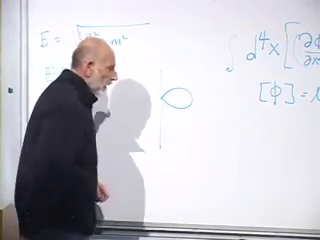
\includegraphics[width=0.72\textwidth]{lecture_03_figure_02.png}
\lectureframe{00:28:30.560}

\medskip
\begin{tikzpicture}[line width=0.8pt,scale=1.0]
  \draw[dashed] (-2.6,0) -- (0,0) -- (2.6,0);
  \fill (0,0) circle (0.055);
  \draw (0,0) .. controls (-0.85,0.7) and (-0.85,1.6) .. (0,1.6)
                .. controls (0.85,1.6) and (0.85,0.7) .. (0,0);
\end{tikzpicture}
\caption{Доска в момент перехода к скалярной самоэнергии, а затем — осторожная схематическая перерисовка топологии головастика. На снимке экрана достоверно видны петля, релятивистская и безмассовая формулы для энергии, а также часть действия; не утверждается, что заслонённые коэффициенты и обозначения различимы.}
\end{figure}

В вершине скаляр может быть поглощён и затем вновь испущен, тогда как две другие линии распространяются из точки обратно в неё саму. С точностью до численных и комбинаторных множителей поправка равна
\begin{equation}
\delta m_\phi^2\sim \lambda G_\phi(0).
\end{equation}
Пропагатор при совпадающих точках бесконечен в континуальном приближении. Эффективная теория не претендует на применимость на сколь угодно малых расстояниях, поэтому наложим \(|\Delta|\geq\delta\). Тогда
\begin{equation}
G_\phi(0)\longrightarrow G_\phi(\delta)sim\frac{1}{\delta^2},
\qquad
\delta m_\phi^2\sim\frac{\lambda}{\delta^2}sim\lambda\Lambda^2.
\end{equation}
Расходимость называется квадратичной, поскольку содержит две степени импульсного обрезания. Интегрирование в пространстве импульсов приводит к тому же выводу: чрезмерный вклад дают сколь угодно большие петлевые импульсы. Не меняет диагноза эффективной теории и то, определяется ли в конечном счёте кратчайший масштаб великим объединением, квантовой гравитацией или чем-то ещё, пока невообразимым.

Это проблема тонкой подстройки. Если \(\delta\) чрезвычайно мало, а \(\lambda\) не исключительно мало, радиационная поправка намного больше квадрата массы скаляра, наблюдаемого при низких энергиях. Голый коэффициент и петлевая поправка должны тогда взаимно компенсироваться вплоть до неправдоподобно большого числа знаков:
\begin{equation}
m_{\mathrm{physical}}^2
=m_{\mathrm{bare}}^2+\delta m_\phi^2.
\end{equation}
Массивный пропагатор не спасает положения. На расстояниях, ответственных за расходимость, \(e^{-m|\Delta|}\simeq1\). Ультрафиолетовая петля забывает о массе ещё задолго до достижения обрезания.

\section{Размерности фермионов и их пропагатор}

Теперь повторим тот же размерностный анализ для дираковского фермиона. Его свободное действие имеет вид
\begin{equation}
S_\psi=\int d^4x\,
\bar\psi\left(i\gamma^\mu\partial_\mu-m\right)\psi.
\end{equation}
Гамма-матрицы являются числовыми и безразмерными. Кинетический член содержит только одну производную, поэтому
\begin{align}
1
&=L^4[\bar\psi]L^{-1}[\psi],\\
[\psi]=[\bar\psi]&=L^{-3/2}.
\end{align}
Полуцелые степени не должны пугать; фермионы привносят половинки во многих местах.

\begin{classroomqa}
\audiencequestion{Не проще ли вывести \([\psi]\) из массового члена? \lecturetimestamp{00:36:02}}
\lecturerresponse{Да. Массовый член даёт \(L^4L^{-1}[\bar\psi\psi]=1\), следовательно, \([\bar\psi\psi]=L^{-3}\) и \([\psi]=L^{-3/2}\). Сначала был использован вывод из кинетического члена, потому что он остаётся осмысленным в безмассовой теории и показывает, почему масса фермиона входит как \(m\), а не \(m^2\).}
\end{classroomqa}

Два фермионных поля имеют размерность \(L^{-3}\), поэтому компактная размерностная запись лекции для безмассового пропагатора такова:
\begin{equation}
S(\Delta)\sim\frac{1}{|\Delta|^3}.
\end{equation}
Восстановление его матричной структуры даёт более точный числитель, требуемый лоренц-ковариантностью:
\begin{equation}
S_{ij}(\Delta)
\propto
\frac{\left(\gamma_\mu\Delta^\mu\right)_{ij}}
{\left(\Delta^2\right)^2}.
\end{equation}
Числитель добавляет одну степень длины, и потому знаменатель содержит четыре степени интервала; итоговая размерность остаётся \(L^{-3}\). Как и в скалярном случае, масса фермиона подавляет пропагатор при большом разделении, но не меняет этого короткодистанционного масштабирования.

\section{Почему замкнутая фермионная петля даёт знак минус}

Теперь можно спросить, может ли фермионная диаграмма скомпенсировать проблемный бозонный вклад в самоэнергию. Скалярная диаграмма-головастик имеет положительный знак, с точностью до положительных численных множителей, таких как степени \(\pi\) и комбинаторные коэффициенты. Замкнутая фермионная петля несёт противоположный знак.

\begin{classroomqa}
\audiencequestion{Связан ли знак минус у фермионной петли с прежним обсуждением одного полного поворота? \lecturetimestamp{00:40:21}}
\lecturerresponse{Он относится к той же фермионной знаковой структуре, но удобное доказательство здесь опирается на антисимметрию при обмене, а не на геометрическую ориентацию петли. Разрежьте две петли, обменяйте тождественные частицы и снова соедините. Обмен превращает две петли в одну и даёт знак минус только для фермионов.}
\end{classroomqa}

Этот аргумент стоит изложить полностью. Предположим, что однопетлевая диаграмма имеет знак \(\sigma\), то есть либо плюс, либо минус. Две несвязанные тождественные петли имеют знак
\begin{equation}
\sigma^2=+1.
\end{equation}
Разрежем обе петли одновременно. Теперь между разрезами распространяются две тождественные частицы. Их обычная двухчастичная волновая функция симметрична для бозонов и антисимметрична для фермионов:
\begin{align}
\Psi_B(x_1,x_2)&=+\Psi_B(x_2,x_1),\\
\Psi_F(x_1,x_2)&=-\Psi_F(x_2,x_1).
\end{align}
Антисимметрия также объясняет принцип Паули: если оба фермиона помещены в одно и то же состояние, перестановка физически ничего не меняет, но должна обратить волновую функцию в противоположную, вынуждая её обращаться в нуль.

Снова соедините разрезанные линии после обмена двух частиц. Топологически две петли превратились в одну. Амплитуда с двумя петлями без обмена была положительной. Обмен оставляет её положительной для бозонов и меняет знак для фермионов. Поэтому
\begin{equation}
\begin{aligned}
\operatorname{sign}(\text{closed boson loop})&=+1,\\
\operatorname{sign}(\text{closed fermion loop})&=-1.
\end{aligned}
\end{equation}
Этот вывод общий: каждая независимая замкнутая фермионная петля даёт множитель \(-1\).

\section{Юкавская петля}

Вернёмся к массе скаляра. Бозон не может превратиться в один фермион, потому что тогда изменилась бы чётность числа фермионов. Простейшая фермионная поправка состоит в том, что скаляр расщепляется на фермион-антифермионную пару, которые распространяются по петле и вновь рекомбинируют. Взаимодействие задаётся юкавской связью,
\begin{equation}
\mathcal L_Y=-g\phi\bar\psi\psi.
\end{equation}
Для Хиггса фермионами могут быть кварки или лептоны. Имеются две точки взаимодействия и, следовательно, два множителя \(g\).

В скалярной диаграмме-головастике была одна точка, общее положение которой можно было зафиксировать, поскольку трансляционная инвариантность лишь даёт множитель объёма пространства-времени. В юкавской петле участвуют две точки. Можно зафиксировать одну из них или, что эквивалентно, их среднее положение, но нужно проинтегрировать по их относительному смещению \(\Delta\). Каждый фермионный пропагатор вносит короткодистанционный множитель \(1/|\Delta|^3\), поэтому
\begin{equation}
\delta m_{\phi,F}^2
\sim
-g^2\int_{|\Delta|\geq\delta}d^4\Delta\,
\frac{1}{|\Delta|^6}.
\end{equation}

После того как записаны два пропагатора, интеграл по разделению и две константы связи, остаётся спросить у аудитории ещё об одном последнем множителе. Ответ — знак минус. Два пропагатора замыкаются в фермионную петлю, поэтому весь этот в остальном положительный короткодистанционный интеграл умножается на \(-1\).

Размерностный анализ уже определяет расходимость. Четыре степени длины приходят из \(d^4\Delta\), шесть стоят в знаменателе, и единственным оставшимся масштабом длины остаётся обрезание:
\begin{equation}
\int_{|\Delta|\geq\delta}
\frac{d^4\Delta}{|\Delta|^6}
\sim\frac{1}{\delta^2}.
\end{equation}
В четырёхмерных евклидовых радиальных координатах это можно записать явно:
\begin{equation}
\int_{\delta}^{R}d^4\Delta\,\frac{1}{|\Delta|^6}
=2\pi^2\int_{\delta}^{R}dr\,\frac{r^3}{r^6}
=\pi^2\left(\frac{1}{\delta^2}-\frac{1}{R^2}\right).
\end{equation}
Следы по спинорам и нормировки пропагаторов меняют коэффициент, но не квадратичную степень обрезания.\editorialnote{Радиальный интеграл — это стандартная явная версия размерностной оценки, сделанной на лекции. Он записан через евклидово расстояние, где наглядны положительность и ультрафиолетовый подсчёт степеней.}

\begin{classroomqa}
\audiencequestion{Может ли изменение порядка или выбор пределов интегрирования изменить знак? \lecturetimestamp{00:51:06}}
\lecturerresponse{Нет. Это не одномерный ориентированный интеграл, в котором пределы порождают физический знак. Это интеграл по четырём компонентам или, ещё яснее, по положительной радиальной мере. Его ультрафиолетовая величина положительна. Отрицательный вклад возникает исключительно из замкнутой фермионной петли.}
\end{classroomqa}

\begin{classroomqa}
\audiencequestion{Какова размерность юкавской константы связи \(g\)? \lecturetimestamp{00:51:51}}
\lecturerresponse{В четырёх измерениях она безразмерна. Поскольку \([\phi]=L^{-1}\) и \([\bar\psi\psi]=L^{-3}\), произведение \(\phi\bar\psi\psi\) имеет размерность \(L^{-4}\), которая в точности компенсируется \(d^4x\).}
\end{classroomqa}

Следовательно, ведущая фермионная поправка имеет вид
\begin{equation}
\delta m_{\phi,F}^2
\sim -C_F\frac{g^2}{\delta^2}
=-C_Fg^2\Lambda^2,
\end{equation}
где \(C_F>0\) содержит численные, спиновые и кратностные множители. Соответствующая скалярная петля имеет вид
\begin{equation}
\delta m_{\phi,B}^2
\sim+C_B\frac{\lambda}{\delta^2}
=+C_B\lambda\Lambda^2.
\end{equation}
Мы ещё не решили проблему тонкой подстройки, но нашли нечто необходимое: вклад с той же степенью ультрафиолетовой расходимости и противоположным знаком.

\section{Что требуется для компенсации}

Было бы чрезвычайной случайностью, если бы не связанные между собой константы связи случайно удовлетворяли
\begin{equation}
C_B\lambda=C_Fg^2
\end{equation}
именно с той точностью, которую требует большая иерархия масштабов. В лекции это сокращённо записывается как \(g^2=\lambda\), при этом опущены зависящие от соглашений и кратностные множители. Для подлинного решения нужна математическая структура, которая навязывает это соотношение, а не просто допускает его.

В этом и состоит суперсимметрический мотив. Суперсимметрия связывает бозоны и фермионы и ограничивает их константы связи такими комбинациями, при которых сокращаются многие иначе опасные расходящиеся члены. Тогда это сокращение воспроизводится от диаграммы к диаграмме, поскольку следует из симметрии, а не потому, что параметры подгоняются по одной петле за раз.

Согласование масс тоже важно. Если массы бозона и фермиона совпадают, их полные пропагаторы можно сопоставить наиболее точно. Если массы немного различаются, полные конечные результаты не сокращаются в точности, потому что пропагаторы различаются на расстояниях, сравнимых с их комптоновскими длинами волн. Тем не менее их общая асимптотика на малых расстояниях может взаимно уничтожить расходящуюся часть:
\begin{equation}
\mathcal I_B(\Delta)-\mathcal I_F(\Delta)
\quad\hbox{may be finite as}\quad \Delta\to0,
\end{equation}
где \(\mathcal I_B\) и \(\mathcal I_F\) обозначают полные бозонное и фермионное подынтегральные выражения петлевого интеграла после учета вершин, числителей и кратностей. Сами пропагаторы имеют разные размерности и непосредственно друг из друга не вычитаются. Даже когда ультрафиолетовые члены сокращаются, может остаться конечный остаток. Здесь и возникает возможность приближённой или нарушенной суперсимметрии. Точное равенство даёт наиболее чистое сокращение; достаточно контролируемое нарушение всё ещё может устранить ультрафиолетовую катастрофу, оставив наблюдаемые расщепления масс.

Таким образом, мы пришли к суперсимметрии, ещё не записав её алгебру. Цепочка рассуждений завершена:
\begin{equation}
\begin{gathered}
G_\phi(\Delta)\sim \Delta^{-2},
\qquad
\delta m_{\phi,B}^2\sim+C_B\lambda\Lambda^2,\\[0.4em]
S_\psi(\Delta)\sim \Delta^{-3},
\qquad
\delta m_{\phi,F}^2\sim-C_Fg^2\Lambda^2,\\[0.4em]
\text{symmetry-enforced matching}\\
\Longrightarrow\quad
\text{quadratic divergences cancel}.
\end{gathered}
\end{equation}
Следующая задача — понять абстрактный принцип симметрии, который обеспечивает выполнение этих соотношений, и рассмотреть конкретные примеры его действия.
\chapter{От обычной симметрии к алгебре Грассмана}

\lectureoverview{Суперсимметрия является симметрией, поэтому мы начнем с напоминания о том, что означает это слово в квантовой механике. Физическое преобразование представляется в пространстве Гильберта унитарным оператором; непрерывные преобразования порождаются бесконечно малыми, а их коммутаторы кодируют способ композиции этих преобразований. Подлинная симметрия сохраняет энергию, что эквивалентно коммутированию с гамильтонианом. Далее суперсимметрия изменяет одно предположение, общее для всех знакомых примеров: ее генераторы переводят бозоны в фермионы, а фермионы в бозоны. Построение таких генераторов естественным образом приводит к операторам рождения и уничтожения, антикоммутаторам и конечной алгебре Грассмана, в которой нечетные величины в квадрате равны нулю.}

\section{Симметрия связывает разные конфигурации}

Симметрия — не просто внешняя правильность. Это операция, которая связывает одну физическую конфигурацию с другой. Лево-правая зеркальная симметрия, например, связывает две руки. Если бы человек и окружающие законы обладали точной лево-правой симметрией, соответствующие свойства двух рук совпадали бы. В более общем случае объекты или состояния, связанные точной симметрией, должны иметь одинаковые физические величины, которые эта симметрия сохраняет. В физике частиц это часто означает равные массы; в атомной физике — равные энергии состояний, принадлежащих одному и тому же вращательному мультиплету.

Наша цель — суперсимметрия, но сначала полезно вспомнить непрерывные симметрии, такие как вращения и трансляции. Вопрос о том, является ли суперсимметрия «непрерывной» в обычном смысле, уже вызывает затруднение. Ее бесконечно малые параметры не являются обычными коммутирующими вещественными числами. Ее лучше рассматривать как градуированное расширение непрерывной симметрии, и введенная ниже арифметика Грассмана делает это утверждение достаточно точным для наших нынешних целей. \editorialnote{В современной терминологии суперсимметрия описывается как непрерывная градуированная симметрия. Это уточнение объясняет предупреждение в лекции о том, что обычное противопоставление непрерывного и дискретного плохо применимо к суперсимметрии.}

\section{Унитарные операции в пространстве Гильберта}

Квантовая система представляется вектором состояния \(\ket{\psi}\). Физическая операция симметрии представляется оператором \(U\), действующим на это состояние:
\begin{equation}
\ket{\psi}\longmapsto U\ket{\psi}.
\end{equation}
Для пространственного вращения ось и угол определяют \(U\). Если состояние содержит частицы в нескольких положениях, преобразованный кет представляет их все в повернутых положениях. Трансляция действует аналогично: она заменяет состояние другим, в котором смещена вся конфигурация.

\begin{classroomqa}
\audiencequestion{Вектор состояния принадлежит пространству Гильберта, часто бесконечномерному. Мы вращаем пространство Гильберта или обычное трехмерное пространство? \lecturetimestamp{00:04:20}}
\lecturerresponse{Оба описания относятся к одной и той же операции, но на разных уровнях. Унитарное преобразование действует на вектор в пространстве Гильберта и представляет физическое вращение конфигурации в обычном пространстве. Это не буквальное трехмерное вращение абстрактного пространства Гильберта; это представление в нем пространственного вращения.}
\end{classroomqa}

Существенное условие — унитарность:
\begin{equation}
U^\dagger U=UU^\dagger=\mathbf 1,
\qquad
U^{-1}=U^\dagger.
\end{equation}
Это сохраняет скалярные произведения и, следовательно, вероятности:
\begin{equation}
\braket{U\psi}{U\psi}
=\bra{\psi}U^\dagger U\ket{\psi}
=\braket{\psi}{\psi}.
\end{equation}

\begin{figure}[H]
\centering
\includegraphics[width=0.56\textwidth]{lecture_04_figure_02.png}
\lectureframe{00:05:56.420}
\caption{Ранний переход на доске от преобразованного состояния к условию унитарности. Кет и произведение с эрмитовым сопряжением видны, но лектор закрывает их правые части; полные уравнения приведены в выводе ниже.}
\end{figure}

Строго говоря, теорема Вигнера допускает также антиунитарные симметрии, такие как обращение времени. Преобразования, непрерывно связанные с тождественным преобразованием, которые и рассматриваются здесь, представляются унитарными операторами. \editorialnote{Возможность антиунитарности — стандартное уточнение; она не меняет обсуждения в лекции вращений, трансляций или генераторов суперсимметрии.}

\section{Бесконечно малые преобразования и генераторы}

Ничего не делать представляется как \(U=\mathbf 1\), а не \(U=0\). Достаточно малое преобразование отличается от тождественного членом, линейным по его малому параметру. Для вращения на малый угол \(\epsilon\),
\begin{equation}
U(\epsilon)=\mathbf 1+i\epsilon L+O(\epsilon^2).
\end{equation}
Унитарность в первом порядке требует
\begin{align}
U^\dagger U
&=\left(\mathbf 1-i\epsilon L^\dagger\right)
  \left(\mathbf 1+i\epsilon L\right)+O(\epsilon^2)\\
&=\mathbf 1+i\epsilon(L-L^\dagger)+O(\epsilon^2),
\end{align}
и, следовательно,
\begin{equation}
L^\dagger=L.
\end{equation}
Оператор \(L\) является генератором бесконечно малого преобразования.

Для вращений нужны три генератора, по одному для каждой независимой оси:
\begin{equation}
L_x,\qquad L_y,\qquad L_z.
\end{equation}
Вращение вокруг произвольной оси \(\widehat{\bm n}\) порождается оператором
\begin{equation}
L_{\widehat{\bm n}}=\widehat{\bm n}\cdot\bm L.
\end{equation}

\begin{classroomqa}
\audiencequestion{Можно ли сложить генераторы для осей \(x\), \(y\) и \(z\), чтобы получить вращение вокруг другой оси? \lecturetimestamp{00:07:50}}
\lecturerresponse{Да. Их линейные комбинации порождают вращения вокруг промежуточных осей. Трех независимых компонент достаточно, чтобы построить любое бесконечно малое пространственное вращение.}
\end{classroomqa}

Для вращений этими генераторами являются компоненты углового момента. Такое обозначение полезно и в более общем случае, поскольку любая непрерывная симметрия локально описывается через свои генераторы.

\section{Коммутатор как таблица умножения}

Генераторы вращений удовлетворяют
\begin{align}
[L_x,L_y]&=iL_z,&
[L_y,L_z]&=iL_x,&
[L_z,L_x]&=iL_y,
\end{align}
или, в компактной записи,
\begin{equation}
[L_i,L_j]=i\epsilon_{ijk}L_k.
\end{equation}
Символ Леви-Чивиты обращается в нуль, если два индекса совпадают, и равен \(+1\) или \(-1\) для четных или нечетных перестановок \(1,2,3\). Важный структурный факт состоит в замкнутости: коммутатор двух генераторов является еще одним генератором.

Почему именно коммутатор должен описывать геометрию вращений? Выполните малое вращение вокруг \(x\), затем вокруг \(y\), отмените вращение вокруг \(x\) и, наконец, отмените вращение вокруг \(y\). Операции не сокращаются, потому что вращения вокруг разных осей не коммутируют.

\begin{classroomqa}
\audiencequestion{Можно ли наглядно представить эту некоммутативность на примере крена, тангажа и рыскания самолета? \lecturetimestamp{00:12:36}}
\lecturerresponse{Да. Последовательные вращения вокруг осей, связанных с телом, сразу геометрически показывают, что изменение порядка меняет конечную ориентацию. Алгебра ниже является бесконечно малой версией этого хорошо известного факта.}
\end{classroomqa}

Пусть
\begin{equation}
U_x(\epsilon)=\mathbf 1+i\epsilon L_x,
\qquad
U_y(\delta)=\mathbf 1+i\delta L_y.
\end{equation}
Поскольку операторы действуют на кеты справа налево, указанная последовательность представляется как
\begin{equation}
\mathcal C
=U_y^{-1}(\delta)U_x^{-1}(\epsilon)
 U_y(\delta)U_x(\epsilon).
\end{equation}

\begin{classroomqa}
\audiencequestion{Почему операции отмены можно записывать через обратные операторы, а не через эрмитово-сопряженные? \lecturetimestamp{00:13:25}}
\lecturerresponse{Потому что преобразования унитарны: \(U^\dagger=U^{-1}\). Для бесконечно малого преобразования взятие обратного просто меняет знак у члена первого порядка, \(U_x^{-1}=\mathbf 1-i\epsilon L_x+O(\epsilon^2)\).}
\end{classroomqa}

Перемножение четырех множителей на доске превратилось в оживленное упражнение: все члены, линейные по \(\epsilon\) или \(\delta\), сокращаются, аудитория следила за смешанными членами, а временная путаница с коэффициентом 2 показала, насколько легко потерять порядок операторов. Аккуратный результат второго порядка таков:
\begin{align}
\mathcal C
&=\mathbf 1+\epsilon\delta[L_x,L_y]
  +O(\epsilon^2\delta,\epsilon\delta^2)\\
&=\mathbf 1+i\epsilon\delta L_z
  +O(\epsilon^2\delta,\epsilon\delta^2).
\end{align}
Итак, замкнутая последовательность оставляет малое вращение вокруг \(z\) на угол, пропорциональный \(\epsilon\delta\). \editorialnote{Выписанное произведение фиксирует порядок и коэффициент после исследовательского расчета в аудитории. При изменении соглашения о последовательности знак меняется на противоположный, но вывод о том, что остаточное преобразование определяется коммутатором, остается тем же.}

\begin{classroomqa}
\audiencequestion{Сделает ли изменение порядка обратных операций произведение тождественным? \lecturetimestamp{00:25:23}}
\lecturerresponse{Если каждое преобразование поставить непосредственно рядом с его собственным обратным, пары сократятся. В нетривиальной коммутаторной последовательности эти пары намеренно разделены; то, что она не схлопывается, и измеряет зависимость от порядка.}
\end{classroomqa}

Более длинные произведения действительно становятся сложнее, но никакого нового принципа в них нет.

\begin{classroomqa}
\audiencequestion{Что происходит, когда генераторов больше трех или когда имеется много малых преобразований? \lecturetimestamp{00:25:34}}
\lecturerresponse{Коммутаторов становится больше, как и технического учета, но знание замкнутой алгебры позволяет определить, как комбинируется сколь угодно большое число бесконечно малых преобразований. Конечные преобразования можно собрать из многих малых.}
\end{classroomqa}

В этом смысле алгебра коммутаторов есть таблица умножения непрерывной группы, записанная вблизи тождества.

\section{Трансляции завершают пространственный пример}

Пространственные трансляции порождаются импульсом. В принятом в лекции соглашении о знаках,
\begin{equation}
\begin{aligned}
T_x(a)&=\mathbf 1+iaP_x+O(a^2),\\
T_y(b)&=\mathbf 1+ibP_y+O(b^2),
\end{aligned}
\end{equation}
где \(a\) и \(b\) — расстояния, а не углы.

Две трансляции коммутируют. Сместите точку по \(x\), затем по \(y\), отмените трансляцию по \(x\) и отмените трансляцию по \(y\); точка вернется в исходное положение:
\begin{equation}
[P_i,P_j]=0.
\end{equation}

\begin{classroomqa}
\audiencequestion{Требуются ли силы, чтобы начать и остановить движение при переносе или вращении физического объекта? \lecturetimestamp{00:28:45}}
\lecturerresponse{Определяется не эта операция. Преобразование симметрии сопоставляет исходное состояние с математическим состоянием, в котором вся конфигурация целиком смещена или повернута. Оно не описывает динамическую траекторию, ускорение или работу, совершаемую при перемещении установки.}
\end{classroomqa}

Поворот и перенос не коммутируют. Сместите точку, поверните её вокруг начала координат, перенесите обратно вдоль исходной оси и отмените поворот; точка не вернётся туда, откуда начала. Смешанная алгебра имеет вид
\begin{equation}
[L_i,P_j]=i\epsilon_{ijk}P_k.
\end{equation}
Это соотношение означает, что сам импульс преобразуется как вектор при поворотах. Точное упражнение с индексами здесь менее важно, чем общий вывод: преобразования евклидова пространства закодированы в коммутаторах между их генераторами поворотов и переносов.

\section{Симметрия должна сохранять энергию}

Теперь перейдём от композиции преобразований к динамике. Если \(U\) действительно является симметрией системы, его применение не может изменить энергию. Пусть \(\ket{E}\) — собственное состояние энергии:
\begin{equation}
H\ket{E}=E\ket{E}.
\end{equation}
Символ \(E\) справа — это число; \(\ket{E}\) — вектор, помеченный этим собственным значением.

\begin{figure}[H]
\centering
\begin{minipage}[t]{0.43\textwidth}
\centering
\includegraphics[width=\linewidth]{lecture_04_figure_03.png}
\lectureframe{00:34:38.239}
\end{minipage}
\hfill
\begin{minipage}[t]{0.50\textwidth}
\centering
\includegraphics[width=\linewidth]{lecture_04_figure_04.png}
\lectureframe{00:36:22.376}
\end{minipage}
\caption{Преобразованный кет \(U\ket{E}\) и определяющее уравнение на собственное значение \(H\ket{E}=E\ket{E}\), выделенные на последовательных кадрах на доске.}
\end{figure}

Если \(U\) — симметрия, то \(U\ket{E}\) имеет то же собственное значение:
\begin{equation}
HU\ket{E}=EU\ket{E}.
\end{equation}
Так как \(E\) — скаляр, он коммутирует с \(U\), и можно использовать исходное уравнение на собственные значения:
\begin{align}
HU\ket{E}
&=EU\ket{E}\\
&=UE\ket{E}\\
&=UH\ket{E}.
\end{align}
Следовательно
\begin{equation}
(HU-UH)\ket{E}=0.
\end{equation}

\begin{classroomqa}
\audiencequestion{Можно ли повторить вывод, начиная с первого соотношения? \lecturetimestamp{00:35:55}}
\lecturerresponse{Начните с \(H\ket{E}=E\ket{E}\). Симметрия означает, что \(U\ket{E}\) имеет ту же энергию, так что \(HU\ket{E}=EU\ket{E}\). Перенесите скаляр \(E\) через \(U\), замените \(E\ket{E}\) на \(H\ket{E}\) и вычтите. Получается \((HU-UH)\ket{E}=0\).}
\end{classroomqa}

\begin{figure}[H]
\centering
\includegraphics[width=0.70\textwidth]{lecture_04_figure_05.png}
\lectureframe{00:38:51.066}
\caption{Полный вывод на доске. Изогнутые вспомогательные пометки связывают утверждение об одной и той же энергии с подстановкой \(E\ket{E}=H\ket{E}\); последняя строка — \((HU-UH)\ket{E}=0\).}
\end{figure}

Этот аргумент верен для каждого собственного состояния энергии. Предполагая, что эти состояния образуют полный базис, оператор, обращающий каждое из них в нуль, есть нулевой оператор:
\begin{equation}
[H,U]=0.
\end{equation}
Это критерий того, что не зависящее от времени унитарное преобразование является симметрией гамильтониана.

Для бесконечно малого преобразования,
\begin{equation}
U(\epsilon)=\mathbf 1+i\epsilon L_i+O(\epsilon^2),
\end{equation}
оператор тождества и так коммутирует с \(H\), поэтому каждый генератор должен удовлетворять
\begin{equation}
[L_i,H]=0.
\end{equation}

\begin{figure}[H]
\centering
\includegraphics[width=0.47\textwidth]{lecture_04_figure_06.png}
\lectureframe{00:42:14.296}
\caption{Критерий симметрии, сжато записанный на доске: \([U,H]=0\), а затем его форма через генератор, приведённая к стандартному виду по частично размытой нижней подписи: \([L_i,H]=0\).}
\end{figure}

Если \(L_i\) не зависит явно от времени, уравнение Гейзенберга даёт
\begin{equation}
\frac{dL_i}{dt}
=i[H,L_i]=0
\qquad(\hbar=1).
\end{equation}
Таким образом, генераторы симметрии являются сохраняющимися зарядами. Симметрия пространственных переносов даёт закон сохранения импульса; вращательная симметрия даёт закон сохранения момента импульса. \editorialnote{Оговорка об отсутствии явной зависимости от времени стандартна и неявно присутствует в лекционной формулировке закона сохранения.}

\section{Преобразуйте всю физическую систему}

Выражение «поворот является симметрией» можно употребить неправильно, если преобразуется только часть установки. Свободный спин можно повернуть, не изменяя его энергии. Однако если поместить его в фиксированное магнитное поле и повернуть только спин, его энергия Зеемана изменится. Это не опровергает вращательную симметрию; это означает, что поле удерживалось фиксированным, тогда как спин поворачивали относительно него. Если повернуть спин и поле вместе или использовать внешнее поле, которое само инвариантно, энергия не изменится.

Та же проблема возникает в атоме водорода. Смещение только электрона относительно протона изменяет расстояние между ними и, следовательно, кулоновскую энергию. Симметрия переносов действует на полную электрон-протонную систему, смещая оба на одну и ту же величину.

\begin{classroomqa}
\audiencequestion{Должно ли внешнее поле само обладать этой симметрией? \lecturetimestamp{00:43:09}}
\lecturerresponse{Либо фиксированное внешнее поле должно уже быть инвариантным относительно данной операции, либо его нужно преобразовывать вместе с остальной системой. Относительный поворот между спином и неповернутым полем — это другая физическая конфигурация, а не симметрийное преобразование всей установки.}
\end{classroomqa}

Вращательное вырождение в атоме даёт ясный положительный пример. При фиксированном угловом моменте \(l\) повороты смешивают состояния с магнитными квантовыми числами
\begin{equation}
m=-l,-l+1,\ldots,l.
\end{equation}
В отсутствие внешнего магнитного или электрического поля все члены мультиплета имеют одну и ту же энергию:
\begin{equation}
E_{l,m}=E_l.
\end{equation}
Симметрия связывает различные состояния и обусловливает их вырождение.

\section{Что меняет суперсимметрия}

Все знакомые симметрии, обсуждавшиеся до сих пор, сохраняют принадлежность к бозонам или фермионам. Поворот переводит электрон в другой электрон, а не в фотон. Цветовые повороты смешивают три цвета кварка, но не превращают кварк в глюон. Обычные внутренние и пространственно-временные симметрии могут смешивать компоненты или квантовые метки, однако их генераторы бозонны и не меняют фермионную чётность.

Суперсимметрия иная:
\begin{equation}
Q\ket{B}\sim\ket{F},
\qquad
Q\ket{F}\sim\ket{B}.
\end{equation}
Её мультиплеты пересекают границу между бозонами и фермионами. В точной суперсимметричной теории партнёры в одном мультиплете имеют одинаковую массу. Именно такое спаривание требовалось в предыдущих лекциях: согласованные бозонные и фермионные петли могут взаимно компенсировать большие ультрафиолетовые поправки к массам скаляров. Эту конструкцию трудно наглядно представить, поскольку никакое обычное пространственное движение не превращает состояние с целым спином в состояние с полуцелым спином. Поэтому далее мы будем действовать алгебраически.

\section{Прототип суперзаряда}

Пусть \(A,A^\dagger\) уничтожают и создают бозон, а \(C,C^\dagger\) уничтожают и создают фермион. Простейший эрмитов оператор, который взаимно переводит их одночастичные состояния друг в друга, имеет вид
\begin{equation}
Q=C^\dagger A+A^\dagger C.
\end{equation}
Первый член уничтожает бозон и создаёт фермион; второй уничтожает фермион и создаёт бозон. Если \(Q\) действует на однобозонное состояние, член \(A^\dagger C\) обращается в нуль, потому что нет фермиона, который можно было бы уничтожить, тогда как \(C^\dagger A\) осуществляет превращение. На однофермионном состоянии роли меняются местами.

\begin{classroomqa}
\audiencequestion{Создаёт ли эта конструкция одну частицу, являющуюся суперпозицией бозона и фермиона? \lecturetimestamp{00:52:37}}
\lecturerresponse{\(Q\) — оператор, а не состояние. Действуя на чисто бозонное состояние, он порождает фермионное состояние, а действуя на чисто фермионное состояние, он порождает бозонное состояние. Линейно действуя на уже произвольную суперпозицию, он порождает другую суперпозицию, как и любой линейный оператор.}
\end{classroomqa}

Затем в аудитории проверяют вакуум. Поскольку оба оператора уничтожения обращают его в нуль,
\begin{equation}
A\ket{0}=0,\qquad C\ket{0}=0,
\end{equation}
имеем
\begin{equation}
Q\ket{0}=0.
\end{equation}
Результат — нулевой вектор, а не вторая копия вакуума.

Этот прототип намеренно схематичен. Бозон со спином 0 может отображаться в любую из компонент фермиона со спином 1/2, поэтому самому генератору нужен спинорный индекс:
\begin{equation}
Q_\alpha\ket{B}\sim\ket{F_\alpha}.
\end{equation}
В упрощённой двухкомпонентной схеме лекции
\begin{equation}
Q_\alpha\ket{F_\beta}\sim\delta_{\alpha\beta}\ket{B}.
\end{equation}

\begin{classroomqa}
\audiencequestion{Как размеры пространств состояний могут совпадать, если бозон со спином 0 имеет одну спиновую компоненту, а фермион со спином 1/2 — две? \lecturetimestamp{00:55:02}}
\lecturerresponse{Одного неиндексированного \(Q\) недостаточно. Есть спинорные компоненты \(Q_\alpha\), каждая из которых способна породить соответствующую спиновую компоненту фермиона. Сам суперзаряд несёт половину единицы спина, потому что меняет спин на половину единицы.}
\end{classroomqa}

Операторы \(Q_\alpha\) являются фермионными, или, точнее, грассманово-нечётными. Каждый входящий в них член содержит нечётное число фермионных операторов, поэтому они меняют фермионную чётность. Обычные измеримые наблюдаемые чётны. Следует различать нечётный суперзаряд и нечётный параметр преобразования: конечное суперсимметричное преобразование строится из чётной комбинации, такой как \(\epsilon^\alpha Q_\alpha+\bar\epsilon_{\dot\alpha}\bar Q^{\dot\alpha}\), где и \(\epsilon\), и \(Q\) нечётны. \editorialnote{В лекции генераторы неформально называются числами Грассмана. Точнее, суперзаряды — это нечётные операторы, тогда как антикоммутирующие параметры — числа Грассмана; их произведение чётно и может входить в конечное преобразование.}

\section{Бозонные и фермионные алгебры операторов}

Для бозонных мод, помеченных \(i,j\),
\begin{align}
[A_i,A_j]&=0,&
[A_i^\dagger,A_j^\dagger]&=0,&
[A_i,A_j^\dagger]&=\delta_{ij}.
\end{align}
Метки могут обозначать импульс, положение, спин или любой полный одночастичный базис. Поскольку операторы рождения коммутируют,
\begin{equation}
A_i^\dagger A_j^\dagger\ket{0}
=A_j^\dagger A_i^\dagger\ket{0}.
\end{equation}
Двухбозонное состояние симметрично относительно перестановки.

Фермионные операторы удовлетворяют антикоммутационным соотношениям:
\begin{align}
\{C_i,C_j\}&=0,&
\{C_i^\dagger,C_j^\dagger\}&=0,&
\{C_i,C_j^\dagger\}&=\delta_{ij},
\end{align}
где
\begin{equation}
\{X,Y\}=XY+YX.
\end{equation}
Для одной моды
\begin{equation}
\{C^\dagger,C^\dagger\}=2(C^\dagger)^2=0,
\end{equation}
поэтому
\begin{equation}
(C^\dagger)^2=0.
\end{equation}
Сам оператор не равен нулю; его квадрат равен нулю. Он может создать один фермион в этой моде, но второе применение даёт нуль. Это принцип запрета Паули на языке операторов.

Для различных меток
\begin{equation}
C_i^\dagger C_j^\dagger\ket{0}
=-C_j^\dagger C_i^\dagger\ket{0},
\end{equation}
что выражает антисимметрию двухфермионного состояния. Алгебраическая замена
\begin{equation}
\begin{gathered}
\text{bosons: commutators}\\
\Updownarrow\\
\text{fermions: anticommutators}
\end{gathered}
\end{equation}
кодирует статистическое различие.

В одной моде может находиться много бозонов. Поэтому большое число фотонов в моде может вести себя как классическое электромагнитное поле с обычной числовой амплитудой. Фермионы не могут накапливаться в одной моде, и нечётное фермионное поле не приобретает обычного коммутирующего классического значения. Это мотивирует введение иной арифметики для учёта фермионов.

\section{Грассмановы числа и чётность}

Обычные числа коммутируют:
\begin{equation}
\alpha_i\alpha_j=\alpha_j\alpha_i.
\end{equation}
Грассмановы генераторы антикоммутируют:
\begin{equation}
\theta_i\theta_j=-\theta_j\theta_i.
\end{equation}
Если положить \(i=j\), то в числовой системе, где \(2\neq0\), получаем
\begin{equation}
\theta_i^2=0.
\end{equation}
Никакое обычное числовое значение, такое как шесть или семь, нельзя приписать \(\theta_i\). Эти символы образуют алгебру, предназначенную для учёта фермионных знаков.

Обычные коэффициенты коммутируют с грассмановыми генераторами:
\begin{equation}
\alpha\theta_i=\theta_i\alpha.
\end{equation}

\begin{classroomqa}
\audiencequestion{Какой объект получается при умножении обычного числа на грассманово число? \lecturetimestamp{01:12:32}}
\lecturerresponse{Оно остаётся нечётным грассмановым элементом. Умножение на обычный коэффициент меняет его масштаб, а не чётность. Линейная оболочка генераторов образует векторное пространство над обычными числами.}
\end{classroomqa}

Алгебра обладает \(\mathbb Z_2\)-чётностью. Обычные коэффициенты и произведения чётного числа генераторов являются чётными; генератор, как и произведение нечётного числа генераторов, нечётен:
\begin{equation}
\begin{aligned}
\text{even}\cdot\text{even}&=\text{even},\\
\text{even}\cdot\text{odd}&=\text{odd},\\
\text{odd}\cdot\text{odd}&=\text{even}.
\end{aligned}
\end{equation}

\begin{classroomqa}
\audiencequestion{Аналогично ли это правилам умножения действительных и мнимых чисел или это обобщение, подобное введению \(i\)? \lecturetimestamp{01:14:25}}
\lecturerresponse{Это обобщение арифметики, но не следует слишком далеко заходить в этой аналогии. Мнимые числа по-прежнему коммутируют и удовлетворяют \(i^2=-1\); нечётные грассмановы величины антикоммутируют и в квадрате дают нуль. Общая схема умножения по чётности не делает эти алгебры одинаковыми.}
\end{classroomqa}

Произведение, такое как \(\theta_1\theta_2\), чётно и коммутирует с каждым однородным элементом алгебры Грассмана, но не является обычным числом. Оно ненулевое, тогда как
\begin{equation}
(\theta_1\theta_2)^2=0.
\end{equation}

\begin{classroomqa}
\audiencequestion{Если \(\theta_1\theta_2\) чётно, почему это не просто обычное число? \lecturetimestamp{01:17:36}}
\lecturerresponse{Чётность означает, что элемент коммутирует в градуированной алгебре; это не означает, что он является действительным или комплексным скаляром. Его нильпотентность сразу отличает его от ненулевого обычного числа.}
\end{classroomqa}

\section{Функции грассмановых переменных}

При одном генераторе любой многочлен обрывается на члене первого порядка:
\begin{equation}
f(\theta)=\alpha+\beta\theta.
\end{equation}
Все степени \(\theta^n\) при \(n\geq2\) обращаются в нуль. Для двух генераторов наиболее общий элемент имеет вид
\begin{equation}
f(\theta_1,\theta_2)
=\alpha+\beta_1\theta_1+\beta_2\theta_2
+\gamma\theta_1\theta_2.
\end{equation}
Если записать последний моном в обратном порядке, его знак меняется:
\begin{equation}
\theta_2\theta_1=-\theta_1\theta_2.
\end{equation}

\begin{classroomqa}
\audiencequestion{Порождает ли умножение \(\theta_1\) на коэффициент \(\beta\) третью независимую грассманову переменную? \lecturetimestamp{01:18:39}}
\lecturerresponse{Нет. Оно создаёт ещё один вектор в линейной оболочке \(\theta_1\), а не новый базисный генератор. При двух независимых генераторах любой нечётный линейный член имеет вид \(\beta_1\theta_1+\beta_2\theta_2\).}
\end{classroomqa}

Для трёх генераторов упорядоченный базис таков:
\begin{equation}
1,\quad
\theta_1,\theta_2,\theta_3,\quad
\theta_1\theta_2,\theta_1\theta_3,\theta_2\theta_3,\quad
\theta_1\theta_2\theta_3.
\end{equation}
В общем случае \(n\) генераторов дают \(2^n\) упорядоченных базисных мономов. Любая аналитическая функция от конечного числа грассмановых генераторов обрывается на таком многочлене, поскольку повторяющиеся генераторы обращаются в нуль. \editorialnote{Этот \(2^n\)-мерный базис явно задаёт схему, которую лекция строит для одного, двух и трёх генераторов.}

\section{Дифференцирование по грассмановым переменным}

Для одной переменной определим
\begin{equation}
\frac{\partial}{\partial\theta}\alpha=0,
\qquad
\frac{\partial}{\partial\theta}\theta=1,
\end{equation}
так что
\begin{equation}
\frac{\partial}{\partial\theta}
(\alpha+\beta\theta)=\beta.
\end{equation}
Для двух переменных выберем левые производные и будем сохранять канонический порядок \(\theta_1\theta_2\):
\begin{align}
\frac{\partial^L f}{\partial\theta_1}
&=\beta_1+\gamma\theta_2,\\
\frac{\partial^L f}{\partial\theta_2}
&=\beta_2-\gamma\theta_1.
\end{align}
Знак минус во второй строке возникает потому, что нечётная производная должна пройти через \(\theta_1\), прежде чем продифференцировать \(\theta_2\).

Это выражается градуированным правилом произведения. Если \(A\) имеет чётность \(|A|\in\{0,1\}\), то
\begin{equation}
\frac{\partial^L}{\partial\theta}(AB)
=\left(\frac{\partial^L A}{\partial\theta}\right)B
+(-1)^{|A|}A
\left(\frac{\partial^L B}{\partial\theta}\right).
\end{equation}
По духу это обычное правило, но в нём присутствует знак, требуемый антикоммутацией. Интегрирование по грассмановым переменным также можно определить и, поскольку пространство функций конечно, оно сводится к короткой таблице. Лекция откладывает эту таблицу.

\section{Разрешение загадки с экспонентой}

С одним грассмановым генератором и обычным коэффициентом \(a\)
\begin{equation}
e^{a\theta}
=1+a\theta,
\end{equation}
поскольку все высшие степени обращаются в нуль. Для двух экспонент с одним и тем же генератором выполняется
\begin{align}
e^{a\theta}e^{b\theta}
&=(1+a\theta)(1+b\theta)\\
&=1+(a+b)\theta\\
&=e^{(a+b)\theta}.
\end{align}

Затем аудитория рассматривает различные генераторы. Непосредственное умножение даёт
\begin{equation}
e^{\theta_1}e^{\theta_2}
=(1+\theta_1)(1+\theta_2)
=1+\theta_1+\theta_2+\theta_1\theta_2.
\end{equation}
Поначалу разложение на доске наводит на мысль, что квадрат \(\theta_1+\theta_2\) может дать последний член. Один из слушателей замечает знак:
\begin{equation}
(\theta_1+\theta_2)^2
=\theta_1^2+\theta_1\theta_2
 +\theta_2\theta_1+\theta_2^2
=0.
\end{equation}

\begin{classroomqa}
\audiencequestion{Квадратичный член сокращается потому, что он содержит \(\theta_1\theta_2+\theta_2\theta_1\)? \lecturetimestamp{01:24:00}}
\lecturerresponse{Да. Эта поправка меняет вывод: \(e^{\theta_1+\theta_2}=1+\theta_1+\theta_2\), тогда как упорядоченное произведение \(e^{\theta_1}e^{\theta_2}\) тоже содержит \(\theta_1\theta_2\). Наивный закон сложения экспонент не применим к различным антикоммутирующим аргументам.}
\end{classroomqa}

Противоречия нет. Даже для обычных матриц \(e^Ae^B=e^{A+B}\) выполняется только тогда, когда \(A\) и \(B\) коммутируют. Здесь
\begin{equation}
[\theta_1,\theta_2]
=\theta_1\theta_2-\theta_2\theta_1
=2\theta_1\theta_2.
\end{equation}
Этот коммутатор чётен и коммутирует с обоими генераторами, поэтому ряд Бейкера—Кэмпбелла—Хаусдорфа обрывается:
\begin{equation}
e^{\theta_1}e^{\theta_2}
=\exp\left(
\theta_1+\theta_2+\frac12[\theta_1,\theta_2]
\right)
=e^{\theta_1+\theta_2+\theta_1\theta_2}.
\end{equation}
Поскольку аргумент экспоненты справа нильпотентен, его разложение в точности равно
\(1+\theta_1+\theta_2+\theta_1\theta_2\). \editorialnote{Этот расчёт по формуле Бейкера—Кэмпбелла—Хаусдорфа даёт то разрешение, которое лекция в аудитории оставляет в виде вопроса. Лекция правильно обнаруживает несостоятельность наивного закона, но заканчивается прежде, чем выявляется недостающий коммутаторный член.}

\begin{classroomqa}
\audiencequestion{Что это за число \(1+\theta_1\), и можно ли складывать обычную и грассманову части? \lecturetimestamp{01:26:16}}
\lecturerresponse{Это неоднородный элемент алгебры Грассмана с чётной частью \(1\) и нечётной частью \(\theta_1\). Такие суммы допустимы, но они не являются ни обычными скалярами, ни однородными нечётными элементами.}
\end{classroomqa}

Ближе к концу проверяется ещё один кажущийся парадокс:
\begin{equation}
(\theta_1+\theta_2)^2=0.
\end{equation}
Это не влечёт \(\theta_1\theta_2=0\), потому что два перекрёстных члена сокращаются, а не обращаются в нуль по отдельности.

\begin{classroomqa}
\audiencequestion{Если квадрат всякого нечётного грассманова элемента равен нулю, означает ли это, что произведение любых двух грассмановых генераторов равно нулю? \lecturetimestamp{01:32:19}}
\lecturerresponse{Нет. Равенство \((\theta_1+\theta_2)^2=0\) означает \(\theta_1\theta_2+\theta_2\theta_1=0\). Оно доказывает антикоммутацию, а не то, что какое-либо из двух упорядоченных произведений обращается в нуль. Произведение различных генераторов может быть ненулевым.}
\end{classroomqa}

\begin{classroomqa}
\audiencequestion{Предполагаем ли мы обычное определение через степенной ряд, когда записываем эти экспоненты? \lecturetimestamp{01:34:42}}
\lecturerresponse{Да, и это определение согласовано, потому что каждый ряд обрывается. Ломается не сама экспонента, а неоправданное тождество \(e^Ae^B=e^{A+B}\) для некоммутирующих \(A\) и \(B\). Поправка через коммутатор восстанавливает правильный закон композиции.}
\end{classroomqa}

Такой исследовательский финал уместен. Обычные симметрии привели нас от унитарных преобразований к генераторам и коммутаторам; суперсимметрия привела нас от нечётных генераторов к антикоммутирующим переменным. В обоих случаях центральным объектом является закон умножения. Для вращений он проявляется в \([L_i,L_j]\); для грассмановых экспонент — в коммутаторном члене, который препятствует наивному сложению. Эта алгебра непривычна, но она непротиворечива, конечна и в точности подходит для фермионных преобразований, которых требует суперсимметрия.
\chapter{Суперзаряды, замыкание и суперпространство}

\lectureoverview{Суперсимметрия трудна не потому, что её правила многочисленны, а потому, что они соединяют идеи, которые обычная физика держит раздельно. Мы начнём с переменных Грассмана, нечётные элементы которых антикоммутируют, а функции от них обрываются после конечного числа членов. Их алгебра производных затем даёт модель для нечётных генераторов симметрии. Бозонный и фермионный осцилляторы дают простейшие суперзаряды: их антикоммутатор есть гамильтониан, так что обмен бозонов и фермионов неотделим от трансляции по времени. Ту же алгебру можно геометрически представить как трансляции по грассмановым направлениям расширенного пространства-времени, называемого суперпространством.}

\section{Почему, прежде чем двигаться дальше, нужно сделать шаг назад}

Суперсимметрия относится к числу самых абстрактных конструкций в физике. Она похожа на вращения и трансляции, поскольку является симметрией, но не помещается в обычное пространство-время, если не расширить само понятие координаты. Её естественные параметры — грассмановы величины: объекты, которые можно складывать и умножать, но которые антикоммутируют, а не коммутируют.

Вот почему прямой переход к окончательной алгебре был бы бесполезен. Сначала мы приведём нечётную арифметику в рабочий вид, затем напомним, как организованы обычные непрерывные симметрии, и лишь потом соединим эти две идеи. Путь длиннее, но каждый шаг подготавливает следующий.

\section{Алгебра Грассмана в рабочем виде}

\subsection{Нечётные и чётные элементы}

Пусть \(\epsilon_i\) обозначают независимые образующие Грассмана. Они удовлетворяют
\begin{equation}
\epsilon_i\epsilon_j=-\epsilon_j\epsilon_i,
\qquad
\{\epsilon_i,\epsilon_j\}=0.
\end{equation}
Полагая \(i=j\), получаем
\begin{equation}
2\epsilon_i^2=0,
\qquad
\epsilon_i^2=0,
\end{equation}
над вещественными или комплексными числами. Каждая образующая не равна нулю; нулю равен только её квадрат.

Каждый однородный элемент имеет чётность. Произведение, содержащее нечётное число образующих Грассмана, нечётно, а произведение, содержащее чётное число, чётно:
\begin{align}
\text{odd}\times\text{odd}&=\text{even},\\
\text{odd}\times\text{even}&=\text{odd},\\
\text{even}\times\text{even}&=\text{even}.
\end{align}
Чётные элементы коммутируют с однородными элементами. Два нечётных элемента антикоммутируют. Поэтому
\begin{equation}
n\epsilon_i=\epsilon_i n,
\qquad
\epsilon_i\epsilon_j=-\epsilon_j\epsilon_i,
\end{equation}
когда \(n\) чётен.

Чётный элемент не обязан быть обычным вещественным или комплексным числом. Произведение \(\epsilon_1\epsilon_2\), например, чётно и нильпотентно. Обычные числа образуют скалярную часть алгебры, а чётные произведения дают дополнительные коммутирующие элементы.

\begin{classroomqa}
\audiencequestion{Есть ли различие между алгеброй Грассмана и числами Грассмана, или это одно и то же? \lecturetimestamp{00:06:45}}
\lecturerresponse{Элементы — это числа Грассмана; алгебра — совокупность этих элементов вместе с правилами их сложения и умножения. Поэтому в нестрогой речи можно иметь в виду один и тот же объект, но полезно различать сами объекты, с которыми работают, и правила, по которым с ними работают.}
\end{classroomqa}

\subsection{Разложения функций конечны}

Функция одной переменной Грассмана имеет только две возможные степени:
\begin{equation}
f(\epsilon)=a+b\epsilon.
\end{equation}
Члена \(\epsilon^2\) нет. Для двух независимых образующих
\begin{equation}
f(\epsilon_1,\epsilon_2)
=a+b_1\epsilon_1+b_2\epsilon_2+c\epsilon_1\epsilon_2.
\end{equation}
Разложение обрывается после того, как появились обе образующие. Для \(n\) независимых образующих упорядоченные мономы образуют базис размерности \(2^n\):
\begin{equation}
1,\quad
\epsilon_i,\quad
\epsilon_i\epsilon_j,\quad
\ldots,\quad
\epsilon_1\epsilon_2\cdots\epsilon_n.
\end{equation}
\editorialnote{Конечномерное утверждение размерности \(2^n\) — это общий образец, лежащий в основе примеров с одной и двумя образующими. Можно определить и бесконечную алгебру Грассмана, но каждый используемый здесь многочлен содержит лишь конечное число образующих.}

Когда две вещественные образующие объединяют в комплексную пару \(\theta,\bar\theta\), общую функцию при выбранном порядке можно записать как
\begin{equation}
f(\theta,\bar\theta)
=a+\bar b\,\theta+\bar\theta\,b+c\,\bar\theta\theta.
\end{equation}
Черта указывает на используемое здесь обозначение комплексной пары. Если поменять порядок в последнем произведении, знак изменится:
\begin{equation}
\bar\theta\theta=-\theta\bar\theta.
\end{equation}

Обычно всей функции удобно приписать определённую чётность. Если \(f\) чётна, то \(a\) и \(c\) чётны, а \(b\) и \(\bar b\) нечётны. Если \(f\) нечётна, эти назначения обращаются. Сами коэффициенты могут принадлежать большей алгебре Грассмана, при условии что они не зависят от тех конкретных переменных, по которым выполняется разложение.

\begin{classroomqa}
\audiencequestion{Можно ли подставить переменную Грассмана в тригонометрические или другие аналитические функции? \lecturetimestamp{00:11:06}}
\lecturerresponse{Да, но степенной ряд обрывается сразу. Для одной нечётной образующей
\[
\sin\epsilon=\epsilon,\qquad
\cos\epsilon=1,\qquad
e^\epsilon=1+\epsilon.
\]
Привычные названия сохраняются, но степеней слишком мало, чтобы функции приобрели свою обычную аналитическую сложность.}
\end{classroomqa}

\section{Дифференцирование — это учёт знаков}

Мы используем левую производную Грассмана. Её определяющие локальные правила таковы
\begin{equation}
\partial_\theta a=0,
\qquad
\partial_\theta(\theta B)=B,
\end{equation}
если \(a\) и \(B\) не зависят от \(\theta\). Перед дифференцированием перенесите соответствующую \(\theta\) влево. Каждый проход через другой нечётный множитель меняет знак.

Например, если \(b\) нечётен,
\begin{equation}
b\theta=-\theta b,
\qquad
\partial_\theta(b\theta)=-b.
\end{equation}
С самой производной не произошло ничего загадочного. Минус возник ещё до дифференцирования, когда нечётные множители были переставлены.

\subsection{Вычисление для двух переменных}

Вернёмся к
\begin{equation}
f(\theta,\bar\theta)
=a+\bar b\,\theta+\bar\theta\,b+c\,\bar\theta\theta.
\end{equation}
Предположим сначала, что \(f\) чётна. Тогда \(\bar b\) нечётен, а \(c\) чётен. Переставляя члены, содержащие \(\theta\),
\begin{align}
\bar b\,\theta&=-\theta\bar b,\\
c\,\bar\theta\theta&=-\theta c\,\bar\theta.
\end{align}
Следовательно,
\begin{equation}
\partial_\theta f=-\bar b-c\bar\theta.
\end{equation}

Если \(f\) нечётна, то \(\bar b\) чётен, а \(c\) нечётен. В первом члене перестановка не проходит ни через один нечётный коэффициент, тогда как в последнем \(\theta\) проходит через два нечётных множителя, \(c\) и \(\bar\theta\). Два знака минус сокращаются:
\begin{equation}
\partial_\theta f=\bar b+c\bar\theta.
\end{equation}

\begin{classroomqa}
\audiencequestion{Почему в примере с чётной функцией оба оставшихся члена несут минусы? \lecturetimestamp{00:16:49}}
\lecturerresponse{Первый знак возникает при переносе \(\theta\) мимо нечётного коэффициента \(\bar b\). В последнем члене \(c\) чётен, но \(\theta\) должна пройти мимо нечётной переменной \(\bar\theta\). В каждой перестановке происходит проход через один нечётный множитель, поэтому каждая даёт один знак минус.}
\end{classroomqa}

Ответ зависит от соглашения о порядке, но сама математика — нет. Если бы мы начали с \(c\theta\bar\theta\), а не с \(c\bar\theta\theta\), выписанный коэффициент отличался бы знаком, и формула для производной соответственно изменилась бы.

\begin{classroomqa}
\audiencequestion{Можно ли было записать последний член, поменяв местами \(\theta\) и \(\bar\theta\), и имеет ли возникающий знак более глубокий смысл? \lecturetimestamp{00:18:50}}
\lecturerresponse{Его можно записать в любом порядке, но при перестановке двух нечётных переменных знак меняется. Этот знак можно поглотить в коэффициент \(c\). На данном этапе эффект сводится к учёту: порядок важен, чётность не меняется, и смена знака никогда не превращает нечётный объект в чётный. Физический смысл появляется тогда, когда тот же самый учёт обеспечивает фермионную статистику и суперсимметрию.}
\end{classroomqa}

\begin{classroomqa}
\audiencequestion{Разве коэффициенты \(a,b,c\) просто берутся из поля комплексных чисел? \lecturetimestamp{00:20:47}}
\lecturerresponse{Они могут быть обычными комплексными числами, когда по чётности от них требуется быть чётными, но могут и содержать образующие, отличные от выбранных \(\theta,\bar\theta\). Интересующая нас алгебра обычно содержит все комплексные скаляры вместе с выбранным набором нечётных образующих и их произведениями.}
\end{classroomqa}

\begin{classroomqa}
\audiencequestion{Производные от чётной и нечётной функций выглядят противоположными. Является ли это общей симметрией? \lecturetimestamp{00:22:31}}
\lecturerresponse{Нет, само по себе нет. Знаки механически определяются чётностью каждого коэффициента и числом нечётных множителей, через которые приходится пройти. Иногда два ответа случайно оказываются противоположными, но надёжное правило проще: каждая перестановка двух нечётных объектов вносит один знак минус.}
\end{classroomqa}

\subsection{Координата и производная как операторы}

Есть поучительный обычный аналог. Пусть умножение на \(x\) и дифференцирование по \(x\) действуют на произвольную функцию \(g(x)\). Тогда
\begin{align}
\partial_x\!\left(xg\right)&=g+xg',\\
x\partial_xg&=xg',
\end{align}
поэтому
\begin{equation}
[\partial_x,x]g=g.
\end{equation}
Поскольку это верно для всякой \(g\),
\begin{equation}
[\partial_x,x]=1.
\end{equation}
При \(p=-i\partial_x\) это привычная алгебра координаты и импульса в единицах, где \(\hbar=1\).

В аналоге для Грассмана используется антикоммутатор. Возьмём
\begin{equation}
f(\theta)=a+\theta b,
\end{equation}
где \(a\) чётен, а \(b\) нечётен, так что \(f\) чётна. Сначала
\begin{equation}
\theta\partial_\theta f=\theta b.
\end{equation}
В противоположном порядке
\begin{align}
\partial_\theta(\theta f)
&=\partial_\theta(\theta a+\theta^2b)\\
&=a.
\end{align}
Складывая оба порядка, получаем исходную функцию:
\begin{equation}
\left(\partial_\theta\theta+\theta\partial_\theta\right)f
=a+\theta b=f.
\end{equation}
Следовательно,
\begin{equation}
\boxed{\{\partial_\theta,\theta\}=1.}
\end{equation}
Производная \(\partial_\theta\) сама нечётна. Поэтому её каноническое соотношение с нечётной координатой имеет вид антикоммутатора.

\begin{classroomqa}
\audiencequestion{Можно ли использовать функцию, содержащую и чётную, и нечётную части, вместо того чтобы приписывать ей определённую чётность? \lecturetimestamp{00:31:05}}
\lecturerresponse{Такие неоднородные элементы можно строить, но вычисления обычно организуют в виде однородных чётных и нечётных объектов. Определённая чётность делает каждый знак в градуированном произведении однозначным; со смешанным объектом работают, разлагая его на чётную и нечётную части.}
\end{classroomqa}

\begin{classroomqa}
\audiencequestion{Должна ли была пробная функция \(g(x)\) в вычислении обычного коммутатора быть нечётной? \lecturetimestamp{00:31:45}}
\lecturerresponse{Нет. Это была обычная функция обычной коммутирующей координаты. Её ввели только для того, чтобы показать, как доказывается операторное тождество \([\partial_x,x]=1\), прежде чем повторить тот же довод для пары Грассмана \(\partial_\theta,\theta\).}
\end{classroomqa}

\begin{classroomqa}
\audiencequestion{Существует ли предел числу независимых грассмановых генераторов? \lecturetimestamp{00:32:16}}
\lecturerresponse{Алгебраического верхнего предела нет. При \(n\) генераторах базис содержит \(2^n\) мономов, так что учёт быстро усложняется, но сама конструкция работает для любого конечного \(n\).}
\end{classroomqa}

\subsection{Интегрирование}

Интеграл по одной грассмановой переменной фиксируется условиями
\begin{equation}
\int d\theta\,1=0,
\qquad
\int d\theta\,\theta=1.
\end{equation}
Следовательно, для \(f(\theta)=a+\theta b\),
\begin{equation}
\int d\theta\,f(\theta)=b=\partial_\theta f(\theta).
\end{equation}
Тем самым интегрирование и дифференцирование извлекают одну и ту же компоненту. Это интеграл Березина. Его нормировка — единственный простой выбор, совместимый с инвариантностью относительно сдвигов и интегрированием по частям для грассмановых переменных. \editorialnote{Правила для компонент точно формулируют высказанное на лекции утверждение о том, что интегрирование и дифференцирование по грассмановым переменным — одна и та же операция.}

\section{Обычная симметрия как отправная точка}

Рассмотрим непрерывную унитарную группу с эрмитовыми генераторами \(G_i\). В окрестности единицы,
\begin{equation}
U(\alpha)=\mathbf 1+i\alpha^iG_i+O(\alpha^2),
\end{equation}
где \(\alpha^i\) — обычные коммутирующие параметры. Закон умножения в бесконечно малом задаётся алгеброй Ли
\begin{equation}
[G_i,G_j]=i f_{ij}{}^{k}G_k.
\end{equation}
Константы \(f_{ij}{}^k\) — это структурные константы. Замкнутость означает, что коммутатор любых двух генераторов даёт линейную комбинацию генераторов, уже принадлежащих алгебре.

Для вращений,
\begin{equation}
[L_i,L_j]=i\varepsilon_{ijk}L_k.
\end{equation}
Три эрмитовы компоненты можно объединить в неэрмитовы лестничные операторы
\begin{equation}
L_\pm=L_x\pm iL_y,
\end{equation}
которые повышают или понижают магнитное квантовое число \(m\) на единицу. Комплексные комбинации полезны и при этом не меняют эрмитовости лежащих в основе физических генераторов.

В общем базисе антисимметричными обязаны быть только первые два индекса \(f_{ij}{}^k\). Для компактной алгебры с инвариантной ортонормированной метрикой можно опустить последний индекс и выбрать соглашения, при которых \(f_{ijk}\) полностью антисимметричен, как это и бывает для вращений. \editorialnote{Эта оговорка отделяет всегда имеющую место антисимметрию коммутатора от более сильного свойства, доступного в привычном базисе вращений.}

Чтобы \(G_i\) порождал действительную симметрию не зависящей от времени системы,
\begin{equation}
[H,G_i]=0.
\end{equation}
Эквивалентно, \(G_i\) отображает каждое собственное подпространство энергии в себя. При отсутствии явной зависимости от времени уравнение Гейзенберга даёт
\begin{equation}
\frac{dG_i}{dt}=i[H,G_i]=0,
\end{equation}
так что генератор является сохраняющимся зарядом.

Обычные наблюдаемые величины чётны. Фермионное поле нечётно, но отдельное нечётное поле само по себе не является измеримой наблюдаемой величиной; физические операторы содержат чётное суммарное число фермионных множителей. Суперсимметрия меняет чётность генераторов, а не ту чётность, которой должны обладать наблюдаемые результаты.

Удобное обозначение для всех случаев — градуированный коммутатор
\begin{equation}
[X,Y]_{\mathrm{gr}}
=XY-(-1)^{|X||Y|}YX.
\end{equation}
Это обычный коммутатор, если хотя бы один из операторов чётный, и антикоммутатор, если оба нечётные.

\section{Наименьший суперсимметричный осциллятор}

\subsection{Одна бозонная мода и одна фермионная мода}

Возьмём одну бозонную моду с операторами рождения и уничтожения \(a_+\) и \(a_-\):
\begin{equation}
[a_-,a_+]=1,
\qquad
[a_+,a_+]=[a_-,a_-]=0.
\end{equation}
Её оператор числа равен
\begin{equation}
N_B=a_+a_-,
\end{equation}
а число заполнения может принимать значения \(0,1,2,\ldots\).

Для одной фермионной моды введём \(c_+\) и \(c_-\):
\begin{equation}
\{c_-,c_+\}=1,
\qquad
\{c_+,c_+\}=\{c_-,c_-\}=0.
\end{equation}
Поэтому
\begin{equation}
c_+^2=c_-^2=0,
\qquad
N_F=c_+c_-,
\end{equation}
и число заполнения может быть только \(0\) или \(1\). Бозонные операторы чётны, фермионные операторы нечётны, и каждый \(a_\pm\) коммутирует с каждым \(c_\pm\).

\editorialnote{Нильпотентность ограничивает фермионную моду одним заполненным состоянием. У бозонной моды заполнение не ограничено; краткая противоположная формулировка в аудиторном обсуждении снимается самой алгеброй осциллятора.}

Предположим, что бозон и фермион имеют одинаковую энергию покоя \(m\), и определим
\begin{equation}
Q=\sqrt m\,a_+c_-,
\qquad
\bar Q=Q^\dagger=\sqrt m\,a_-c_+.
\end{equation}
Оператор \(Q\) уничтожает один фермион и создаёт один бозон. Его сопряжённый уничтожает один бозон и создаёт один фермион. Каждый из них содержит один фермионный оператор и потому нечётен.

На числовых состояниях их действие записывается явно:
\begin{align}
Q\ket{n,1}
&=\sqrt{m(n+1)}\,\ket{n+1,0},
&
Q\ket{n,0}&=0,\\
\bar Q\ket{n,0}
&=\sqrt{mn}\,\ket{n-1,1},
&
\bar Q\ket{n,1}&=0.
\end{align}
\editorialnote{Формулы для числовых состояний представляют собой непосредственно нормированную форму описанного в лекции действия по замене частицы.}

\subsection{Антикоммутатор замыкается на энергии}

Градуированный аналог поиска алгебры Ли состоит в вычислении
\begin{align}
\{Q,\bar Q\}
&=Q\bar Q+\bar Q Q\\
&=m\left(a_+c_-a_-c_+
        +a_-c_+a_+c_-\right).
\end{align}
Поскольку \(a\) чётны, они проходят через \(c\) без знака:
\begin{equation}
\{Q,\bar Q\}
=m\left(a_+a_-c_-c_+
        +a_-a_+c_+c_-\right).
\end{equation}
Теперь воспользуемся
\begin{equation}
c_-c_+=1-c_+c_-,
\qquad
a_-a_+=a_+a_-+1.
\end{equation}
Тогда
\begin{align}
\{Q,\bar Q\}
&=m\left[
N_B(1-N_F)+(N_B+1)N_F
\right]\\
&=m(N_B+N_F).
\end{align}
Временный лишний множитель 2, возникший при перестановке в ходе вывода у доски, исчезает: один вклад даёт \(N_B\), другой — \(N_F\).

Для покоящихся частиц с одинаковыми массами гамильтониан имеет вид
\begin{equation}
H=m(N_B+N_F).
\end{equation}
Следовательно,
\begin{equation}
\boxed{\{Q,\bar Q\}=H.}
\end{equation}

\begin{figure}[H]
\centering
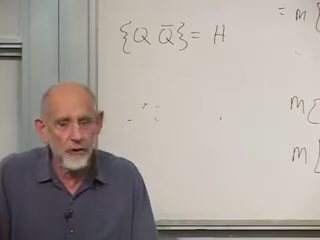
\includegraphics[width=0.62\textwidth]{lecture_05_figure_02.png}
\lectureframe{00:55:46.300}
\caption{Выделенное на доске центральное соотношение замыкания. Фигурные скобки и \(Q,\bar Q,H\) видны; запятая восстанавливается по стандартному обозначению антикоммутатора.}
\end{figure}

Аддитивный нуль энергии выбран так, что пустое состояние имеет \(H=0\). Для суперсимметричного осциллятора это естественное соглашение: бозонный и фермионный вклады нулевых колебаний взаимно сокращаются. \editorialnote{В лекции сразу используется полная энергия покоя и отдельно не выписываются члены нулевой энергии; указанное соглашение делает этот выбор явным.}

Гамильтониан чётен. Он также является генератором симметрии: он порождает сдвиги по времени. Поэтому нечётные генераторы не замыкаются между собой, если не включить чётный генератор временных сдвигов.

\begin{classroomqa}
\audiencequestion{Какой член этого соотношения чётный? Это гамильтониан? \lecturetimestamp{00:58:24}}
\lecturerresponse{Да. Энергия — обычная наблюдаемая величина, поэтому \(H\) чётен. Суперзаряд \(Q\) нечётен, а произведение двух нечётных величин чётно; соответственно, \(\{Q,\bar Q\}\) может равняться \(H\). Нечётный и чётный генераторы связаны коммутатором, а не антикоммутатором.}
\end{classroomqa}

\subsection{Завершение алгебры}

Соотношения для генераторов одинаковой чётности сразу очевидны:
\begin{equation}
\{Q,Q\}=2Q^2=0,
\qquad
\{\bar Q,\bar Q\}=2\bar Q^2=0,
\end{equation}
поскольку \(Q^2\) содержит \(c_-^2\), а \(\bar Q^2\) содержит \(c_+^2\).

Остаётся соотношение с \(H\). Пусть
\begin{equation}
H\ket{E}=E\ket{E}.
\end{equation}
Если массы бозона и фермиона равны, \(Q\) заменяет одну частицу другой, не изменяя энергии. Следовательно, \(Q\ket{E}\) либо равно нулю, либо является другим собственным состоянием с тем же собственным значением:
\begin{equation}
H Q\ket{E}=E Q\ket{E}.
\end{equation}
С другой стороны,
\begin{equation}
QH\ket{E}=Q(E\ket{E})=E Q\ket{E}.
\end{equation}
Вычитая,
\begin{equation}
[H,Q]\ket{E}=0.
\end{equation}
Если собственные состояния энергии образуют полный базис, то это верно как операторное тождество:
\begin{equation}
[H,Q]=0,
\qquad
[H,\bar Q]=0.
\end{equation}

\begin{classroomqa}
\audiencequestion{Что происходит, если массы бозона и фермиона не совпадают? \lecturetimestamp{01:01:16}}
\lecturerresponse{Тогда замена одного другим меняет энергию, так что предлагаемый суперзаряд не коммутирует с гамильтонианом, и простая суперсимметрия теряется. Для
\[
H=m_BN_B+m_FN_F,
\]
явный результат имеет вид
\[
[H,Q]=(m_B-m_F)Q.
\]
Он обращается в нуль в точности при \(m_B=m_F\). \editorialnote{Коммутатор при неравных массах есть прямая операторная форма аргумента об изменении энергии и делает условие равенства масс явным.}}
\end{classroomqa}

\begin{classroomqa}
\audiencequestion{Нельзя ли повторить аргумент с собственными состояниями энергии чуть медленнее? \lecturetimestamp{01:01:37}}
\lecturerresponse{Начнём с \(H\ket{E}=E\ket{E}\). Равенство масс влечёт, что \(Q\ket{E}\) имеет ту же определённую энергию \(E\), так что \(HQ\ket{E}=EQ\ket{E}\). В другом порядке получается \(QH\ket{E}=QE\ket{E}=EQ\ket{E}\), потому что \(E\) — обычный скаляр. Их разность обращается в нуль на каждом собственном состоянии энергии. Полнота затем переносит это утверждение с этих состояний на операторное уравнение \([H,Q]=0\).}
\end{classroomqa}

Итак, полная игрушечная алгебра имеет вид
\begin{align}
\{Q,\bar Q\}&=H,\\
\{Q,Q\}&=\{\bar Q,\bar Q\}=0,\\
[H,Q]&=[H,\bar Q]=0.
\end{align}
Суперзаряды являются сохраняющимися нечётными зарядами. Ещё более удивительно то, что их алгебра смешивает операцию, меняющую тип частицы, с генератором пространственно-временного сдвига.

\section{Почему гамильтониан является генератором сдвигов по времени}

В этой предельно упрощённой модели нет пространственной координаты, но есть время. Уравнение Шрёдингера имеет вид
\begin{equation}
i\frac{\partial}{\partial t}\ket{\psi(t)}
=H\ket{\psi(t)}.
\end{equation}

\begin{figure}[H]
\centering
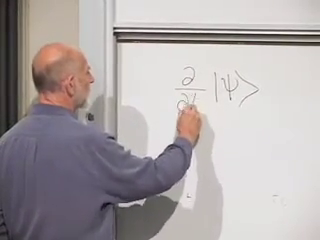
\includegraphics[width=0.56\textwidth]{lecture_05_figure_03.png}
\lectureframe{01:07:26.300}
\caption{Производная по времени записана рядом с \(\ket{\psi}\). Рука закрывает часть знаменателя; полное уравнение Шрёдингера приведено выше.}
\end{figure}

Для конечного сдвига \(\delta\),
\begin{equation}
\ket{\psi(t+\delta)}
=e^{-iH\delta}\ket{\psi(t)}.
\end{equation}
Разлагая по первому порядку,
\begin{equation}
\ket{\psi(t+\delta)}
=\left(\mathbf 1-i\delta H\right)\ket{\psi(t)}
+O(\delta^2).
\end{equation}
Таким образом, \(H\) — бесконечно малый генератор, сдвигающий состояние по времени.

Внутренние симметрии, такие как изоспин и цвет, тоже меняют метки частиц. Изоспин может смешивать состояния протона и нейтрона; цветовые вращения смешивают красные, зелёные и синие кварки. Однако никакая композиция этих внутренних преобразований не сдвигает систему в пространстве или во времени. С суперсимметрией дело обстоит иначе:
\begin{equation}
\begin{gathered}
\text{odd particle-changing transformation}\\
\mathrel{\stackrel{\{\ ,\ \}}{\Longrightarrow}}\\
\text{time translation}
\end{gathered}
\end{equation}
Это и есть указание на то, что нечётные генераторы сами могут быть сдвигами, но вдоль координат, отличных от обычных.

\section{Суперпространство}

\subsection{Функция времени и нечётных координат}

Введём функцию
\begin{equation}
\Psi=\Psi(\theta,\bar\theta,t).
\end{equation}
Её можно рассматривать как волновую функцию в игрушечной модели или, более общо, как суперполе. Поскольку разложение по нечётным координатам обрывается,
\begin{equation}
\Psi(\theta,\bar\theta,t)
=A(t)+\bar\chi(t)\theta
+\bar\theta\chi(t)+F(t)\bar\theta\theta.
\end{equation}
Этот единый объект объединяет в себе чётные и нечётные компонентные функции. \editorialnote{В этом компонентном разложении используется полином Грассмана, введённый ранее; это стандартное явное содержание функции на игрушечном суперпространстве.}

Обычный сдвиг по времени оставляет \(\theta,\bar\theta\) неизменными и переводит
\begin{equation}
t\longmapsto t+\delta.
\end{equation}
В первом порядке,
\begin{equation}
\Psi(\theta,\bar\theta,t+\delta)
=\Psi(\theta,\bar\theta,t)
+\delta\,\partial_t\Psi(\theta,\bar\theta,t).
\end{equation}

\begin{figure}[H]
\centering
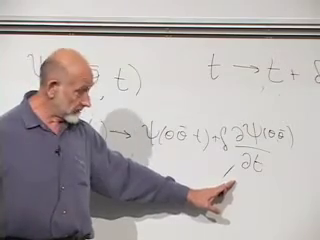
\includegraphics[width=0.72\textwidth]{lecture_05_figure_04.png}
\lectureframe{01:13:15.060}
\caption{На доске \(t\to t+\delta\) помещено над изменением \(\Psi\) в первом порядке, причём член с производной указан непосредственно.}
\end{figure}

\subsection{Сдвиг в нечётном направлении}

Теперь введём преобразование, сдвигающее нечётную координату:
\begin{equation}
\theta\longmapsto\theta+\epsilon,
\end{equation}
где \(\epsilon\) — ещё один нечётный параметр Грассмана. Одновременно пусть время получает чётное нильпотентное смещение,
\begin{equation}
t\longmapsto t+i\bar\theta\epsilon.
\end{equation}
И \(\bar\theta\), и \(\epsilon\) нечётны, так что их произведение чётно и его можно согласованно прибавить к чётной координате \(t\).

Перенеся параметр влево,
\begin{equation}
i\bar\theta\epsilon=-i\epsilon\bar\theta.
\end{equation}
Поэтому индуцированная вариация имеет вид
\begin{align}
\delta_\epsilon\Psi
&=\epsilon\,\partial_\theta\Psi
-i\epsilon\bar\theta\,\partial_t\Psi\\
&=\epsilon q_0\Psi,
\end{align}
где
\begin{equation}
q_0=\partial_\theta-i\bar\theta\partial_t.
\end{equation}
Этот нечётный дифференциальный оператор является генератором комбинированного сдвига. Совместимый сопряжённый генератор, использующий левые производные, имеет вид
\begin{equation}
\bar q_0=-\partial_{\bar\theta}
+i\theta\partial_t.
\end{equation}

Точные знаки зависят от того, используются ли левые или правые производные по Грассману и от того, как сопряжение обращает порядок нечётных множителей. То, что не должно зависеть от соглашения, — это замыкание на трансляцию по времени. При приведённых выше определениях,
\begin{align}
\{q_0,\bar q_0\}
&=i\{\partial_\theta,\theta\}\partial_t
+i\{\bar\theta,\partial_{\bar\theta}\}\partial_t\\
&=2i\partial_t.
\end{align}
Член с производными по двум переменным обращается в нуль, как и член, квадратичный по нечётным координатам. Два смешанных члена дают по \(i\partial_t\) каждый.

Поскольку для состояний в представлении Шрёдингера \(H=i\partial_t\),
\begin{equation}
\{q_0,\bar q_0\}=2H.
\end{equation}
Если ввести нормировку
\begin{equation}
q=\frac{q_0}{\sqrt2},
\qquad
\bar q=\frac{\bar q_0}{\sqrt2},
\end{equation}
то
\begin{equation}
\boxed{\{q,\bar q\}=H.}
\end{equation}
\editorialnote{В лекции намеренно проделывается вычисление с неуверенными знаками, а затем обнаруживается множитель два. Показанное соглашение с левыми производными сохраняет этот аудиторный расчёт, одновременно фиксируя одну самосогласованную нормировку. Другие стандартные соглашения перераспределяют знаки между сдвигами координат и генераторами.}

\begin{classroomqa}
\audiencequestion{Откуда берётся последний множитель два в антикоммутаторе суперпространства? \lecturetimestamp{01:24:21}}
\lecturerresponse{Есть два равных смешанных вклада. Один возникает из \(\{\partial_\theta,\theta\}=1\), а другой — из \(\{\partial_{\bar\theta},\bar\theta\}=1\). Каждый умножает производную по времени. Поэтому ненормированные генераторы дают \(2i\partial_t\); множитель \(1/\sqrt2\) в каждом суперзаряде восстанавливает прежнюю нормировку.}
\end{classroomqa}

\begin{classroomqa}
\audiencequestion{Использовалось ли в построении предположение, что \(\epsilon\) мало? \lecturetimestamp{01:24:51}}
\lecturerresponse{Использовалась нильпотентность, а не обычная численная малость. Поскольку \(\epsilon^2=0\), любое разложение по одной \(\epsilon\) обрывается после первого порядка. Называть этот параметр бесконечно малым или малым — полезная аналогия, но обрыв разложения точен.}
\end{classroomqa}

\editorialnote{Параметры Грассмана не имеют обычной положительной величины. Их роль бесконечно малых параметров обусловлена нильпотентностью и точным обрывом разложения.}

\subsection{Геометрический смысл}

Теперь эта алгебра имеет две эквивалентные реализации. В осцилляторной картине \(Q\) и \(\bar Q\) заменяют фермионы бозонами, а бозоны — фермионами. В геометрической картине \(q\) и \(\bar q\) сдвигают функцию по нечётным направлениям, вызывая при этом обычный сдвиг по времени. В обеих картинах,
\begin{equation}
\begin{gathered}
\{\text{supercharge},\text{conjugate supercharge}\}\\
=\text{time-translation generator}.
\end{gathered}
\end{equation}

Обобщённое координатное пространство, содержащее \(t,\theta,\bar\theta\), называется суперпространством. В релятивистской теории поля оно также содержит обычные пространственные координаты, и суперзаряды замыкаются на полный импульс пространства-времени \(P_\mu\), а не только на \(H=P_0\). Искривление этой структуры ведёт к супергравитации.

В одном смысле переменные Грассмана — это эффективное средство учёта бозонов и фермионов. В другом отношении соотношение замыкания говорит о гораздо более глубоком: различие между типом частицы и геометрией пространства-времени больше не является абсолютным. Двукратный сдвиг в нечётных направлениях порождает сдвиг в обычном направлении. Реализует ли природа такую структуру экспериментально, — отдельный вопрос по сравнению с математическим фактом, что эта структура внутренне согласована, экономна и поразительно жёстка.
\chapter{Почему суперсимметрия может быть важна}

\lectureoverview{Вакуумные флуктуации связывают темы этой главы.
Граничные условия порождают силу Казимира, петлевые эффекты ставят под угрозу массу Хиггса, новые виртуальные частицы изменяют бегущие калибровочные константы связи, а энергия вакуума управляет космическим расширением. Эти проблемы побуждают рассматривать низкоэнергетическую суперсимметрию как способ стабилизировать масштаб Хиггса, дать кандидата на тёмную материю и улучшить объединение калибровочных констант связи. Затем мы строим суперполя с помощью координат Грассмана и используем интегрирование Березина, чтобы извлечь суперсимметричное действие.}

\section{Вакуумные флуктуации между отражающими пластинами}

Мы возвращаемся к суперсимметрии, сначала разобрав один вопрос об эффекте Казимира. Поместим две параллельные отражающие пластины на расстоянии \(d\) друг от друга. Даже когда реальных частиц нет, квантовое поле обладает вакуумными флуктуациями. Их можно представлять как виртуальные процессы или, что эквивалентно, как нулевые колебания осцилляторных мод поля. Пластины задают граничные условия, поэтому допустимые между ними флуктуации отличаются от флуктуаций в неограниченном пространстве.

Важна не абсолютная нулевая точка энергии, а изменение, возникающее при изменении расстояния. Обозначим вакуумную энергию на единицу площади через \(\mathcal E(d)=E(d)/A\). Если \(\mathcal E\) зависит от \(d\), то это потенциальная энергия, и сила на единицу площади равна
\begin{equation}
\frac{F}{A}=-\frac{d\mathcal E}{dd}.
\end{equation}
Тем самым перестройка виртуальных процессов становится наблюдаемой силой. В привычном электромагнитном примере с идеальными проводящими пластинами энергия и давление равны
\begin{align}
\mathcal E(d)&=-\frac{\pi^2}{720\,d^3},\\
\frac{F}{A}&=-\frac{\pi^2}{240\,d^4},
\end{align}
в единицах \(\hbar=c=1\).\editorialnote{Эти коэффициенты и различие между энергией на единицу площади, убывающей как \(d^{-3}\), и давлением, убывающим как \(d^{-4}\), снимают вопрос о размерности, поднятый у доски. Это стандартный результат для идеальных пластин, а не вывод, выполняемый здесь.} Отрицательный знак означает притяжение.

\begin{classroomqa}
\audiencequestion{Относится ли четвёртая степень к силе или к энергии? \lecturetimestamp{00:04:39}}
\lecturerresponse{Для параллельных пластин в четырёхмерном пространстве-времени энергия на единицу площади убывает как \(d^{-3}\), тогда как дифференцирование по \(d\) даёт для силы на единицу площади зависимость \(d^{-4}\). Анализ размерностей уже фиксирует эти степени после восстановления \(\hbar\) и \(c\).}
\end{classroomqa}

Иногда это вычисление кратко излагают так: пластины прерывают петли виртуальных фотонов. Эта картина полезна, если не понимать её слишком буквально. Точное вычисление представляет собой изменение спектра допустимых мод поля или, что эквивалентно, изменение квантового эффективного действия. Оба языка приводят к одной и той же энергии, зависящей от расстояния.

\begin{classroomqa}
\audiencequestion{Может ли сила Казимира быть отталкивающей, а не притягивающей? \lecturetimestamp{00:07:48}}
\lecturerresponse{Может. Знак не универсален; он зависит от полей, геометрии, материалов и граничных условий. Фермионные петли часто дают знак, противоположный знаку бозонных петель, что и мотивирует высказанное у доски предположение, однако сама по себе фермионная статистика не является общей теоремой о том, что всякая сила Казимира должна быть отталкивающей.\editorialnote{Это уточнение заменяет намеренно осторожный ответ, данный в аудитории, общим утверждением, необходимым, чтобы избежать ложного универсального правила.}}
\end{classroomqa}

\subsection{Что можно было бы считать свидетельством энергии вакуума?}

Сила Казимира измерена, и атомные наблюдаемые тоже чувствительны к вакуумным петлям. Однако ни один из этих фактов сам по себе не доказывает, что абсолютная энергия вакуума гравитирует. Эксперимент по измерению силы Казимира измеряет разность энергий, вызванную границами; ту же силу можно описать и без приписывания операционального смысла неограниченной абсолютной сумме нулевых энергий.

Решающая проверка приходит со стороны гравитации. Энергия — это гравитационный заряд. Если пустое пространство несёт однородную плотность энергии, она должна входить в уравнения Эйнштейна и влиять на космическое расширение. Поэтому ускоренное расширение Вселенной является прямым гравитационным свидетельством вакуумоподобной компоненты.

\begin{classroomqa}
\audiencequestion{Почему в популярных изложениях энергию вакуума называют загадочной, будто физики не знают, что это такое? \lecturetimestamp{00:08:19}}
\lecturerresponse{Квантовая теория поля приписывает каждому полю вклад нулевой энергии, так что сама возможность энергии вакуума не является загадкой. Загадка носит количественный характер: почему гравитирующее значение настолько чрезвычайно мало по сравнению с оценками, основанными на известных квантовых полях и высокоэнергетическом обрезании? Поразителен не сам факт её наличия, а её почти полное отсутствие.}
\end{classroomqa}

В течение многих лет наблюдательный верхний предел был столь мал, что психологически возникал соблазн положить космологическую постоянную в точности равной нулю и искать принцип, который обеспечивал бы компенсацию. Но более точные космологические наблюдения обнаружили малое ненулевое значение. Это открытие не сделало энергию вакуума чем-то концептуально чуждым; оно сделало невозможным игнорировать необъяснённую степень подавления. Соответствующее сравнение зависит от предполагаемого ультрафиолетового масштаба, но всякая естественная высокоэнергетическая оценка требует колоссальной компенсации.

\section{Что один суперзаряд делает с многочастичным состоянием}

Прежде чем перечислять основания в пользу суперсимметрии, следует устранить возможный парадокс. Бозоны могут занимать одну моду в сколь угодно большом числе, тогда как фермионная мода имеет число заполнения 0 или 1. Если симметрия обменивает бозоны и фермионы, превращает ли она тысячу бозонов в одной моде в тысячу запрещённых фермионов?

Нет. Фермионный генератор изменяет по одному кванту за одно действие. В осцилляторной модели пусть \(a\) уничтожает бозон, а \(c^\dagger\) создаёт его фермионного партнёра. Один суперзаряд можно представить в виде
\begin{equation}
Q=c^\dagger a.
\end{equation}
На состоянии с \(n\) бозонами и без фермиона
\begin{equation}
Q\ket{n,0}
=\sqrt n\,\ket{n-1,1}.
\end{equation}
Один бозон уничтожен, и один фермион создан. Повторное действие тем же зарядом даёт нуль:
\begin{equation}
Q^2=(c^\dagger)^2a^2=0.
\end{equation}
Это нильпотентность, унаследованная от фермионных операторов рождения.

\begin{classroomqa}
\audiencequestion{Если много бозонов занимают одно и то же состояние, почему суперсимметричное преобразование не создаёт много фермионов в том же состоянии и не нарушает принцип запрета? \lecturetimestamp{00:12:05}}
\lecturerresponse{Генератор не заменяет сразу всё заполнение. Он изменяет состояние на одну единицу фермионного числа. Один и тот же фермионный заряд нельзя комбинировать, как обычный генератор вращения, потому что его квадрат равен нулю. Другой, дополняющий его, заряд может обратить этот обмен, а смешанный антикоммутатор замыкается на перенос по времени.}
\end{classroomqa}

Последнее предложение существенно. Сокращённая запись \(Q^2=0\) относится к отдельной хиральной компоненте или к простому заряду, который только что был выписан; она не означает, что любое произведение суперзарядов обращается в нуль. В четырёхмерной суперсимметрии,
\begin{equation}
\{Q_\alpha,\bar Q_{\dot\beta}\}
=2\sigma^\mu_{\alpha\dot\beta}P_\mu,
\end{equation}
тогда как
\begin{equation}
\{Q_\alpha,Q_\beta\}=0,
\qquad
\{\bar Q_{\dot\alpha},\bar Q_{\dot\beta}\}=0
\end{equation}
в минимальной алгебре без центральных зарядов.\editorialnote{Эта запись по компонентам уточняет сокращённую аудиторную формулировку: повторное действие одного и того же \(Q\) даёт нуль, тогда как суперзаряд и его сопряжённый порождают трансляцию.}

\section{Три причины искать низкоэнергетическую суперсимметрию}

\begin{classroomqa}
\audiencequestion{Есть ли мотивация для суперсимметрии помимо компенсации энергии вакуума? \lecturetimestamp{00:15:06}}
\lecturerresponse{Есть три тесно связанные мотивации: контроль над самоэнергией Хиггса, возможная стабильная частица тёмной материи и гораздо более точное схождение калибровочных констант связи при высоких энергиях. Ни одна из них не доказывает, что суперсимметрия реализована в природе, но вместе они делают её серьёзной теорией, которую стоит проверять.}
\end{classroomqa}

Выражение \emph{низкоэнергетическая суперсимметрия} относительно. Оно не означает, что суперпартнёры легки в обыденном смысле; оно означает, что их массы не находятся намного выше электрослабого масштаба и масштабов ускорителей. Все три аргумента ослабевают, если суперпартнёров поднять на сколь угодно высокие массы.

\subsection{Защита масштаба Хиггса}

Масса скаляра необычно чувствительна к высокоэнергетической физике. Схематически бозонная петля даёт поправку вида
\begin{equation}
\delta m_H^2\big|_{\mathrm B}
\sim +\frac{\lambda}{16\pi^2}\Lambda^2,
\end{equation}
где \(\Lambda\) обозначает масштаб, до которого применяется эффективная теория. Фермионная петля даёт вклад противоположного знака,
\begin{equation}
\delta m_H^2\big|_{\mathrm F}
\sim -\frac{|y|^2}{8\pi^2}\Lambda^2.
\end{equation}
Коэффициенты зависят от взаимодействия и кратностей полей, однако суперсимметрия связывает их так, что ведущая ультрафиолетовая чувствительность взаимно сокращается между партнёрами.\editorialnote{Эти схематические петлевые формулы показывают математику, стоящую за качественным аргументом о самоэнергии. Они не предназначены служить полным расчётом массы Хиггса в Стандартной модели.}

Это важно потому, что среднее значение поля Хиггса задаёт электрослабый масштаб. Массы калибровочных бозонов и фермионов подчиняются таким соотношениям, как
\begin{equation}
m_W=\frac{gv}{2},
\qquad
m_f=\frac{y_fv}{\sqrt2}.
\end{equation}
Если бы сектор Хиггса естественным образом уводился на огромный масштаб, привычный низкоэнергетический спектр частиц был бы утрачен, если только голые параметры не были бы подогнаны в компенсацию радиационных поправок с чрезвычайной точностью.

Точная суперсимметрия делала бы эту компенсацию точной, но точная суперсимметрия уже исключена неравенством масс наблюдаемых бозонов и фермионов. При мягко нарушенной суперсимметрии квадратичная чувствительность заменяется зависимостью от расщеплений суперпартнёров; схематически
\begin{equation}
\delta m_H^2
\sim
\frac{g^2}{16\pi^2}
\left(m_{\mathrm{soft}}^2-m_{\mathrm{ordinary}}^2\right)
\ln\frac{\Lambda^2}{m_{\mathrm{soft}}^2}.
\end{equation}
Эта компенсация остаётся полезной лишь до тех пор, пока расщепление не слишком велико.

\subsection{Стабильный конечный продукт каскадов тёмной материи}

Разделим спектр на обычные частицы и их суперпартнёров. У фермиона есть бозонный партнёр; у бозона — фермионный. Если взаимодействия сохраняют чётность, различающую эти два класса, то распад суперпартнёра должен оставлять ещё одного суперпартнёра:
\begin{equation}
\widetilde X
\longrightarrow X+\widetilde Y
\longrightarrow X+Y+\widetilde Z
\longrightarrow\cdots.
\end{equation}
Каскад не может избавиться от своего последнего суперпартнёра. Поэтому он заканчивается на самой лёгкой суперсимметричной частице, LSP.

Обычно используемая симметрия — \(R\)-чётность,
\begin{equation}
R_p=(-1)^{3(B-L)+2s}.
\end{equation}
Частицы Стандартной модели имеют \(R_p=+1\), тогда как их суперпартнёры — \(R_p=-1\). Если \(R_p\) точна, каждое взаимодействие содержит чётное число суперпартнёров, и LSP стабильна.\editorialnote{Сама по себе суперсимметрия не гарантирует стабильности LSP. Для стабильности требуется сохраняемая \(R\)-чётность или другая симметрия с тем же следствием; без неё LSP может распадаться.}

Тёмная материя должна сохраняться по меньшей мере в течение космологических времён. Она также должна взаимодействовать достаточно слабо, чтобы многократно проходить через видимый галактический диск, не теряя существенной энергии. Электрически заряженная или сильно взаимодействующая популяция рассеивалась бы, диссипировала энергию и имела бы тенденцию коллапсировать к той же тонкой структуре, что и обычное вещество. Наблюдаемое протяжённое гало, напротив, указывает на нейтральную, слабо взаимодействующую компоненту.

Это не определяет LSP однозначно. В зависимости от модели и схемы нарушения симметрии кандидатом может быть нейтральная смесь электрослабых гаугино и хиггсино, или же гравитино. Заряженные или цветные кандидаты жёстко ограничены. Суперсимметрия даёт не гарантированный ответ, а естественный механизм, приводящий к нейтральному долгоживущему конечному продукту.

\section{Бегущие константы связи и намёк на объединение}

Третья мотивация начинается с экранирования заряда. Измеряемая константа связи зависит от энергетического масштаба, потому что виртуальные частицы одевают взаимодействие. В электромагнетизме электрон-позитронная петля, вставленная в пропагатор фотона, экранирует заряд на больших расстояниях. На меньших расстояниях, или при большем переданном импульсе, меньшая часть этого поляризационного облака оказывается между пробными частицами, и эффективный заряд больше.

Запишем
\begin{equation}
\alpha_i=\frac{g_i^2}{4\pi}.
\end{equation}
На однопетлевом уровне обратная константа связи меняется линейно с логарифмом энергии:
\begin{equation}
\frac{d\alpha_i^{-1}}{d\ln\mu}
=-\frac{b_i}{2\pi}.
\end{equation}
Таким образом,
\begin{equation}
\alpha_i^{-1}(\mu)
=\alpha_i^{-1}(\mu_0)
-\frac{b_i}{2\pi}\ln\frac{\mu}{\mu_0}.
\end{equation}
\editorialnote{Это однопетлевое уравнение — точная версия почти прямых линий, рисуемых как функции логарифма энергии. Пороги и многопетлевые поправки слегка искривляют эти линии.}

Выше электрослабого масштаба тремя фундаментальными калибровочными константами связи являются константы групп
\begin{equation}
U(1)_Y,\qquad SU(2)_L,\qquad SU(3)_c.
\end{equation}
Электромагнитная константа связи, которой удобно пользоваться для интуиции при низких энергиях, после электрослабого нарушения симметрии представляет собой комбинацию первых двух. В КХД неабелевы калибровочные поля вызывают антиэкранирование: сильная константа связи уменьшается на малых расстояниях — это явление асимптотической свободы. Поэтому \(\alpha_3^{-1}\) растёт с \(\ln\mu\), тогда как остальные обратные константы связи имеют другие наклоны.

Кривые Стандартной модели, по-видимому, тяготеют друг к другу, но не сходятся в одной точке. Суперпартнёры модифицируют виртуальные петли и тем самым изменяют коэффициенты \(b_i\). В обычной нормировке великого объединения,
\begin{align}
(b_1,b_2,b_3)_{\mathrm{SM}}
&=\left(\frac{41}{10},-\frac{19}{6},-7\right),\\
(b_1,b_2,b_3)_{\mathrm{MSSM}}
&=\left(\frac{33}{5},1,-3\right).
\end{align}
При порогах суперпартнёров вблизи масштаба TeV экстраполированные суперсимметричные кривые сходятся гораздо точнее вблизи
\begin{equation}
M_{\mathrm{GUT}}\sim 10^{16}\ \mathrm{GeV}.
\end{equation}
Ни один эксперимент напрямую не достигает этого масштаба. Низкоэнергетические константы связи измеряются, полевое содержание определяет бег, и кривые экстраполируются на многие порядки по энергии. Две линии всегда где-нибудь пересекутся; нетривиально то, что три независимые линии сходятся почти в одной точке.

\begin{classroomqa}
\audiencequestion{Предполагает ли улучшенная экстраполяция точную суперсимметрию и равенство масс партнёров? \lecturetimestamp{00:38:09}}
\lecturerresponse{Нет. Суперсимметрия нарушена, поэтому массы расщеплены. Важно то, на каком масштабе петли суперпартнёров начинают вносить вклад в бег. Если партнёры не слишком тяжелы, наклоны меняются достаточно рано, чтобы три константы связи сошлись. Если же они чрезвычайно тяжелы, суперсимметричные пороги появляются слишком поздно, и улучшенное схождение теряется.}
\end{classroomqa}

Пороговые поправки и неизвестный высокоэнергетический спектр не позволяют в буквальном смысле утверждать, что три линии сходятся с математической точностью. Тем не менее результат поразителен: тот же приблизительный масштаб суперпартнёров, который помогает Хиггсу и даёт термального кандидата тёмной материи, также улучшает объединение.

\subsection{Гравитация и общий высокоэнергетический масштаб}

Гравитация ведёт себя иначе, потому что её зарядом является сама энергия. Удобной безразмерной мерой при энергии в системе центра масс \(E\) служит
\begin{equation}
\alpha_G(E)\sim GE^2
=\left(\frac{E}{M_{\mathrm{Pl}}}\right)^2.
\end{equation}
При обычных энергиях эта величина фантастически мала, но растёт квадратично с \(E\). Поэтому её обратная величина убывает гораздо быстрее, чем логарифмически бегущие обратные калибровочные константы связи, и становится порядка единицы вблизи планковского масштаба.

Это сравнение наводит на мысль, что все взаимодействия могут определяться близкими высокими масштабами, но оно менее прозрачно, чем калибровочное объединение. Калибровочные константы связи — безразмерные параметры в перенормируемых теориях поля; постоянная Ньютона размерна, поэтому для нанесения гравитации на тот же график требуется соглашение.

\begin{classroomqa}
\audiencequestion{Участвуют ли суперпартнёры в тех же трёх калибровочных взаимодействиях, или они определяют новые силы? \lecturetimestamp{00:42:35}}
\lecturerresponse{Они несут те же калибровочные квантовые числа, что и их партнёры. Селектрон имеет электрический заряд электрона, а скварк — цвет и электрослабые заряды соответствующего кварка, хотя их спины и массы различаются. Поэтому их петли модифицируют те же калибровочные взаимодействия, а не вводят три новых.}
\end{classroomqa}

\begin{classroomqa}
\audiencequestion{Было бы открытие суперпартнёра на LHC окончательным свидетельством суперсимметрии? \lecturetimestamp{00:43:27}}
\lecturerresponse{Одной незнакомой частицы было бы недостаточно, если судить лишь по названию, но спектр суперпартнёров, подчиняющийся суперсимметричным соотношениям между спинами, зарядами, массами и константами связи, был бы весьма характерен. Суперсимметрия накладывает много взаимосвязанных ограничений, поэтому детальная картина взаимодействий дала бы решающий тест.}
\end{classroomqa}

\subsection{Почему этот масштаб нельзя отодвинуть без потерь}

Если суперпартнёры лежат лишь немного за пределами экспериментальной досягаемости, все три мотивации ещё могут работать. Если их массы повысить на много порядков, каждый аргумент слабеет:
\begin{enumerate}
\item Компенсации в массе Хиггса оставляют большую остаточную чувствительность к расщеплению.
\item Обычный термальный реликт слабого масштаба больше не возникает на ожидаемом масштабе.
\item Пороги бега калибровочных констант связи смещаются вверх, и три константы связи сходятся менее точно.
\end{enumerate}
Суперсимметрия всё ещё могла бы существовать на гораздо более высоком масштабе, но тогда она уже не решала бы эти конкретные низкоэнергетические проблемы столь же экономным способом. Долговечность этой идеи не является доказательством того, что природа обязана её использовать; она лишь показывает, что предложение достаточно непротиворечиво, чтобы заслуживать решающего теста.

\section{Что космология может и чего не может сказать нам о тёмной материи}

\begin{classroomqa}
\audiencequestion{Может ли стандартная космология определить количество тёмной материи и массу каждой частицы тёмной материи, подобно тому как нуклеосинтез накладывает ограничения на водород и гелий? \lecturetimestamp{00:46:32}}
\lecturerresponse{Космология очень хорошо измеряет полную массовую плотность тёмной материи, но одна лишь плотность не отделяет массу от числа. Одна и та же плотность может обеспечиваться небольшим числом тяжёлых частиц или огромным числом очень лёгких. Чтобы установить, какая именно микроскопическая частица стоит за этим, нужны дополнительная теория или негравитационные наблюдения.}
\end{classroomqa}

Эту неоднозначность иллюстрируют два широких класса возможностей. Слабо взаимодействующая частица вблизи электрослабого масштаба или масштаба TeV может вымерзнуть из горячей тепловой бани. На другом конце чрезвычайно лёгкий бозон, такой как аксион, может находиться в когерентной конфигурации поля или в конденсате. Промежуточные возможности не запрещены лишь потому, что два наиболее разработанных механизма расположены у противоположных концов.

Сама структура гало даёт важное ограничение. Тёмная материя проходит сквозь обычное вещество с малым трением, поэтому она остаётся пространственно протяжённой, а не коллапсирует в светящийся диск. Кривые вращения и другие гравитационные явления говорят нам, что эта масса присутствует, но сами по себе они не подсчитывают число частиц.

\begin{classroomqa}
\audiencequestion{Могла ли ранняя Вселенная первоначально содержать только суперчастицы, которые позднее распались на наблюдаемые нами частицы? \lecturetimestamp{00:49:11}}
\lecturerresponse{При температурах, намного превышающих все существенные массы, быстрые реакции приводят разные виды частиц к тепловому равновесию, а не к произвольной односторонней населённости. Обычные столкновения рождают суперпартнёров, когда тех недостаёт, тогда как столкновения и распады суперпартнёров пополняют число обычных частиц. Точное содержание зависит от взаимодействий и числа степеней свободы, но горячая плазма непрерывно стремится к балансу.}
\end{classroomqa}

По мере остывания Вселенной массивные виды испытывают больцмановское подавление и аннигилируют или распадаются. Стабильная LSP перестаёт отслеживать равновесное содержание, когда скорость её взаимодействия становится меньше скорости космического расширения:
\begin{equation}
\Gamma_{\mathrm{ann}}
\sim n\langle\sigma v\rangle
\lesssim H.
\end{equation}
Оставшиеся частицы образуют реликтовое обилие.\editorialnote{Этот критерий вымораживания является стандартным количественным завершением аргумента о тепловом балансе. У других кандидатов на роль LSP, особенно у очень слабо взаимодействующих гравитино, возможна нетепловая история.}

\begin{classroomqa}
\audiencequestion{Суперпартнёром какой обычной частицы является LSP, и обязана ли она вообще не взаимодействовать? \lecturetimestamp{00:51:05}}
\lecturerresponse{Модельно-независимого ответа нет. Ожидается, что LSP, пригодная на роль тёмной материи, электрически нейтральна и бесцветна, но она не обязана быть полностью невзаимодействующей. Она может быть смесью состояний, связанных с фотоном, слабыми калибровочными бозонами и полями Хиггса, или же это может быть гравитино. Её точная природа определяется спектром нарушения суперсимметрии.}
\end{classroomqa}

\section{Вакуумные диаграммы, диаграммы самоэнергии и расширение}

\begin{classroomqa}
\audiencequestion{В чём различие между расходимостью Хиггса и расходимостью вакуумной энергии? \lecturetimestamp{00:52:09}}
\lecturerresponse{У вакуумной диаграммы нет внешних линий частиц; она изменяет эффективное действие пустого пространства и вносит вклад в вакуумную энергию. Диаграмма самоэнергии Хиггса имеет две внешние ножки Хиггса; она изменяет пропагатор Хиггса и, следовательно, его массу. Обе связаны с виртуальными флуктуациями, но отвечают на разные вопросы.}
\end{classroomqa}

Можно представить себе реальную частицу как примесь, внесённую в вакуум. Вакуумные флуктуации, присоединяющиеся к этой примеси, смещают её распространение и массу. Пластины Казимира тоже изменяют вакуумные флуктуации, но за счёт макроскопических граничных условий. Общее здесь — отклик квантовых флуктуаций на то, что было внесено; однако корректируемая наблюдаемая величина в каждом случае различна.

\vspace{-2pt}
\subsection{Вещество, излучение и вакуум разрежаются по-разному}

Пусть \(a(t)\) — космологический масштабный фактор, а
\begin{equation}
H=\frac{\dot a}{a}
\end{equation}
— параметр Хаббла. Локальное сохранение тензора энергии-импульса в однородной Вселенной даёт
\begin{equation}
\dot\rho+3H(\rho+p)=0.
\end{equation}
Для уравнения состояния \(p=w\rho\) отсюда следует
\begin{equation}
\rho(a)\propto a^{-3(1+w)}.
\end{equation}
\editorialnote{Уравнение непрерывности даёт компактный вывод, лежащий в основе объяснений через подсчёт частиц и растяжение длины волны.}

Для холодного нерелятивистского вещества \(p\approx0\), поэтому
\begin{equation}
\rho_m\propto a^{-3}.
\end{equation}
Фиксированный сопутствующий объём растёт как \(a^3\), тогда как энергия покоя, переносимая его частицами, остаётся приблизительно постоянной.

Для излучения \(p=\rho/3\), и
\begin{equation}
\rho_r\propto a^{-4}.
\end{equation}
Три степени связаны с разрежением числовой плотности. Четвёртая — с красным смещением:
\begin{equation}
\lambda\propto a,
\qquad
E_\gamma=\frac{2\pi\hbar c}{\lambda}\propto a^{-1}.
\end{equation}

\begin{classroomqa}
\audiencequestion{Если у фотона есть волновая функция, почему при выводе закона разрежения можно говорить о нём как о частице, а не как о волне? \lecturetimestamp{00:58:21}}
\lecturerresponse{Это различие не влияет на закон масштабирования. В описании через частицы число квантов в сопутствующем объёме фиксировано, и каждый квант испытывает красное смещение так, что его энергия ведёт себя как \(a^{-1}\). В описании через классическую волну длина волны растягивается, и энергия поля падает на ту же величину. Можно пользоваться тем языком, в котором расширение легче всего увидеть.}
\end{classroomqa}

Для вакуумной энергии \(p_\Lambda=-\rho_\Lambda\), поэтому
\begin{equation}
\rho_\Lambda=\text{constant}.
\end{equation}
Она не разрежается при расширении пространства. Действительно, в сопутствующей области содержится
\begin{equation}
E_\Lambda=\rho_\Lambda a^3V_0,
\end{equation}
и эта величина растёт вместе с её физическим объёмом. Этот факт порождает вопрос о сохранении энергии, к которому мы вскоре вернёмся.

Эти разные степени определяют ход космической истории. Излучение убывает быстрее всего, вещество — медленнее, а вакуумная энергия не убывает вовсе. Поэтому даже очень малый вакуумный член может быть пренебрежимо малым в ранней Вселенной и доминировать в поздние времена. Используя обсуждавшиеся здесь грубые оценки, получаем, что современный энергетический бюджет составляет примерно \(70\%\) вакуумной энергии и \(30\%\) вещества, причём вклад излучения намного меньше.

\section{Геометрия равна энергии}

Компонента время–время уравнений Эйнштейна превращает предыдущие законы масштабирования в динамику. На доске всё начинается с лозунга и одного геометрического члена.

\begin{figure}[H]
\centering
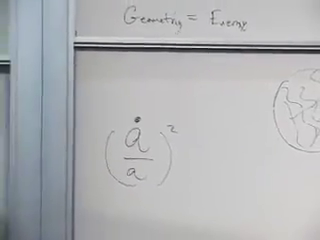
\includegraphics[width=0.68\textwidth]{lecture_06_figure_03.png}
\lectureframe{01:06:37.088}
\caption{Организующий лозунг \emph{геометрия равна энергии}, а под ним записан член расширения \(H^2=(\dot a/a)^2\).}
\end{figure}

Для однородной и изотропной Вселенной первое уравнение Фридмана имеет вид
\begin{equation}
H^2+\frac{k}{a^2}
=\frac{8\pi G}{3}\rho,
\end{equation}
в единицах \(c=1\), где \(k=+1,0,-1\) обозначает соответственно замкнутую, плоскую или открытую пространственную геометрию, а полная плотность энергии равна
\begin{equation}
\rho
=\rho_{\mathrm{ordinary}}
+\rho_{\mathrm{dark}}
+\rho_{\mathrm{radiation}}
+\rho_{\mathrm{vacuum}}.
\end{equation}
Знак, стоящий рядом с \(1/a^2\), зависит от того, оставляют ли член кривизны слева или переносят вправо, а также от значения \(k\).

\begin{figure}[H]
\centering
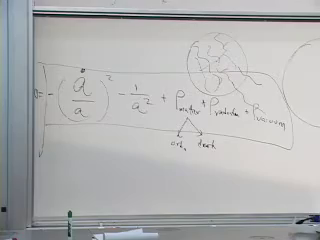
\includegraphics[width=0.96\textwidth]{lecture_06_figure_04.png}
\lectureframe{01:08:46.794}
\caption{Полный баланс на доске: расширение и пространственная кривизна на геометрической стороне, а вещество, излучение и вакуумная энергия — на стороне источников. Вещество далее разделено на обычную и тёмную компоненты.}
\end{figure}

\subsection{Космологическое гамильтоново ограничение}

\begin{classroomqa}
\audiencequestion{Если вакуумная энергия в сопутствующей области растёт по мере расширения Вселенной, существует ли тогда постоянная суммарная плотность энергии или сохраняется полная энергия? \lecturetimestamp{01:01:51}}
\lecturerresponse{Общая теория относительности не задаёт универсальной глобальной энергии для произвольного расширяющегося пространства-времени. Однако в однородной космологической редукции уравнение Эйнштейна для компоненты время–время является гамильтоновым ограничением. Если геометрические и материальные члены собрать в одной части уравнения, гамильтониан с ограничением обращается в нуль. Меняющиеся члены материи уравновешиваются гравитационными степенями свободы, а не обычной фиксированной энергией в ящике.}
\end{classroomqa}

Схематически каноническое утверждение имеет вид
\begin{equation}
\mathcal H_{\mathrm{gravity}}
+\mathcal H_{\mathrm{matter}}
=0.
\end{equation}
Именно в этом состоит точный смысл утверждения, что полная энергия равна нулю. Это уравнение движения, навязываемое инвариантностью относительно перепараметризации времени, а не утверждение о том, что всякая локальная плотность энергии обращается в нуль. В сопутствующем объёме энергия обычного вещества приблизительно постоянна, энергия излучения уменьшается, а вакуумная энергия растёт; тем временем гравитационный вклад и скорость расширения подстраиваются так, чтобы ограничение Эйнштейна продолжало выполняться.

Локальное сохранение остаётся точным:
\begin{equation}
\nabla_\mu T^{\mu\nu}=0.
\end{equation}
Для однородного флюида это в точности уравнение непрерывности \(\dot\rho+3H(\rho+p)=0\). Обычно неверна интуиция плоского пространства-времени, согласно которой в расширяющейся Вселенной должна существовать и одна координатно-независимая глобальная сумма энергии материи, сохраняющаяся во времени.\editorialnote{Это различие делает точным утверждение, прозвучавшее на лекции, что энергия всегда равна нулю: локальное ковариантное сохранение и космологическое гамильтоново ограничение точны, тогда как однозначно определённая глобальная энергия материи и гравитации, вообще говоря, не определена.}

\begin{classroomqa}
\audiencequestion{Является ли нулевое ограничение условием, определяющим, открыта Вселенная, замкнута или плоска? \lecturetimestamp{01:04:42}}
\lecturerresponse{Нет. Гамильтоново ограничение действует во всех случаях. Открытые, плоские и замкнутые вселенные различаются меткой кривизны \(k\) и, следовательно, членом \(k/a^2\). Кривизна изменяет один из вкладов в баланс; она не включает и не выключает ограничение.}
\end{classroomqa}

\section{Координаты Грассмана и суперполя}

\begin{classroomqa}
\audiencequestion{Возникают ли числа Грассмана непосредственно в лагранжиане теории? \lecturetimestamp{01:09:37}}
\lecturerresponse{Сначала они возникают потому, что фермионные поля грассманово нечётны. Затем — как координаты суперпространства. Суперполя зависят от этих нечётных координат, а суперсимметричные действия строятся дифференцированием и интегрированием по ним.}
\end{classroomqa}

Обычное поле является функцией пространства-времени,
\begin{equation}
\phi=\phi(x^\mu).
\end{equation}
Минимальная суперсимметрия в четырёх измерениях дополняет \(x^\mu\) двухкомпонентным нечётным спинором \(\theta^\alpha\) и сопряжённым к нему \(\bar\theta^{\dot\alpha}\):
\begin{equation}
z^M=(x^\mu,\theta^\alpha,\bar\theta^{\dot\alpha}).
\end{equation}
Имеются две комплексные нечётные компоненты, или 4 вещественных нечётных направления. Суперполе — это функция на этом суперпространстве:
\begin{equation}
\Phi=\Phi(x,\theta,\bar\theta).
\end{equation}

Это не крошечные пространственные измерения в метрическом смысле. Координата Грассмана не имеет положительной численной величины. Называть её малой — лишь мнемоника для нильпотентности:
\begin{equation}
(\theta^\alpha)^2=0,
\qquad
\theta^\alpha\theta^\beta=-\theta^\beta\theta^\alpha.
\end{equation}
\editorialnote{Именно нильпотентность, а не численная малость, является причиной того, что всякое разложение по конечному числу координат Грассмана обрывается.}

С четырьмя независимыми нечетными координатами совершенно общее суперполе содержит не более \(2^4=16\) грассмановых мономов. Схематически,
\begin{equation}
\begin{aligned}
\Phi(x,\Theta)={}&\phi(x)+\Theta_A\psi_A(x)\\
&+\frac{1}{2}\Theta_A\Theta_B Z_{AB}(x)+\cdots\\
&+\Theta_1\Theta_2\Theta_3\Theta_4D(x),
\end{aligned}
\end{equation}
где \(\Theta_A\) совместно обозначает четыре вещественные нечетные координаты. Поскольку всё суперполе можно выбрать чётным, коэффициенты при мономах чётной степени являются бозонными, а коэффициенты при мономах нечётной степени — фермионными. Поэтому одно суперполе объединяет конечный мультиплет обычных компонентных полей.

Такое объединение — больше, чем просто обозначение. Суперсимметрия действует геометрически как трансляция по нечетным направлениям, смешанная с трансляцией в пространстве-времени. Лагранжиан, построенный из суперполей по правилам суперпространства, наследует эту симметрию точно так же, как скалярный лагранжиан, построенный из тензоров, наследует инвариантность относительно вращений или преобразований Лоренца.

В действие теперь входят грассмановы меры. Типичный член с мерой полного суперпространства имеет вид
\begin{equation}
S_D=\int d^4x\,d^2\theta\,d^2\bar\theta\,
\mathcal K(\Phi,\Phi^\dagger).
\end{equation}
Для хиральных членов вместо этого используется
\begin{equation}
S_F=\int d^4x\,d^2\theta\,W(\Phi)+\mathrm{h.c.}
\end{equation}
\editorialnote{Различие между мерой полного суперпространства и хиральной мерой — это стандартное уточнение схематического действия \(d^4x\,d^4\theta\). На конкретных примерах будет ясно, какая мера подходит.}

Тем самым мы подошли к вопросу, на который обычный анализ не отвечает: что означает интегрирование по антикоммутирующей координате?

\section{Интегрирование Березина}

\subsection{Обычная модель: полная производная}

Начнём с обычной функции \(F(x)\), которая обращается в нуль при больших положительных и отрицательных значениях \(x\). Основная теорема анализа даёт
\begin{equation}
\int_{-\infty}^{\infty}dx\,\frac{dF}{dx}
=F(\infty)-F(-\infty)
=0.
\end{equation}

\begin{figure}[H]
\centering
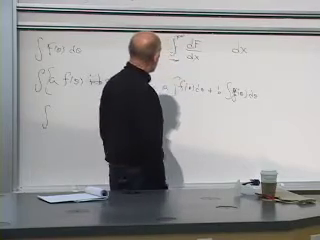
\includegraphics[width=0.88\textwidth]{lecture_06_figure_05.png}
\lectureframe{01:26:31.594}
\caption{Обычный прототип интегрирования Березина: интеграл от полной производной сводится к значениям на концах и обращается в нуль, когда функция затухает. Нижняя строка на доске частично закрыта, поэтому аккуратное уравнение приведено в тексте.}
\end{figure}

Мы хотим, чтобы интеграл по грассмановой переменной был линейным и обладал полезным свойством: интеграл от полной производной равен нулю. Для одной нечетной координаты потребуем
\begin{align}
\int d\theta\,[af(\theta)+bg(\theta)]
&=
a\int d\theta\,f(\theta)
+b\int d\theta\,g(\theta),\\
\int d\theta\,\partial_\theta f(\theta)&=0.
\end{align}
Второе условие — алгебраический аналог трансляционной инвариантности меры. У числовой прямой для нечетной координаты нет концов и нет суммирования по малым интервалам.

\begin{classroomqa}
\audiencequestion{Если неопределённого интеграла по грассмановой переменной нет, отказываемся ли мы тогда от идеи, что интегрирование является обратной операцией к дифференцированию? \lecturetimestamp{01:21:19}}
\lecturerresponse{Да. Интегрирование Березина — это определённый линейный функционал, а не операция взятия первообразной. Для одной грассмановой переменной оно фактически задаётся той же алгебраической операцией, что и дифференцирование.}
\end{classroomqa}

\begin{classroomqa}
\audiencequestion{Является ли интегрирование \(d^4x\) по всему пространству-времени тоже определённым интегралом? \lecturetimestamp{01:21:34}}
\lecturerresponse{Да. При интегрировании действия по пространству-времени граничные условия подразумеваются. Разница в том, что обычное интегрирование по пространству-времени можно понимать как предел сумм, тогда как грассманово интегрирование определяется алгебраически своим действием на конечный базис \(1,\theta\).}
\end{classroomqa}

\subsection{Одна переменная}

Любую функцию одной нечетной переменной можно записать так, чтобы коэффициент стоял справа, в фиксированном порядке,
\begin{equation}
f(\theta)=a+\theta b.
\end{equation}
Поскольку \(\partial_\theta\theta=1\), из правила для полной производной следует
\begin{equation}
\int d\theta\,1=0.
\end{equation}
Оставшуюся нормировку выбирают равной
\begin{equation}
\int d\theta\,\theta=1.
\end{equation}
Следовательно,
\begin{equation}
\int d\theta\,f(\theta)=b.
\end{equation}
Интеграл выделяет коэффициент при наивысшей возможной степени. При используемом здесь соглашении о левой производной
\begin{equation}
\partial_\theta f=b
=\int d\theta\,f.
\end{equation}

\begin{classroomqa}
\audiencequestion{Существует ли функция \(F(\theta)\), удовлетворяющая условию \(\partial_\theta F=\theta\)? \lecturetimestamp{01:30:05}}
\lecturerresponse{Нет. Такой функции понадобился бы член, пропорциональный \(\theta^2\), но \(\theta^2=0\). Это ещё один способ увидеть, почему не существует грассманова аналога неопределённой первообразной.}
\end{classroomqa}

\subsection{Две переменные и порядок меры}

Для комплексной пары \(\theta,\bar\theta\) запишем общую чётную функцию в упорядоченной форме
\begin{equation}
f(\theta,\bar\theta)
=a+\bar\theta\psi+\bar\psi\theta+b\,\bar\theta\theta.
\end{equation}
Членов более высокой степени нет, поскольку
\begin{equation}
\theta^2=\bar\theta^2=0,
\qquad
\bar\theta\theta=-\theta\bar\theta.
\end{equation}

Теперь зафиксируем соглашение
\begin{equation}
\int d\theta\,d\bar\theta\,
\bar\theta\theta=1.
\end{equation}
В повторных интегралах первой действует соседняя операция \(d\bar\theta\). Тогда таблица такова:
\begin{align}
\int d\theta\,d\bar\theta\,1&=0,\\
\int d\theta\,d\bar\theta\,\theta&=0,\\
\int d\theta\,d\bar\theta\,\bar\theta&=0,\\
\int d\theta\,d\bar\theta\,\bar\theta\theta&=1.
\end{align}
Тем самым
\begin{equation}
\int d\theta\,d\bar\theta\,
f(\theta,\bar\theta)=b.
\end{equation}

\begin{classroomqa}
\audiencequestion{Для члена, линейного по \(\theta\), неужели именно интегрирование по \(\theta\) обращает двойной интеграл в нуль? \lecturetimestamp{01:34:59}}
\lecturerresponse{Нет; в устном объяснении роли были перепутаны. Интегрирование \(\theta\) по \(\theta\) даёт единицу. Тогда результат уже не содержит \(\bar\theta\), и оставшийся интеграл по \(\bar\theta\) от единицы равен нулю. В любом случае двойной интеграл даёт ненулевой результат только тогда, когда присутствуют обе переменные.}
\end{classroomqa}

\begin{classroomqa}
\audiencequestion{Если \(\theta\) и \(\bar\theta\) переставить, меняет ли интеграл знак? \lecturetimestamp{01:36:33}}
\lecturerresponse{Да. Нечётные переменные и нечётные меры антикоммутируют. При соглашении выше
\[
\int d\bar\theta\,d\theta\,\bar\theta\theta=-1.
\]
Поэтому нужно выбрать порядок и затем последовательно его сохранять. Физика не зависит от соглашения, но промежуточные знаки зависят.}
\end{classroomqa}

Для \(n\) независимых грассмановых переменных схема сразу ясна:
\begin{equation}
\int d\theta_n\cdots d\theta_1\,
f(\theta_1,\ldots,\theta_n)
\end{equation}
выделяет коэффициент при упорядоченном старшем мономе \(\theta_1\cdots\theta_n\) с точностью до знака, фиксированного выбранным порядком переменных и мер. Это простое правило выделения компонент лежит в основе действий в суперпространстве. Вариация суперсимметрии превращается в нечётную полную производную, и интеграл по суперпространству отбрасывает её, точно так же как обычное действие отбрасывает полную производную по пространству-времени при подходящих граничных условиях.

\section{Почему столь малое исчисление обладает такой силой}

Правила выглядят почти тривиально:
\begin{equation}
\int d\theta\,1=0,
\qquad
\int d\theta\,\theta=1.
\end{equation}
И всё же они позволяют строить теории поля с взаимодействием, в которых соотношения между бозонными и фермионными массами и константами связи автоматически сохраняются. Назначение исчисления суперпространства то же, что и назначение тензорного исчисления в теории относительности: организовать обозначения так, чтобы нужная симметрия сохранялась при любых допустимых манипуляциях.

Ценой за это является тщательный учёт знаков. Каждая перестановка двух нечётных объектов вносит минус, и вычисление может быть концептуально правильным, но дать сбой из-за одного выбора порядка. Эта трудность не декоративна; это алгебраическая тень фермионной статистики.

\begin{classroomqa}
\audiencequestion{Числа Грассмана были введены вместе с суперсимметрией или существовали раньше? \lecturetimestamp{01:41:19}}
\lecturerresponse{Они намного старше. Герман Грассман разработал лежащую в основе внешнюю алгебру в XIX веке. В дифференциальных формах уже используются антикоммутирующие базисные элементы; квантовая теория поля XX века и суперсимметрия нашли для той же математики новую физическую роль.}
\end{classroomqa}

Теперь мы готовы к конкретным построениям. Суперполя собирают полные бозон-фермионные мультиплеты, производные в суперпространстве сохраняют алгебру, а интегрирование Березина извлекает компонентное действие. Следующая задача — применить этот аппарат в простейшей одномерной модели, а затем перенести его в теорию поля.

\chapter{Суперпространство и построение суперсимметричной динамики}

\lectureoverview{Мы заново строим суперсимметрию, начиная с наименьшей системы, в которой она может действовать: одного бозонного осциллятора и одного фермионного осциллятора с одинаковой энергией. Контраст между их уравнениями второго и первого порядка приводит к суперзарядам и их алгебре. Затем мы переинтерпретируем эту алгебру как геометрию на пространстве с обычной координатой (t) и грассмановыми координатами \(\theta,\bar\theta\). Суперполя объединяют бозоны, фермионы и вспомогательное поле в один объект; интегрирование Березина выделяет инвариантный обычный лагранжиан; ковариантные производные делают возможными ограничения, совместимые с симметрией; а киральное ограничение даёт первый важный пример. На лекции намеренно вскрываются трудности со знаками и порядком множителей в этом аппарате, а в заключение объясняется, почему сама симметрия более фундаментальна, чем перечень правил Фейнмана.}

\section{Возвращение к одномодовой системе}

Начнём снова с фермионов и бозонов в покое. Мы опускаем все пространственные координаты и все метки импульса. В данной моде квант либо присутствует, либо отсутствует, и для его описания достаточно операторов рождения и уничтожения. Обозначим бозонную моду через \(a^\dagger,a\), а фермионную — через \(c^\dagger,c\). Они удовлетворяют соотношениям
\begin{align}
[a,a^\dagger]&=1,
&
\{c,c^\dagger\}&=1,
&
c^2=(c^\dagger)^2&=0.
\end{align}
Если оба кванта имеют одинаковую энергию \(m\), то с точностью до несущественной вакуумной константы
\begin{equation}
H=m\left(a^\dagger a+c^\dagger c\right).
\label{eq:l7-one-mode-hamiltonian}
\end{equation}
Оператор числа \(a^\dagger a\) может принимать любые неотрицательные целые значения, тогда как \(c^\dagger c\) — только 0 или 1. Это и есть вся кинематика этой игрушечной модели.

Это упрощение стратегично. Мы хотим понять операцию, которая уничтожает бозон и создаёт фермион, или делает обратное, не изменяя энергии. Однако прежде чем строить эту операцию, переведём ту же систему с операторного языка на язык лагранжиана.

\section{Бозонный осциллятор}

Для бозона введём вещественную координату \(\phi(t)\). При отсутствии пространственной зависимости свободное скалярное поле превращается в обычный гармонический осциллятор. Первое выражение, написанное на доске, было
\[
\frac{1}{2}\dot\phi^{,2}+\frac{1}{2}m^2\phi^2.
\]
Это выражение есть сумма кинетической и потенциальной энергий, а не лагранжиан. На лекции знак сразу же исправляется:
\begin{equation}
L_B=\frac{1}{2}\dot\phi^{,2}-\frac{1}{2}m^2\phi^2.
\label{eq:l7-boson-lagrangian}
\end{equation}

\begin{figure}[H]
\centering
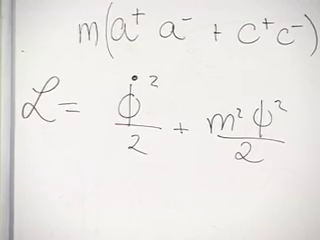
\includegraphics[width=0.62\textwidth]{lecture_07_figure_02.png}
\lectureframe{00:03:25.431}
\caption{Одномодовый гамильтониан над бозонным лагранжианом. На кадре сохранён исходный знак плюс до устного исправления на \(T-V\).}
\end{figure}

\begin{classroomqa}
\audiencequestion{Что не так со знаком в выписанном лагранжиане осциллятора? \lecturetimestamp{00:04:00}}
\lecturerresponse{Энергия равна \(T+V\), а лагранжиан — \(T-V\). Поэтому потенциальный член должен входить с минусом. Исправление меняет уравнение так, что вместо экспоненциального поведения получаются ожидаемые гармонические колебания.}
\end{classroomqa}

Действительно, уравнение Эйлера--Лагранжа даёт
\begin{align}
\frac{d}{dt}\frac{\partial L_B}{\partial\dot\phi}
&=\frac{\partial L_B}{\partial\phi},\\
\ddot\phi&=-m^2\phi,
\end{align}
или
\begin{equation}
\ddot\phi+m^2\phi=0.
\label{eq:l7-boson-eom}
\end{equation}
Его частота равна \(m\), а не \(m^2\). Квантование этого осциллятора воспроизводит ту же лестницу состояний, которая описывается \(a^\dagger\) и \(a\) в уравнении~\eqref{eq:l7-one-mode-hamiltonian}.

\section{Почему фермионное действие имеет первый порядок}

Фермионный лагранжиан выглядит проще, потому что содержит только одну производную по времени. Причина уже видна в намеренно наивной пробе. Для обычной коммутирующей переменной
\begin{equation}
L_{\mathrm{trial}}=\phi\dot\phi
=\frac{1}{2}\frac{d}{dt}\phi^2.
\end{equation}
это полная производная. Соответствующее уравнение Эйлера--Лагранжа утверждает лишь \(\dot\phi=\dot\phi\), так что допустим любой дифференцируемый путь. Вычитание полной производной из действия меняет граничные данные, но не внутреннее уравнение движения.

Теперь переименуем переменную в \(\psi\) и объявим её грассманово нечётной. И \(\psi\), и \(\dot\psi\) антикоммутируют. При фиксированном выборе левой вариации перестановка нечётных множителей вносит минус, так что та же формальная проба даёт
\begin{equation}
\frac{d}{dt}\frac{\partial L_{\mathrm{trial}}}{\partial\dot\psi}
=\dot\psi,
\qquad
\frac{\partial L_{\mathrm{trial}}}{\partial\psi}
=-\dot\psi.
\end{equation}
Следовательно, уравнение имеет вид
\begin{equation}
\dot\psi=-\dot\psi
\quad\Longrightarrow\quad
\dot\psi=0.
\label{eq:l7-constant-fermion}
\end{equation}
Выражение, которое для коммутирующей координаты было тавтологией, для антикоммутирующей приобрело динамическое содержание. Для осциллятора это условие слишком жёстко, поскольку допускает только константу, но именно эта подсказка нам и нужна.

\begin{classroomqa}
\audiencequestion{Неужели решение просто в том, что \(\psi\) — константа? \lecturetimestamp{00:13:57}}
\lecturerresponse{Да. Уравнение~\eqref{eq:l7-constant-fermion} — это настоящее дифференциальное уравнение первого порядка, и его решением служит произвольная грассманнозначная константа. Массовый член превратит это статическое решение в осциллирующее.}
\end{classroomqa}

Очевидная попытка, \(m\psi^2\), не проходит, потому что \(\psi^2=0\). Нужны две вещественные нечётные переменные \(\psi_1,\psi_2\), или, что эквивалентно, одна комплексная переменная и её сопряжённая. На лекции на доске разбирается форма с двумя вещественными переменными, с многократной проверкой знаков и множителей 2. При обычной нормировке комплексная форма имеет вид
\begin{equation}
L_F=\frac{i}{2}
\left(\bar\psi\dot\psi-\dot{\bar\psi}\psi\right)
-m\bar\psi\psi.
\label{eq:l7-fermion-lagrangian}
\end{equation}
С точностью до полной производной это \(i\bar\psi\dot\psi-m\bar\psi\psi\). Варьирование по \(\bar\psi\) даёт
\begin{equation}
i\dot\psi=m\psi,
\qquad
\psi(t)=\psi(0)e^{-imt}.
\label{eq:l7-fermion-eom}
\end{equation}
Сопряжённое уравнение имеет противоположную фазу. Таким образом, фермионная мода осциллирует с энергией \(m\), как и бозонная, хотя её уравнение первого, а не второго порядка.

\editorialnote{Формула~\eqref{eq:l7-fermion-lagrangian} фиксирует один стандартный порядок множителей и нормировку для пробного расчёта с двумя вещественными переменными. На самой лекции вводится множитель \(i\), подправляется множитель 2, и знак у одной вещественной компоненты остаётся неуточнённым. Эти изменения не меняют главного вывода: кинетический член фермиона имеет первый порядок, масса входит линейно, а комплексный фермион даёт ненулевую билинейную комбинацию.}

Это нульмерная тень знакомого релятивистского контраста. Уравнение Клейна--Гордона имеет второй порядок по времени, тогда как уравнение Дирака — первый. При опущенной пространственной зависимости бозон — это один гармонический осциллятор, а фермион — один комплексный грассмановский осциллятор.

\begin{classroomqa}
\audiencequestion{Имеет ли значение порядок, в котором записываются \(\psi\), \(\dot\psi\) и их сопряжённые? \lecturetimestamp{00:18:58}}
\lecturerresponse{Промежуточные формулы действительно зависят от порядка, потому что нечётные множители антикоммутируют. Физическая теория не зависит от произвольного предпочтения в записи, если повсюду последовательно использовать одну и ту же конвенцию для левой или правой вариации, сопряжения и интегрирования. Перестановка нечётной пары меняет знак, и тогда его нужно везде последовательно изменить.}
\end{classroomqa}

Объединяя уравнения~\eqref{eq:l7-boson-lagrangian} и \eqref{eq:l7-fermion-lagrangian}, мы получаем лагранжево описание той же пары, которая представлена уравнением~\eqref{eq:l7-one-mode-hamiltonian}. Теперь мы готовы выделить симметрию между ними.

\section{Суперзаряды и их алгебра}

Оператор, который уничтожает фермион и создаёт бозон, имеет вид
\begin{equation}
Q^\dagger=\sqrt{2m}\,a^\dagger c,
\end{equation}
тогда как его сопряжённый уничтожает бозон и создаёт фермион,
\begin{equation}
Q=\sqrt{2m}\,a c^\dagger.
\end{equation}
Нормировка выбрана так, чтобы алгебра принимала стандартный вид. Используя \(cc^\dagger=1-c^\dagger c\), \(aa^\dagger=a^\dagger a+1\) и тот факт, что бозонные и фермионные операторы коммутируют друг с другом,
\begin{align}
\{Q,Q^\dagger\}
&=2m\left(ac^\dagger a^\dagger c+a^\dagger c a c^\dagger\right)\notag\\
&=2m\left[(a^\dagger a+1)c^\dagger c
+a^\dagger a(1-c^\dagger c)\right]\notag\\
&=2m\left(a^\dagger a+c^\dagger c\right)=2H.
\label{eq:l7-superalgebra}
\end{align}
Бозонные операторы можно переносить через фермионные. Та же нильпотентность, которая ограничивает заполнение фермионной моды, даёт
\begin{equation}
Q^2=(Q^\dagger)^2=0.
\end{equation}
Наконец,
\begin{equation}
[H,Q]=[H,Q^\dagger]=0.
\label{eq:l7-conserved-supercharges}
\end{equation}
Каждый суперзаряд изменяет число бозонов и число фермионов в противоположных направлениях, так что при равных частотах два изменения энергии компенсируют друг друга.

\begin{classroomqa}
\audiencequestion{Чему равно \([H,Q]\)? Пропорционален ли ответ \(Q\)? \lecturetimestamp{00:25:10}}
\lecturerresponse{Нет. Ответ равен нулю. Отдельный оператор рождения или уничтожения при коммутировании с \(H\) получил бы множитель, равный своей энергии, но бозонный и фермионный вклады в \(Q\) сокращаются. Именно это сокращение и выражает условие равенства энергий.}
\end{classroomqa}

\begin{classroomqa}
\audiencequestion{Разве этот коммутатор уже не был написан на доске? \lecturetimestamp{00:25:45}}
\lecturerresponse{Был. Повторное получение полезно, потому что заставляет нас не просто переписать это соотношение, а интерпретировать его: коммутирование с гамильтонианом означает, что преобразование является симметрией и что его генератор сохраняется.}
\end{classroomqa}

Слово \emph{заряд} отражает этот закон сохранения. Однако не следует рассматривать \(Q\) как обычное совместно измеримое число, приписанное состоянию. Он грассманово нечётен, нильпотентен и переводит бозонное состояние в фермионное. Содержательное утверждение состоит в том, что это сохраняющийся генератор, действующий внутри вырожденных супермультиплетов.
\editorialnote{Эта формулировка уточняет использованную в аудитории аналогию с маркировкой состояний по энергии или электрическому заряду. Отдельные неэрмитовы нечётные суперзаряды не являются обычными наблюдаемыми с числовыми квантовыми метками. Их сохраняющееся действие и представление полной супералгебры дают правильную классификацию.}

\section{Генераторы как производные}

Алгебра компактна, но сама по себе она не говорит нам, как строить теории с взаимодействием. Следующий шаг — геометрический. Знакомые генераторы симметрий уже действуют как дифференциальные операторы. В соглашении, принятом на лекции,
\begin{equation}
H=i\frac{\partial}{\partial t},
\qquad
P=-i\frac{\partial}{\partial x}.
\end{equation}

\begin{figure}[H]
\centering
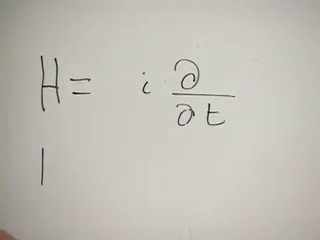
\includegraphics[width=0.50\textwidth]{lecture_07_figure_03.png}
\lectureframe{00:28:12.720}
\caption{Гамильтониан, представленный как генератор временных трансляций.}
\end{figure}

Угловой момент аналогично представляет собой координату, умноженную на производную. Если суперзаряды являются нечётными генераторами, естественно спросить, можно ли представить их производными по нечётным координатам. Поэтому мы расширяем ось времени до суперпространства
\begin{equation}
(t,\theta,\bar\theta),
\qquad
\theta^2=\bar\theta^2=0,
\qquad
\theta\bar\theta=-\bar\theta\theta.
\end{equation}
Поля на этом пространстве зависят от обычного времени и сопряжённой пары грассмановых координат.

Лекция намеренно показывает, насколько коварны знаки. Знак, возникающий при комплексном сопряжении, знак, возникающий при перестановке нечётного параметра, и знак, связанный с выбором левых, а не правых производных, соответствуют разным операциям. Вместо того чтобы сохранять взаимно несовместимые этапы выкладок на доске, мы теперь фиксируем одно соглашение: все нечётные производные являются левыми, и
\begin{equation}
q=\partial_\theta+i\bar\theta\partial_t,
\qquad
\bar q=\partial_{\bar\theta}+i\theta\partial_t.
\label{eq:l7-differential-supercharges}
\end{equation}
Тогда
\begin{equation}
q^2=\bar q^{,2}=0,
\qquad
\{q,\bar q\}=2i\partial_t=2H.
\label{eq:l7-differential-algebra}
\end{equation}
Коэффициент 2 возникает из двух перекрёстных членов: \(\{\partial_\theta,\theta\}=1\) и \(\{\partial_{\bar\theta},\bar\theta\}=1\). Если бы генераторы содержали только \(\partial_\theta\) и \(\partial_{\bar\theta}\), их антикоммутатор обращался бы в нуль и не мог бы воспроизвести гамильтониан.

\begin{classroomqa}
\audiencequestion{Должны ли два члена с производной по времени в \(q\) и \(\bar q\) иметь один и тот же знак? \lecturetimestamp{00:31:01}}
\lecturerresponse{Их нужно выбирать согласованно, так чтобы смешанный антикоммутатор был \(2H\). Можно использовать либо соглашение с общим плюсом, либо его согласованно сопряжённую альтернативу. Относительные знаки определяются вычислением, а не зрительной интуицией относительно символа \(i\).}
\end{classroomqa}

Аудитория снова и снова проверяет знаки, и трудность превращается в шутку: кажется, будто по дороге на работу знаки успевают измениться. Шутка уместна. Если антикоммутировать грассманов параметр с координатой, знак может измениться, даже когда никакое физическое соглашение не менялось. Уравнение~\eqref{eq:l7-differential-supercharges} служит фиксированной точкой отсчёта для всего последующего.

\subsection{Суперсимметрия как сдвиг координат}

Пусть \(\xi,\bar\xi\) — бесконечно малые нечётные параметры. Действие на суперполе посредством
\begin{equation}
\delta_\xi=\xi q+\bar\xi\bar q
\end{equation}
эквивалентно в приведённом выше соглашении бесконечно малому преобразованию координат
\begin{align}
\theta&\longrightarrow\theta+\xi,\\
\bar\theta&\longrightarrow\bar\theta+\bar\xi,\\
t&\longrightarrow t+i\left(\xi\bar\theta+\bar\xi\theta\right).
\label{eq:l7-coordinate-shift}
\end{align}
Поэтому изменение скалярного суперполя равно
\begin{equation}
\delta_\xi\Phi
=\left(\xi\partial_\theta+\bar\xi\partial_{\bar\theta}
+i\xi\bar\theta\partial_t+i\bar\xi\theta\partial_t\right)\Phi
=\left(\xi q+\bar\xi\bar q\right)\Phi.
\end{equation}
В этом состоит геометрическое содержание суперсимметрии. Это сдвиг по нечётным направлениям, связанный со сдвигом по обычному времени. Два нечётных сдвига замыкаются на сдвиг по времени в силу уравнения~\eqref{eq:l7-differential-algebra}.

\begin{classroomqa}
\audiencequestion{Может ли спорный минус означать движение назад во времени? \lecturetimestamp{00:58:13}}
\lecturerresponse{Иное соглашение о знаках может обратить показанный бесконечно малый сдвиг по времени, но никакой отдельный физический процесс обратного хода времени при этом не вводится. Важно то, что преобразование координат и дифференциальные генераторы подчиняются одной и той же алгебре.}
\end{classroomqa}

\begin{classroomqa}
\audiencequestion{Имеет ли это расширенное время физическую реализацию, или это лишь формальное средство учёта? \lecturetimestamp{00:58:23}}
\lecturerresponse{В одном полезном смысле это действительно средство учёта: оно упаковывает алгебру в геометрию. Но такая упаковка становится физически ценной, когда вводятся взаимодействия. Суперпространство даёт систематическое исчисление для построения лагранжианов, сохраняющих бозон--фермионную симметрию на каждом шаге, точно так же, как тензорное исчисление помогает нам строить скаляры Лоренца.}
\end{classroomqa}

\section{Суперполя и вспомогательная компонента}

Поскольку нечётных координат всего две, разложение чётного суперполя обрывается:
\begin{equation}
\Phi(t,\theta,\bar\theta)
=\phi(t)+\bar\theta\psi(t)+\bar\psi(t)\theta
+D(t)\bar\theta\theta.
\label{eq:l7-superfield}
\end{equation}
Коэффициенты при чётных мономах, \(\phi\) и \(D\), являются бозонными; коэффициенты при нечётных мономах, \(\psi\) и \(\bar\psi\), являются фермионными. Никакой член с \(\theta^2\), \(\bar\theta^2\) или более высокой степенью не остаётся. Зависимость от времени мы не раскладываем, потому что обычный ряд Тейлора по \(t\) не обрывался бы и здесь не служил бы никакой цели.

\begin{classroomqa}
\audiencequestion{Что представляет собой компонента \(D(t)\) в старшем члене? \lecturetimestamp{00:41:46}}
\lecturerresponse{На этом этапе это просто последний бозонный коэффициент в конечном разложении. В компонентном действии у него обычно нет кинетического члена, и он устраняется алгебраическим уравнением движения, поэтому его называют вспомогательным полем. Лектор шутливо предлагает ``D для dummy,'' что передаёт его нединамическую роль, не являясь при этом историческим определением.}
\end{classroomqa}

Суперполе — это один объект, тогда как \(\phi,\psi,\bar\psi,D\) — его компоненты. Преобразование суперсимметрии перемешивает их. Поэтому бозон и фермион связаны примерно в том же структурном смысле, в каком \(x\)- и \(y\)-компоненты вектора связаны поворотом, хотя грассмановы направления нельзя изобразить как обычные оси.

\section{Супердействие и старшая компонента}

Чтобы получить уравнения движения, нам нужно действие. В обычной теории поля строят скалярный лагранжиан и интегрируют его по пространству-времени. Здесь аналогичное выражение имеет вид
\begin{equation}
S=\int dt\,d\theta\,d\bar\theta\;\Lambda
\bigl(\Phi,\text{ superspace derivatives of }\Phi\bigr),
\label{eq:l7-superaction}
\end{equation}
где \(\Lambda\) — чётное суперполе. Интегрирование Березина алгебраично. Мы выбираем
\begin{equation}
\int d\theta\,d\bar\theta\;\bar\theta\theta=1.
\end{equation}
Следовательно, если
\begin{equation}
\Lambda=A+\bar\theta B+\bar B\theta+C\bar\theta\theta,
\end{equation}
то
\begin{equation}
\int d\theta\,d\bar\theta\;\Lambda=C.
\label{eq:l7-top-component}
\end{equation}
Интеграл по нечётным координатам выделяет старшую компоненту, оставляя обычный лагранжиан, который затем интегрируется по времени.

Почему результат инвариантен? Вариация суперсимметрии сдвигает переменные интегрирования. Вариация старшей компоненты есть обычная полная производная по времени, тогда как полные производные по нечётным координатам исчезают при интегрировании Березина. При подходящих граничных условиях действие не изменяется. Это суперпространственный аналог построения скаляра Лоренца перед его интегрированием по пространству-времени.

\section{Умножение суперполей}

Самый простой способ получить новое суперполе из старого — умножить его само на себя. Исходя из уравнения~\eqref{eq:l7-superfield}, каждый член, содержащий \(\theta^2\) или \(\bar\theta^2\), обращается в нуль. Сохраняя порядок \(\bar\theta\theta\) и записывая компоненты с чертой слева, получаем
\begin{align}
\Phi^2
={}&\phi^2
+2\phi\bar\theta\psi
+2\phi\bar\psi\theta\notag\\
&+\left(2\phi D-2\bar\psi\psi\right)\bar\theta\theta.
\label{eq:l7-superfield-square}
\end{align}

\begin{figure}[H]
\centering
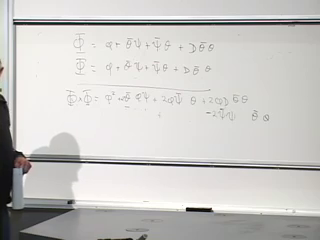
\includegraphics[width=0.82\textwidth]{lecture_07_figure_05.png}
\lectureframe{01:07:57.844}
\caption{Покомпонентное произведение суперполя и сбор всех его членов с \(\bar\theta\theta\).}
\end{figure}

Два члена \(\phi D\) и \(D\phi\) складываются, потому что оба поля чётные. Два перекрёстных фермионных члена тоже складываются после того, как каждый из них переставлен, но их общий знак отрицателен:
\begin{equation}
(\bar\theta\psi)(\bar\psi\theta)
+(\bar\psi\theta)(\bar\theta\psi)
=-2\bar\psi\psi\,\bar\theta\theta.
\end{equation}
Интегрируя квадрат по нечётным координатам, получаем
\begin{equation}
\int d\theta\,d\bar\theta\;\Phi^2
=2\phi D-2\bar\psi\psi.
\end{equation}
Этот член суперсимметричен по построению, но это ещё не кинетический лагранжиан. Он не содержит производных по времени.

Затем на доске в качестве упражнений предлагаются \(\Phi^3\), \(\Phi^4\) и \(\Phi^n\). Есть компактное правило. Для любой обычной функции \(W\),
\begin{equation}
\left.W(\Phi)\right|_{\bar\theta\theta}
=W'(\phi)D-W''(\phi)\bar\psi\psi.
\label{eq:l7-function-top-component}
\end{equation}
Для \(W(\phi)=\phi^2\) это воспроизводит уравнение~\eqref{eq:l7-superfield-square}; для \(W(\phi)=\phi^n\) получается
\begin{equation}
\left.\Phi^n\right|_{\bar\theta\theta}
=n\phi^{n-1}D-n(n-1)\phi^{n-2}\bar\psi\psi.
\end{equation}
\editorialnote{На лекции \(n\)-я степень предлагается как упражнение и перечисляются ожидаемые типы членов. Уравнение~\eqref{eq:l7-function-top-component} даёт полное правило в соглашении о фиксированном порядке.}

На этом месте лектор спрашивает, устала ли аудитория. Аудитория отвечает, что нет; он отвечает, что устал он. Этот обмен репликами — не просто комическая передышка. Степени суперполей просты, потому что разложение обрывается, но именно на производных и ограничениях учёт знаков становится по-настоящему трудным.

\section{Какие производные совместимы с суперсимметрией?}

Прежде чем переходить к следующему рассуждению на доске, нужно внести одну поправку. Обычная производная по времени безобидна:
\begin{equation}
[\partial_t,q]=[\partial_t,\bar q]=0.
\end{equation}
Следовательно, \(\partial_t\Phi\) преобразуется как суперполе всякий раз, когда так преобразуется \(\Phi\). Тонкость связана с самими нечётными производными \(\partial_\theta\Phi\) и \(\partial_{\bar\theta}\Phi\), потому что они не антикоммутируют с обоими суперзарядами. Для ограничений и для явно суперсимметричных компонентных построений нам нужны модифицированные нечётные производные.
\editorialnote{Устное утверждение о том, что дифференцирование по времени не даёт другого суперполя, неверно в используемом здесь соглашении. Поскольку \(\partial_t\) коммутирует с обоими суперзарядами, она ковариантна. Последующее построение модифицированных нечётных производных всё равно необходимо и составляет подлинную математическую суть лекции.}

\subsection{Аналогия с ``волшебным полем''}

Лекция мотивирует критерий на примере обычных поворотов. Пусть \(f(x,y)\) удовлетворяет условию
\begin{equation}
\partial_y f=0.
\label{eq:l7-magic-constraint}
\end{equation}
Назовём такую функцию ``волшебным полем''. Она зависит от \(x\), но не от \(y\). Сохраняется ли класс волшебных полей при поворотах? Для
\begin{equation}
L_z=-i\left(x\partial_y-y\partial_x\right),
\end{equation}
находим
\begin{equation}
[\partial_y,L_z]=i\partial_x\neq0.
\end{equation}
Следовательно, \(L_z f\), вообще говоря, приобретает зависимость от \(y\), даже когда \(f\) изначально удовлетворяет уравнению~\eqref{eq:l7-magic-constraint}. Это ограничение не инвариантно относительно поворотов.

Общий вывод прост. Если поле удовлетворяет \(C\Phi=0\) и симметрия порождается оператором \(G\), то преобразованное поле остаётся удовлетворяющим ограничению, когда градуированный коммутатор \(C\) и \(G\) равен нулю. Для двух нечётных операторов градуированный коммутатор есть антикоммутатор.

\begin{classroomqa}
\audiencequestion{Когда ограничение на поле совместимо с симметрией? \lecturetimestamp{01:17:56}}
\lecturerresponse{Когда оператор ограничения градуированно коммутирует с генераторами симметрии. Тогда \(C(G\Phi)\) можно перенести через \(G\) и свести к \(G(C\Phi)=0\). Пример с поворотом не работает, потому что \(\partial_y\) не коммутирует с генератором вращения.}
\end{classroomqa}

\subsection{Ковариантные нечётные производные}

Зафиксировав суперзаряды по уравнению ~\eqref{eq:l7-differential-supercharges}, определим
\begin{equation}
\mathcal D=\partial_\theta-i\bar\theta\partial_t,
\qquad
\bar{\mathcal D}=\partial_{\bar\theta}-i\theta\partial_t.
\label{eq:l7-covariant-derivatives}
\end{equation}
Единственное изменение — знак при члене с производной по времени. Прямое вычисление даёт
\begin{align}
\{\mathcal D,q\}
&=\{\mathcal D,\bar q\}
=\{\bar{\mathcal D},q\}
=\{\bar{\mathcal D},\bar q\}=0,\\
\{\mathcal D,\bar{\mathcal D}\}&=-2i\partial_t.
\label{eq:l7-covariant-algebra}
\end{align}
Два потенциально ненулевых перекрёстных члена сокращаются. Это нечётный аналог ковариантной производной: он дифференцирует, сохраняя закон преобразования.

В лекции обозначение \(D\) используется и для вспомогательной компоненты, и для этой производной. Для компоненты мы сохраняем \(D(t)\), а для оператора используем каллиграфическое \(\mathcal D\).

\section{Хиральное ограничение}

Теперь можно наложить нетривиальное ограничение, которое сохраняется при суперсимметрии:
\begin{equation}
\bar{\mathcal D}\Phi=0.
\label{eq:l7-chiral-constraint}
\end{equation}
Такое поле называется хиральным. Если до суперсимметричного преобразования оно хирально, то
\begin{equation}
\bar{\mathcal D}(q\Phi)
=-q(\bar{\mathcal D}\Phi)=0,
\qquad
\bar{\mathcal D}(\bar q\Phi)
=-\bar q(\bar{\mathcal D}\Phi)=0.
\end{equation}
Тем самым всё преобразованное суперполе остаётся внутри этого ограниченного класса. В отличие от условия магического поля, хиральность совместима с симметрией.

Чтобы решить это ограничение, введём сдвинутую временную координату
\begin{equation}
\tau=t+i\bar\theta\theta.
\label{eq:l7-chiral-time}
\end{equation}
Поскольку мы используем левые производные,
\begin{equation}
\partial_{\bar\theta}\tau=i\theta,
\end{equation}
а значит,
\begin{equation}
\bar{\mathcal D}F(\tau,\theta)
=\left(\partial_{\bar\theta}-i\theta\partial_t\right)F(\tau,\theta)
=i\theta\partial_\tau F-i\theta\partial_\tau F=0.
\end{equation}
Следовательно, общее локальное хиральное суперполе зависит от \(\bar\theta\) только через \(\tau\):
\begin{equation}
\Phi_{\mathrm{ch}}(\tau,\theta)
=\phi(\tau)+\bar\psi(\tau)\theta.
\label{eq:l7-chiral-field-tau}
\end{equation}

\begin{classroomqa}
\audiencequestion{Является ли зависимость от \(\tau\) и \(\theta\) единственной формой, удовлетворяющей хиральному ограничению? \lecturetimestamp{01:32:35}}
\lecturerresponse{Локально — да. Дифференциальное уравнение \(\bar{\mathcal D}\Phi=0\) как раз и означает, что независимую зависимость от \(\bar\theta\) можно поглотить в сдвинутую координату \(\tau=t+i\bar\theta\theta\). Оставшееся конечное разложение есть функция от \(\tau\) плюс один член, пропорциональный \(\theta\).}
\end{classroomqa}

Снова разлагая по исходной временной координате,
\begin{align}
\phi(\tau)
&=\phi(t)+i\bar\theta\theta\dot\phi(t),\\
\bar\psi(\tau)\theta
&=\bar\psi(t)\theta,
\end{align}
поскольку поправка ко второй строке содержит \(\theta^2\). Следовательно,
\begin{equation}
\Phi_{\mathrm{ch}}(t,\theta,\bar\theta)
=\phi(t)+\bar\psi(t)\theta
+i\bar\theta\theta\dot\phi(t).
\label{eq:l7-chiral-field-components}
\end{equation}

\begin{classroomqa}
\audiencequestion{Должно ли разложение Тейлора для \(\phi(t+i\bar\theta\theta)\) содержать член второго порядка? \lecturetimestamp{01:33:51}}
\lecturerresponse{Нет. Первая поправка равна \(i\bar\theta\theta\dot\phi\), а каждая следующая поправка содержит \((\bar\theta\theta)^2=0\). Слушатели сразу это замечают; нильпотентность уже дала первые два члена и на этом оборвала ряд.}
\end{classroomqa}

В этом и состоит экономичность хиральности. Неограниченное суперполе в уравнении ~\eqref{eq:l7-superfield} имеет две бозонные и две фермионные компонентные позиции. Хиральное условие в этом минимальном одномерном примере убирает независимую позицию для вспомогательной компоненты и связывает верхнюю компоненту с \(\dot\phi\).

\section{Вычисление, которое корректно завершается}

Следующий естественный шаг — объединить хиральное поле с его сопряжённым и проинтегрировать по суперпространству. Начинают выписывать разложение сопряжённого поля, и один из слушателей спрашивает, должен ли при сопряжении порядок \(\theta\bar\theta\) обращаться. В этот момент знаки уже перестают внушать доверие. Вместо того чтобы блефовать, вычисление прерывают.

\begin{classroomqa}
\audiencequestion{Можно ли всё же услышать главный вывод, даже если умножение на сопряжённое поле отложено? \lecturetimestamp{01:37:30}}
\lecturerresponse{Да. Если со знаками и сопряжениями обращаться последовательно, то выражение в суперпространстве, построенное из хирального поля и его сопряжённого, даёт нужные обычные бозонные и фермионные кинетические члены. Для этой лекции важен принцип построения, а не ненадёжная последняя строка, переписанная из вычисления, доведённого до этой строки уже в утомлении.}
\end{classroomqa}

Место остановки должно оставаться видимым. Формализм беспощаден: один неверно поставленный нечётный множитель меняет знак, и одна и та же конвенция должна сохраняться при сопряжении, дифференцировании, умножении и интегрировании. Если эта цепочка потеряна, правильно сначала восстановить её, а уже потом продолжать. В стандартной конвенции знакомое кинетическое действие строится из произведения поля на его сопряжённое, но его подробная редукция к компонентам относится к следующему аккуратному вычислению, а не к восстановлению недописанной строки на доске.

\section{Почему именно симметрия здесь главное}

Суперсимметричный лагранжиан делает нечто большее, чем просто ставит рядом бозон и фермион. Он связывает их массы и взаимодействия так, чтобы они образовывали представление супералгебры. В вакууме с точной суперсимметрией члены одного супермультиплета имеют одинаковые массы. Их петлевые вклады коррелированы, и бозонные и фермионные ультрафиолетовые эффекты сокращаются ровно в тех комбинациях, которые навязаны симметрией.

Вот почему важен сам аппарат построения. Можно было бы перечислить вершины Фейнмана и проверять сокращения диаграмма за диаграммой, но тогда эти сокращения выглядели бы случайными. Суперсимметрия объясняет их точно так же, как симметрия Лоренца объясняет, почему амплитуды рассеяния преобразуются согласованно в каждой инерциальной системе отсчёта.

\editorialnote{Точная суперсимметрия не означает, что каждая отдельная поправка к собственной энергии обращается в нуль. Она связывает перенормировки и устраняет определённые ультрафиолетовые чувствительности; утверждения о ненормировке зависят от рассматриваемой величины, размерности и степени суперсимметрии. Широкое утверждение лекции о сокращениях сохранено в этой оговорённой форме.}

\begin{classroomqa}
\audiencequestion{Как пишется ``chiral''? \lecturetimestamp{01:39:48}}
\lecturerresponse{C-H-I-R-A-L. Это слово обозначает ограничение \(\bar{\mathcal D}\Phi=0\); речь не об обычной геометрической право- или леворукости объекта в трёхмерном пространстве, хотя терминология восходит к левой и правой структуре релятивистских спиноров.}
\end{classroomqa}

\begin{classroomqa}
\audiencequestion{Можно ли обойтись без лагранжиана и сразу перейти к суперсимметричным правилам Фейнмана? \lecturetimestamp{01:40:00}}
\lecturerresponse{Правила, конечно, можно сформулировать, но тогда соотношения между константами связи и возникающие из них сокращения выглядят как необъяснённые совпадения. Более глубокое содержание — это обобщённая пространственно-временная симметрия. Лагранжиан или эквивалентная инвариантная формулировка делает эту причину явной и систематически порождает правила.}
\end{classroomqa}

Предположим, что каждый порядок теории возмущений случайно давал бы лоренц-инвариантные амплитуды, хотя никакие преобразования Лоренца не упоминались. После достаточного числа вычислений мы потребовали бы объяснения. Им оказалась бы пространственно-временная симметрия, организующая сразу все порядки. Роль суперпространства аналогична: сдвиги по \(\theta,\bar\theta\) смешивают бозонные и фермионные компоненты, а их алгебра замыкается на трансляции в пространстве-времени.

\begin{classroomqa}
\audiencequestion{Следует ли и обычные пространственные координаты разлагать в конечный степенной ряд, как грассмановы координаты? \lecturetimestamp{01:44:55}}
\lecturerresponse{Нет. Степенной ряд по обычной координате не обрывается и обычно не является естественным разложением. Более полезно преобразование Фурье, потому что оно раскладывает поле по волнам и импульсам. Разложение по \(\theta\) особое именно потому, что нильпотентность делает его конечным.}
\end{classroomqa}

\begin{classroomqa}
\audiencequestion{Если бы на LHC появилась новая частица, как можно было бы понять, что это суперпартнёр, а не просто неизвестная частица? \lecturetimestamp{01:45:42}}
\lecturerresponse{Суперсимметрия предсказывает коррелированные квантовые числа и взаимодействия, а не просто одно дополнительное состояние. Спины различаются на 1/2, калибровочные заряды связаны, и многие кубические и квартические константы связи определяются меньшим числом независимых параметров, чем в общей теории. Кросс-сечения, ветвящиеся доли и остальной спектр должны были бы удовлетворять этим соотношениям.}
\end{classroomqa}

Один незнакомый резонанс сам по себе не доказал бы суперсимметрию. Её доказала бы целая сеть соотношений для констант связи и спектра. Это экспериментальный аналог построения в суперпространстве: кажущиеся независимыми взаимодействия компонент происходят из одного инвариантного объекта.

\begin{classroomqa}
\audiencequestion{Наблюдаемые частицы и их гипотетические суперпартнёры не имеют одинаковых масс. Как это меняет теорию? \lecturetimestamp{01:47:01}}
\lecturerresponse{Это меняет её радикально. Суперсимметрия должна быть нарушена, обычно через спонтанное нарушение, передаваемое наблюдаемому сектору. Это нарушение расщепляет массы компонентов мультиплета, сохраняя при этом достаточно структуры, чтобы контролировать взаимодействия и, если масштаб достаточно низок, ультрафиолетовые поправки. Разработка этого механизма — сама по себе большая теория, особенно при включении гравитации.}
\end{classroomqa}

\section{Простой принцип, трудные вычисления}

Заключительная оценка необычно откровенна. Исходная идея звучит просто: бозоны и фермионы связаны симметрией. Но реализация быстро становится дисциплиной индексов, сопряжений, грассмановых порядков и знаков. Даже после построения симметрии реалистичная физика элементарных частиц требует её нарушения; её связь с гравитацией ведёт к супергравитации и добавляет ещё один уровень структуры.

Эта трудность не означает, что идея пуста. Природа не обязана делать простой принцип лёгким для вычислений. Специалисты осваивают предмет, многократно прорабатывая детали, пока правила знаков не становятся второй натурой. Досада возникает из-за разрыва между компактной алгеброй
\begin{equation}
\{Q,Q^\dagger\}=2H
\end{equation}
и тем объёмом аппарата, который требуется, чтобы реализовать её во взаимодействующей теории.

\begin{classroomqa}
\audiencequestion{Приводит ли очередной уровень абстракции в конечном счете к упрощению формализма, или усложнение продолжает накапливаться? \lecturetimestamp{01:49:33}}
\lecturerresponse{Никакого общего упрощения, устраняющего необходимость в детальной работе, нет. Базовые правила могут быть краткими, но их надежное применение требует снова и снова держать под контролем принятые соглашения. Именно поэтому полное изложение обычно занимает целый специальный курс, а не лишь часть общего курса по физике элементарных частиц.}
\end{classroomqa}

\begin{classroomqa}
\audiencequestion{Говорят ли эти преобразования нам, чем на самом деле являются фермионы и бозоны, или почему их обычное поведение различается? \lecturetimestamp{01:51:42}}
\lecturerresponse{Они говорят нам, что и те и другие являются компонентами одного суперполя и переходят друг в друга под действием суперзарядов. Действие \(Q\) переводит бозонную компоненту в фермионную, а следующее преобразование порождает производные и вспомогательные компоненты. Это аналогично тому, как поворот смешивает компоненты вектора, но перевести это в столь же буквальную картину нельзя: здесь адекватным языком служит сама геометрия Грассмана.}
\end{classroomqa}

Этот ответ возвращает нас к главной идее. Преобразование суперсимметрии — это малое перемещение в суперпространстве. Оно смешивает \(\phi,\psi,\bar\psi,D\) так же, как обычный поворот смешивает компоненты, и при этом замыкается на трансляцию по времени. Эта картина абстрактна, но не произвольна: каждый член суперполя, каждый знак в ковариантных производных и каждое соотношение между взаимодействиями компонент существуют для того, чтобы реализовать алгебру.

\section{Что мы построили}

Мы начали с гамильтониана согласованного осциллятора и восстановили два его различных лагранжевых описания. Бозон подчиняется осцилляторному уравнению второго порядка; для фермиона требуется грассманово действие первого порядка и комплексная пара нечетных компонент. Суперзаряды переводят две моды друг в друга, каждый из них при возведении в квадрат дает нуль, их антикоммутатор дает гамильтониан, и они коммутируют с ним.

Представление этих зарядов в виде дифференциальных операторов привело к суперпространству. Конечное разложение суперполя объединило бозонные, фермионные и вспомогательные компоненты; интегрирование Березина выделило старшую компоненту суперлагранжиана; а умножение породило кандидаты на инвариантные взаимодействия. Затем требование нечетного дифференцирования, согласованного с симметрией, привело к \(\mathcal D,\bar{\mathcal D}\), киральному ограничению и сдвинутой координате \(\tau=t+i\bar\theta\theta\).

Незавершенное вычисление произведения с сопряженным — это часть урока, а не изъян, который следует скрывать. Суперсимметрия начинается с простого физического требования, но ее исчисление чувствительно к каждому выбору порядка. Когда удается держать эти выборы под контролем, выигрыш велик: массы и константы связи упорядочиваются симметрией, квантовые поправки удовлетворяют неслучайным соотношениям, а бозоны и фермионы становятся компонентами одного геометрического объекта.
\chapter{Четырёхмерная суперсимметрия и модель Wess--Zumino}

\lectureoverview{Одномерная алгебра суперсимметрии из предыдущей лекции включала только гамильтониан. Теперь инвариантность Лоренца требует снова объединить энергию с пространственным импульсом, а суперзаряды должны стать двухкомпонентными спинорами. К этой алгебре мы придём, сначала вернувшись к безмассовому фермиону Вейля и его гамильтониану \(H=\boldsymbol{\sigma}\cdot\mathbf p\). Затем мы представим суперзаряды как дифференциальные операторы в четырёхмерном суперпространстве, выделим киральные суперполя с помощью ограничения \(\bar D_{\dot\alpha}\Phi=0\) и воспользуемся интегрированием по суперпространству, чтобы построить конкретную теорию поля. Последовательный выбор \(\Phi^\dagger\Phi\), \(\Phi^2\) и \(\Phi^3\) обеспечивает распространение, равные бозон--фермионные массы, юкавские взаимодействия и связанное с ними скалярное взаимодействие. Вспомогательное поле \(F\) делает эти соотношения наглядными, а заключительные петлевые диаграммы показывают, почему суперсимметрия смягчает чувствительность в ультрафиолете.}

\section{Почему гамильтониан не может стоять сам по себе}

В игрушечной модели пространство было опущено, и основное соотношение имело вид \begin{equation}
\{Q,Q^\dagger\}=2H.
\label{eq:l8-time-only-algebra}
\end{equation} Эта форма достаточна, когда время является единственной координатой. Однако в релятивистской теории \(H=P_0\) — лишь одна из компонент четырёхимпульса \(P_\mu\). Буст Лоренца смешивает её с \(P_i\). Алгебра, правая часть которой выделяла бы \(P_0\), не могла бы преобразовываться ковариантно.

Следовательно, исправление должно одновременно сделать две вещи. Оно должно заменить \(H\) всеми четырьмя компонентами \(P_\mu\) и должно обеспечить слева индексы, которые можно сопоставить с лоренцевым вектором справа. Нужную подсказку даёт безмассовое уравнение Дирака: релятивистский фермион можно описать двухкомпонентным спинором, а матрицы \(\sigma^\mu\) связывают один векторный индекс с парой спинорных индексов.

\section{Безмассовые фермионы, спиральность и киральность}

Начнём с физического различия между массивными и безмассовыми частицами. Рассмотрим массивную частицу со спином \(\tfrac12\), движущуюся в направлении своего спина. Поскольку её скорость меньше скорости света, наблюдатель может её обогнать. В новой системе отсчёта импульс меняет знак, а спин — нет, так что спиральность меняется на противоположную. Поэтому лоренц-инвариантная теория массивной частицы должна содержать обе спиральности.

Никакой наблюдатель не может обогнать безмассовую частицу. Собственные преобразования Лоренца не могут обратить её импульс относительно спина, поэтому одно неприводимое безмассовое представление может иметь одну спиральность. Пространственный поворот может развернуть направление движения, но не превращает правую руку в левую.

\begin{classroomqa}\audiencequestion{Действительно ли аргумент с обгоном относится к спиральности, а не к киральности? \lecturetimestamp{00:05:42}}\lecturerresponse{Да. Спиральность — это проекция спина на импульс, тогда как киральность — собственное значение киральной матрицы, обычно \(\gamma^5\). Для безмассовой моды эти две метки связаны друг с другом, и именно поэтому в этом примере язык может звучать так, словно они взаимозаменяемы. Для массивной частицы они различны.}\end{classroomqa}

Число состояний требует одной оговорки.\editorialnote{Одно безмассовое поле Вейля имеет одну спиральность у частицы и противоположную — у античастицы. Поэтому «вдвое меньше состояний» относится к переходу от четырёхкомпонентного поля Дирака к одному двухкомпонентному полю Вейля; это не означает, что состояния античастицы исчезли.}

Поле Вейля, используемое в этом начальном аргументе, запишем как \begin{equation}
\chi=
\begin{pmatrix}
\chi_1\\
\chi_2
\end{pmatrix},
\end{equation} В лекции это поле обозначается как \(\psi_\alpha\); здесь мы будем называть его \(\chi\), чтобы не путать с сопряжённым представлением Вейля, которое по соглашению ниже помещается в киральное суперполе. \begin{equation}
H\chi=\boldsymbol{\sigma}\cdot\mathbf p\,\chi.
\label{eq:l8-weyl-hamiltonian}
\end{equation} Для импульса \(\mathbf p\) матрица \(\boldsymbol{\sigma}\cdot\mathbf p\) имеет собственные значения \(\pm|\mathbf p|\). Положительно-частотная ветвь даёт моды частицы; отрицательно-частотная ветвь переинтерпретируется через построение античастицы, а не сохраняется как спектр, не ограниченный снизу.

\begin{figure}[H]\centering
\includegraphics[width=0.70\textwidth]{lecture_08_figure_02.png}\lectureframe{00:07:44.271}\caption{Киральный двухкомпонентный спинор и гамильтониан \(H=\boldsymbol{\sigma}\cdot\mathbf p\). Последний символ импульса частично закрыт, но произнесённое уравнение его фиксирует.}\end{figure}

Обозначение рукости также зависит от соглашения.\editorialnote{На доске рукость напрямую связывается с положительным собственным значением \(\boldsymbol{\sigma}\cdot\mathbf p\). То, какая киральность получает этот знак, зависит от определений \(\sigma^\mu\), \(\bar\sigma^\mu\) и поля Вейля. Мы сохраняем утверждение о собственном значении, но не приписываем ему не зависящую от соглашения метку левой или правой рукости.}

Замена \(H\) на \(i\partial_t\) и \(\mathbf p\) на \(-i\nabla\) даёт \begin{equation}
i\partial_t\chi=-i\boldsymbol{\sigma}\cdot\nabla\chi.
\end{equation} Введём \begin{equation}
\begin{aligned}
\sigma^\mu&=(\mathbf 1,\boldsymbol{\sigma}),\\
\bar\sigma^\mu&=(\mathbf 1,-\boldsymbol{\sigma}),\\
\eta_{\mu\nu}&=\operatorname{diag}(1,-1,-1,-1).
\end{aligned}
\label{eq:l8-sigma-convention}
\end{equation} Тогда только что полученное уравнение принимает вид \begin{equation}
i\sigma^\mu\partial_\mu\chi=0.
\label{eq:l8-weyl-equation}
\end{equation} Сопряжённое представление Вейля использует \(\bar\sigma^\mu\). Именно это сопряжённое представление, обозначаемое ниже как \(\psi_\alpha\), имеет свободное уравнение \(i\bar\sigma^\mu\partial_\mu\psi=0\). Доказательство ковариантности требует спинорного представления группы Лоренца, но здесь важен структурный факт: четыре матрицы \(\sigma^\mu\) связывают один пространственно-временной индекс с двумя спинорными индексами.

\section{Четырёхмерная супералгебра}

Теперь нечётные координаты должны преобразовываться как спиноры Вейля: \begin{equation}
\theta^\alpha=(\theta^1,\theta^2),
\qquad
\bar\theta^{\dot\alpha}=(\bar\theta^{\dot1},\bar\theta^{\dot2}).
\end{equation} Черта обозначает комплексное сопряжение, а точка отличает сопряжённое представление Лоренца. Имеются две комплексные, то есть четыре вещественные, грассмановы компоненты. Поэтому общее чётное суперполе \begin{equation}
\mathcal S=\mathcal S(x^\mu,\theta^\alpha,\bar\theta^{\dot\alpha})
\end{equation} имеет конечное разложение по переменным Грассмана. Его моном наивысшей степени имеет вид \begin{equation}
\theta^2\bar\theta^2
\equiv
(\theta^1\theta^2)(\bar\theta^{\dot1}\bar\theta^{\dot2}),
\end{equation} Это произведение всех четырёх независимых нечётных координат. Коэффициент при этом мономе обычно называют \(D\)-компонентой.

Суперзаряды тоже несут спинорные индексы. В четырёхмерной суперсимметрии \(N=1\) их алгебра имеет вид \begin{align}
\{Q_\alpha,\bar Q_{\dot\beta}\}
&=2\sigma^\mu_{\alpha\dot\beta}P_\mu,
\label{eq:l8-superalgebra-main}\\
\{Q_\alpha,Q_\beta\}&=0,
&
\{\bar Q_{\dot\alpha},\bar Q_{\dot\beta}\}&=0,
\label{eq:l8-superalgebra-nilpotent}\\
[P_\mu,Q_\alpha]&=0,
&
[P_\mu,\bar Q_{\dot\alpha}]&=0,
&
[P_\mu,P_\nu]&=0.
\label{eq:l8-superalgebra-commutators}
\end{align} Множитель 2 определяется соглашением. Матрица \(\sigma^\mu_{\alpha\dot\beta}\) свёртывает векторный индекс у \(P_\mu\) и оставляет ровно те два спинорных индекса, которые стоят слева.

\begin{classroomqa}\audiencequestion{Являются ли \(\alpha\) и \(\beta\) у сигма-матрицы её матричными индексами? \lecturetimestamp{00:22:01}}\lecturerresponse{Да. Точнее, один из них — неточечный индекс Вейля, а другой — точечный индекс сопряжённого представления; \(\mu\) — это пространственно-временной векторный индекс. Сигма-матрица служит мостом между этими описаниями.}\end{classroomqa}

Отредактированная нотация делает этот мост явным.\editorialnote{В лекции точечные индексы намеренно опускаются, а на доске обсуждается порядок \(\alpha\beta\) по сравнению с \(\beta\alpha\). Уравнения~\eqref{eq:l8-superalgebra-main} и \eqref{eq:l8-superalgebra-commutators} восстанавливают стандартную нотацию с точечными и неточечными индексами, не меняя приводимого аргумента.}

Последняя строка означает, что суперзаряды сохраняются и совместимы с трансляциями. Компоненты импульса коммутируют, потому что коммутируют их дифференциальные представители. В дифференциальном соглашении, используемом ниже, \begin{equation}
P_\mu=i\partial_\mu,
\end{equation} поэтому соотношение~\eqref{eq:l8-superalgebra-main} с тем же успехом можно записать как \begin{equation}
\{Q_\alpha,\bar Q_{\dot\beta}\}
=2i\sigma^\mu_{\alpha\dot\beta}\partial_\mu.
\end{equation}

\section{Суперзаряды как производные в суперпространстве}

Импульс порождает трансляцию обычной координаты; суперзаряд порождает трансляцию нечётной координаты, одновременно сдвигая пространство-время. Выберем левые производные по переменным Грассмана и определим \begin{align}
Q_\alpha
&=\partial_\alpha
-i\sigma^\mu_{\alpha\dot\alpha}
\bar\theta^{\dot\alpha}\partial_\mu,
\label{eq:l8-Q}\\
\bar Q_{\dot\alpha}
&=-\bar\partial_{\dot\alpha}
+i\theta^\alpha\sigma^\mu_{\alpha\dot\alpha}\partial_\mu.
\label{eq:l8-Qbar}
\end{align} Действие \(\epsilon^\alpha Q_\alpha+
\bar\epsilon_{\dot\alpha}\bar Q^{\dot\alpha}\) даёт бесконечно малую вариацию суперсимметрии суперполя. Его компоненты — это просто коэффициенты при независимых мономах Грассмана, а дифференциальные операторы перемешивают эти коэффициенты.

\begin{classroomqa}\audiencequestion{Какая производная по \(x\) имеется в виду в сокращённой записи \(\bar\theta\sigma\partial\)? \lecturetimestamp{00:25:40}}\lecturerresponse{Все четыре. Повторяющийся индекс \(\mu\) в \(\bar\theta^{\dot\alpha}\sigma^\mu_{\alpha\dot\alpha}\partial_\mu\) суммируется, так что каждая компонента \(\sigma^\mu\) спаривается с соответствующей производной \(\partial/\partial x^\mu\).}\end{classroomqa}

\begin{classroomqa}\audiencequestion{Не должен ли сопряжённый заряд содержать \(\theta\), а не ещё один \(\bar\theta\)? \lecturetimestamp{00:26:16}}\lecturerresponse{Да. \(Q\) дифференцирует по \(\theta\) и содержит \(\bar\theta\); \(\bar Q\) дифференцирует по \(\bar\theta\) и содержит \(\theta\). Это сопряжённые операторы.}\end{classroomqa}

\begin{classroomqa}\audiencequestion{Является ли \(\sigma^\mu\) симметричной? \lecturetimestamp{00:27:04}}\lecturerresponse{Матрицы Паули эрмитовы. Три из четырёх матриц в \((\mathbf1,\boldsymbol{\sigma})\) симметричны, тогда как \(\sigma^2\) антисимметрична при обычном транспонировании. Эрмитовость вместе с расстановкой точечных и неточечных индексов и есть здесь существенное свойство сопряжения.}\end{classroomqa}

\begin{classroomqa}\audiencequestion{Несёт ли сигма-матрица в сопряжённом уравнении индексы в обратном порядке? \lecturetimestamp{00:27:13}}\lecturerresponse{Сопряжение обменивает точечные и неточечные представления, так что безопасная нотация — \(\sigma^\mu_{\alpha\dot\alpha}\) и её сопряжение \(\bar\sigma^{\mu\,\dot\alpha\alpha}\), а не трактовка этих двух меток как взаимозаменяемых матричных позиций.}\end{classroomqa}

Формулы в уравнениях~\eqref{eq:l8-Q} и \eqref{eq:l8-Qbar} отличаются лишь внешними знаками от сокращённой записи, использованной на доске. Эти знаки связаны с тем, является ли \(P_\mu\) величиной \(+i\partial_\mu\) или \(-i\partial_\mu\), действуют ли производные слева или справа и в каком порядке записываются сопряжённые нечётные переменные. Важно то, что одно выбранное соглашение удовлетворяет всей алгебре сразу.

\section{Ограничение, сохраняющееся при суперсимметрии}

Общее суперполе содержит много компонент. Мы ищем меньший класс, не разрушая симметрию. Сначала в лекции приводится обычная аналогия. Для вектора \(\mathbf V\) ограничение
\begin{equation}
V_x=0
\end{equation}
не инвариантно относительно вращений: после поворота \(V_y\) даёт вклад в новую \(x\)-компоненту. Напротив,
\begin{equation}
\mathbf V^2=1
\end{equation}
инвариантно и устраняет одну независимую степень свободы. Полезное ограничение должно при действии симметрии переводить поля, удовлетворяющие ограничению, в поля, которые ему по-прежнему удовлетворяют.

Пусть линейный нечётный оператор \(\bar D_{\dot\alpha}\) задаёт
\begin{equation}
\bar D_{\dot\alpha}\Phi=0.
\label{eq:l8-chiral-constraint}
\end{equation}
После вариации суперсимметрии \(\delta\Phi=Q\Phi\) то же условие сохранится, если \(\bar D\) антикоммутирует с суперзарядами:
\begin{equation}
\bar D(Q\Phi)=-Q(\bar D\Phi)=0.
\end{equation}
Именно эта абстрактная проверка согласованности мотивирует построение, а не определение, появляющееся без объяснения.

\begin{classroomqa}
\audiencequestion{Почему в последнем выражении можно переставить \(Q\) и \(\bar D\)? \lecturetimestamp{00:36:56}}
\lecturerresponse{Это нечётные операторы, выбранные так, чтобы антикоммутировать. Поэтому перестановка их порядка вносит знак минус; как только \(\bar D\) доходит до \(\Phi\), исходное ограничение обращает результат в нуль.}
\end{classroomqa}

Требуемые ковариантные производные получаются обращением знаков при пространственно-временных производных по сравнению с суперзарядами:
\begin{align}
D_\alpha
&=\partial_\alpha
+i\sigma^\mu_{\alpha\dot\alpha}
\bar\theta^{\dot\alpha}\partial_\mu,
\label{eq:l8-D}\\
\bar D_{\dot\alpha}
&=-\bar\partial_{\dot\alpha}
-i\theta^\alpha\sigma^\mu_{\alpha\dot\alpha}\partial_\mu.
\label{eq:l8-Dbar}
\end{align}
Они удовлетворяют
\begin{align}
\{D_\alpha,\bar D_{\dot\beta}\}
&=-2i\sigma^\mu_{\alpha\dot\beta}\partial_\mu,\\
\{D_\alpha,Q_\beta\}
&=\{D_\alpha,\bar Q_{\dot\beta}\}=0,\\
\{\bar D_{\dot\alpha},Q_\beta\}
&=\{\bar D_{\dot\alpha},\bar Q_{\dot\beta}\}=0.
\end{align}

\begin{classroomqa}
\audiencequestion{Верно ли, что при переходе от \(\bar Q\) к \(\bar D\) меняется только знак у члена с пространственно-временной производной? \lecturetimestamp{00:37:58}}
\lecturerresponse{Именно. Это изменение знака приводит к сокращению перекрёстных членов, когда \(D\) антикоммутирует с любым из суперзарядов.}
\end{classroomqa}

Мы налагаем только условие ~\eqref{eq:l8-chiral-constraint}. Наложение сразу двух условий \(D_\alpha\Phi=0\) и \(\bar D_{\dot\alpha}\Phi=0\) через их антикоммутатор повлекло бы \(\partial_\mu\Phi=0\), оставляя самое большее остаток, не зависящий от пространства-времени.
\editorialnote{На доске сказано, что наложение обоих ограничений влечёт \(\Phi=0\). Строго говоря, алгебра требует лишь независимости от пространства-времени; дополнительные граничные или компонентные условия затем могут ещё сильнее ограничить поле.}

\section{Решение кирального ограничения}

Определим сдвинутую координату
\begin{equation}
y^\mu=x^\mu+i\theta\sigma^\mu\bar\theta.
\label{eq:l8-chiral-coordinate}
\end{equation}
При принятой выше конвенции левых производных функция
\begin{equation}
\Phi=\Phi(y,\theta)
\label{eq:l8-chiral-solution}
\end{equation}
удовлетворяет \(\bar D_{\dot\alpha}\Phi=0\). Правило цепочки делает сокращение явным. Дифференцирование через \(y^\mu\) даёт тот же член \(i\theta\sigma^\mu\partial_\mu\Phi\), который входит в \(\bar D_{\dot\alpha}\) с противоположным знаком.

Таким образом, киральное суперполе не имеет независимой зависимости от \(\bar\theta\). Оно всё же может содержать \(\bar\theta\), но только через комбинацию \(y^\mu\). Его конечное разложение имеет вид
\begin{equation}
\Phi(y,\theta)
=\phi(y)+\sqrt2\,\theta\psi(y)+\theta^2F(y).
\label{eq:l8-chiral-expansion-y}
\end{equation}
Три типа компонент — это комплексный скаляр \(\phi\), вейлевский фермион \(\psi_\alpha\) и комплексный скаляр \(F\). Последний является вспомогательным, а не вторым распространяющимся бозоном.

\begin{classroomqa}
\audiencequestion{Была ли \(x\) заменена новой координатой \(y\), ортогональной ей? \lecturetimestamp{00:49:08}}
\lecturerresponse{Нет. \(y^\mu\) — это сокращённое обозначение конкретной комбинации из ~\eqref{eq:l8-chiral-coordinate}; это не дополнительное пространственно-временное направление. Работа в \(y\) делает киральность простой, а при построении обычной теории поля мы возвращаемся к \(x\).}
\end{classroomqa}

Разлагая уравнение ~\eqref{eq:l8-chiral-expansion-y} при фиксированном \(x\), получаем
\begin{align}
\Phi(x,\theta,\bar\theta)
={}&\phi
+\sqrt2\,\theta\psi
+\theta^2F
+i\theta\sigma^\mu\bar\theta\,\partial_\mu\phi
\notag\\
&-\frac{i}{\sqrt2}\theta^2
\partial_\mu\psi\,\sigma^\mu\bar\theta
+\frac14\theta^2\bar\theta^2\Box\phi.
\label{eq:l8-chiral-expansion-x}
\end{align}
Все компонентные поля в правой части берутся в точке \(x\). Сопряжённое антихиральное поле зависит от
\(\bar y^\mu=x^\mu-i\theta\sigma^\mu\bar\theta\) и \(\bar\theta\). Киральное суперполе не может согласованно быть вещественным, поскольку его сопряжённое удовлетворяет условию противоположной киральности.

\section{Интегралы по суперпространству}

Действие по полному суперпространству имеет вид
\begin{equation}
S_D=\int d^4x\,d^2\theta\,d^2\bar\theta\;K,
\label{eq:l8-D-term-action}
\end{equation}
где \(K\) — вещественное суперполе. Интегрирование Березина выделяет коэффициент при \(\theta^2\bar\theta^2\). После интегрирования по нечётным координатам остаётся только обычный лагранжиан пространства-времени.

Существует и вторая инвариантная конструкция. Если \(W(\Phi)\) кирально, то
\begin{equation}
S_F=\int d^4x\,d^2\theta\;W(\Phi)
+\int d^4x\,d^2\bar\theta\;\overline{W}(\Phi^\dagger)
\label{eq:l8-F-term-action}
\end{equation}
является суперсимметричным. Первый интеграл выделяет компоненту \(\theta^2\), а второй — её сопряжённую.

\begin{classroomqa}
\audiencequestion{Почему допустимо интегрировать только по \(d^2\theta\), если выражение не зависит от \(\bar\theta\)? \lecturetimestamp{01:16:30}}
\lecturerresponse{Киральность сохраняется суперсимметрией, а старшая \(\theta\)-компонента кирального суперполя изменяется лишь на полную пространственно-временную производную. Поэтому её интеграл по пространству-времени инвариантен, точно так же как инвариантен полный интеграл по \(D\)-компоненте.}
\end{classroomqa}

\section{Свободный киральный мультиплет}

Рассмотрим выражение, на первый взгляд лишённое структуры,
\begin{equation}
S_{\mathrm{free}}
=\int d^4x\,d^2\theta\,d^2\bar\theta\;
\Phi^\dagger\Phi.
\label{eq:l8-free-superaction}
\end{equation}
Эти два множителя зависят от координат, сдвинутых в противоположные стороны:
\begin{equation}
\Phi=\Phi(x+i\theta\sigma\bar\theta,\theta),
\qquad
\Phi^\dagger
=\Phi^\dagger(x-i\theta\sigma\bar\theta,\bar\theta).
\end{equation}
Под знаком пространственно-временного интеграла мы можем сдвинуть фиктивную переменную \(x\). Один сдвиг может убрать грассманово смещение из одного множителя, но тогда он удваивает относительное смещение в другом. Разложение Тейлора по этому нильпотентному смещению обрывается после конечного числа членов.

Именно отсюда берутся производные. Суперпространственное выражение \(\Phi^\dagger\Phi\) не содержит явной пространственно-временной производной, однако сдвинутые аргументы порождают первые и вторые производные компонентных полей. Перемножая разложения и оставляя только старшую компоненту, получаем, в соглашении ~\eqref{eq:l8-sigma-convention},
\begin{equation}
\mathcal L_{\mathrm{free}}
=\partial_\mu\phi^\ast\partial^\mu\phi
+i\bar\psi\bar\sigma^\mu\partial_\mu\psi
+F^\ast F.
\label{eq:l8-free-component-lagrangian}
\end{equation}
С точностью до интегрирования по частям скалярную часть можно также схематически записать как \(-\phi^\ast\Box\phi\); именно к этой форме подходит вычисление на доске.

\begin{classroomqa}
\audiencequestion{Откуда берётся вторая строка в тейлоровском разложении суперполя? \lecturetimestamp{01:03:00}}
\lecturerresponse{Она возникает из компонентного разложения \(\Phi(y,\theta)=\phi(y)+\sqrt2\theta\psi(y)+\theta^2F(y)\). Затем каждую компоненту разлагают по Тейлору, поскольку \(y\) отличается от \(x\) нильпотентной грассмановой билинейной комбинацией.}
\end{classroomqa}

\begin{classroomqa}
\audiencequestion{Должна ли эта последняя компонента нести \(\theta^2\)? \lecturetimestamp{01:04:54}}
\lecturerresponse{Да. Вспомогательная компонента имеет вид \(F\theta^2\). Поскольку в ней уже содержатся обе независимые \(\theta\), любой дальнейший тейлоровский сдвиг, несущий ещё одну \(\theta\), обращается в нуль.}
\end{classroomqa}

\begin{figure}[H]
\centering
\includegraphics[width=0.82\textwidth]{lecture_08_figure_03.png}
\lectureframe{01:08:57.900}
\caption{Разложение по сдвинутой координате, собранное в скалярные, фермионные и вспомогательные члены обычного лагранжиана.}
\end{figure}

Первые два члена в уравнении ~\eqref{eq:l8-free-component-lagrangian} дают безмассовые уравнения Клейна--Гордона и Вейля. Последний не содержит производной:
\begin{equation}
\frac{\partial\mathcal L}{\partial F}=F^\ast=0,
\qquad
\frac{\partial\mathcal L}{\partial F^\ast}=F=0.
\label{eq:l8-free-F-equation}
\end{equation}
Он не задаёт ни начальных данных, ни частицы на массовой оболочке.

\begin{figure}[H]
\centering
\includegraphics[width=0.82\textwidth]{lecture_08_figure_04.png}
\lectureframe{01:11:32.360}
\caption{Вспомогательный член без производных \(F^\ast F\) в конце компонентного лагранжиана.}
\end{figure}

Язык пропагаторов говорит то же самое. Обратный квадратичный оператор для \(F\) не зависит от импульса. Его преобразование Фурье локально:
\begin{equation}
\langle F(x)F^\ast(y)\rangle
\propto \delta^{(4)}(x-y).
\label{eq:l8-F-contact}
\end{equation}
Линия \(F\) может служить для организации диаграммы, но её концы совпадают. Это контактная контракция, а не распространение физической частицы.

\section{Квадратичный суперпотенциал и равные массы}

Распространение возникало из \(D\)-члена. Масса возникает из кирального интеграла. Выберем стандартную нормировку
\begin{equation}
W_2(\Phi)=\frac12m\Phi^2.
\end{equation}
\(\theta^2\)-компонента равна
\begin{equation}
\left.W_2(\Phi)\right|_{\theta^2}
=m\phi F-\frac12m\psi\psi.
\end{equation}
Вместе с сопряжённым членом компонентный лагранжиан принимает вид
\begin{align}
\mathcal L
={}&
\partial_\mu\phi^\ast\partial^\mu\phi
+i\bar\psi\bar\sigma^\mu\partial_\mu\psi
+F^\ast F
\notag\\
&+m\phi F+m^\ast\phi^\ast F^\ast
-\frac12m\psi\psi
-\frac12m^\ast\bar\psi\bar\psi.
\label{eq:l8-mass-offshell}
\end{align}
Фермионный билинейный член является майорановской массой для вейлевского поля. Уравнения для \(F\) алгебраические:
\begin{equation}
F^\ast=-m\phi,
\qquad
F=-m^\ast\phi^\ast.
\label{eq:l8-mass-F-equations}
\end{equation}
Подстановка даёт
\begin{equation}
\begin{aligned}
\mathcal L_{\mathrm{on\ shell}}={}&
\partial_\mu\phi^\ast\partial^\mu\phi
+i\bar\psi\bar\sigma^\mu\partial_\mu\psi\\
&-|m|^2|\phi|^2\\
&-\frac12\left(m\psi\psi+m^\ast\bar\psi\bar\psi\right).
\end{aligned}
\label{eq:l8-mass-onshell}
\end{equation}
Следовательно, масса скаляра и масса фермиона обе равны \(|m|\). В использованном на доске диаграммном языке скаляр локально превращается в \(F\) посредством одной вставки \(m\phi F\) и немедленно превращается обратно через сопряжённую вставку. Две вставки дают \(|m|^2|\phi|^2\), то есть в точности скалярный массовый член, найденный при решении уравнения ~\eqref{eq:l8-mass-F-equations}.

Теперь нормировку можно сформулировать точно.\editorialnote{В лекции при перемножении суперполей численные коэффициенты намеренно опускаются. Коэффициенты \(1/2\), \(1/3\) и \(\sqrt2\), использованные здесь, соответствуют стандартной нормировке Wess--Zumino; они делают компонентные массы и константы связи точными, сохраняя при этом каждый качественный шаг вывода на доске.}

\section{Кубический суперпотенциал и взаимодействия}

Теперь добавим
\begin{equation}
W(\Phi)=\frac12m\Phi^2+\frac13g\Phi^3.
\label{eq:l8-superpotential}
\end{equation}
Для общего голоморфного \(W\) \(F\)-компонента имеет вид
\begin{equation}
\left.W(\Phi)\right|_{\theta^2}
=F W'(\phi)-\frac12W''(\phi)\psi\psi.
\label{eq:l8-W-components}
\end{equation}
Здесь
\begin{equation}
W'(\phi)=m\phi+g\phi^2,
\qquad
W''(\phi)=m+2g\phi.
\end{equation}
До исключения \(F\) кубический член содержит
\begin{equation}
g\phi^2F-g\phi\psi\psi+\text{h.c.}
\label{eq:l8-cubic-offshell}
\end{equation}
Второй член — это вершина Юкавы, соединяющая один скаляр с двумя фермионными линиями. Первый соединяет два скаляра со вспомогательной линией.

\begin{figure}[H]
\centering
\begin{tikzpicture}[scale=0.95,>=Latex]
  \coordinate (vone) at (0,0);
  \draw[->,thick] (-2,1.1) -- (vone);
  \draw[->,thick] (vone) -- (-2,-1.1);
  \draw[thick,dashed] (vone) -- (2,0);
  \node[left] at (-2,1.1) {\(\psi\)};
  \node[left] at (-2,-1.1) {\(\psi\)};
  \node[right] at (2,0) {\(\phi\)};
  \node[below=8pt of vone] {\(-g\phi\psi\psi\)};
\end{tikzpicture}
\caption{Наглядная перерисовка юкавского взаимодействия: сходятся две фермионные ножки и одна скалярная, с константой связи, пропорциональной \(g\).}
\end{figure}

Полное уравнение для вспомогательного поля имеет вид
\begin{equation}
F^\ast=-W'(\phi)=-(m\phi+g\phi^2).
\label{eq:l8-general-F-equation}
\end{equation}
Его исключение порождает скалярный потенциал
\begin{equation}
V(\phi)=|W'(\phi)|^2
=|m\phi+g\phi^2|^2.
\label{eq:l8-scalar-potential}
\end{equation}
Помимо массового члена, здесь содержатся кубические скалярные члены, пропорциональные \(m^\ast g\), и квартический член
\begin{equation}
V(\phi)\supset |g|^2|\phi|^4.
\label{eq:l8-quartic}
\end{equation}
В картине со вспомогательной линией две вершины \(\phi^2F\) соединены локальной \(F\)-контракцией. Поскольку уравнение ~\eqref{eq:l8-F-contact} заставляет их положения совпасть, результатом в точности является контактная четырёхскалярная вершина.

\begin{figure}[H]
\centering
\begin{tikzpicture}[scale=0.95]
  \coordinate (vfour) at (0,0);
  \foreach \angle in {35,145,215,325}
    \draw[thick,dashed] (vfour) -- (\angle:1.9);
  \fill (vfour) circle (1.5pt);
  \node[below=8pt of vfour] {\(-|g|^2|\phi|^4\)};
\end{tikzpicture}
\caption{После исключения вспомогательного поля две локальные \(F\)-вершины превращаются в одно четырёхскалярное контактное взаимодействие.}
\end{figure}

Суперсимметрия сделала больше, чем просто ввела бозон и фермион в одну и ту же теорию. Она заставила их массы совпасть, связала юкавскую константу связи с \(g\) и зафиксировала константу четырёхскалярного взаимодействия равной \(|g|^2\). Эти соотношения можно было бы проверить по массам, амплитудам рассеяния и распадам; это не необязательные численные совпадения.

\section{Парные петлевые эффекты}

Эти соотношения становятся особенно полезными, когда взаимодействия вносят поправки в массы частиц. В собственную энергию скаляра входят бозонная петля от квартической вершины и фермионная петля от двух юкавских вершин. Каждая из них содержит две степени одной и той же константы связи. Замкнутая фермионная петля имеет относительный знак минус, требуемый статистикой Ферми.

\begin{figure}[H]
\centering
\begin{tikzpicture}[>=Latex,scale=0.9]
  \begin{scope}[xshift=-3.3cm]
    \draw[thick,dashed] (-2,0)--(0,0)--(2,0);
    \draw[thick,dashed] (0,0) .. controls (-0.9,1.7) and (0.9,1.7) .. (0,0);
    \fill (0,0) circle (1.4pt);
    \node at (0,-0.55) {bosonic loop};
  \end{scope}
  \begin{scope}[xshift=3.3cm]
    \draw[thick,dashed] (-2,0)--(-0.8,0);
    \draw[thick,dashed] (0.8,0)--(2,0);
    \draw[->,thick] (-0.8,0) arc[start angle=180,end angle=0,x radius=0.8,y radius=0.8];
    \draw[->,thick] (0.8,0) arc[start angle=0,end angle=-180,x radius=0.8,y radius=0.8];
    \fill (-0.8,0) circle (1.4pt);
    \fill (0.8,0) circle (1.4pt);
    \node at (0,-1.35) {fermionic loop};
  \end{scope}
\end{tikzpicture}
\caption{Рассматриваемые в лекции парные механизмы вклада в скалярную собственную энергию. Суперсимметрия фиксирует относительные константы связи, а замкнутая фермионная петля даёт противоположный знак.}
\end{figure}

На одном петлевом уровне ведущие ультрафиолетово-чувствительные части сокращаются в сумме полных бозонного и фермионного вкладов. Та же симметрия организует высшие порядки посредством тождеств Уорда и свойств ненормировки. Это утверждение относится к суммам, связанным симметрией, а не к буквальному взаимно-однозначному сокращению каждой диаграммы; могут сохраняться перенормировка волновой функции, конечные эффекты и другие поправки, сохраняющие симметрию. В этом и состоит практическая сила построения теории в суперпространстве: равенство масс и соотношения между константами связи обеспечиваются ещё до вычисления какого бы то ни было отдельного интеграла Фейнмана.\editorialnote{На доске это сокращение сформулировано более широко; в основном тексте дана стандартная оговорка.}

\section{Что дальше}

Построенная здесь модель — простейшая взаимодействующая киральная теория, обычно называемая моделью Wess--Zumino. Это пример, а не наиболее общая суперсимметричная полевая теория, но общая схема сохраняется: поля представляются супермультиплетами, записываются инвариантные интегралы по суперпространству, а разложение по переменным Грассмана навязывает соотношения между компонентами.

Точная суперсимметрия не видна в наблюдаемом спектре частиц, поэтому следующая проблема состоит в том, как можно нарушить эту симметрию, сохранив при этом достаточно контроля над ультрафиолетовым поведением, чтобы это оставалось полезным. Другое обещанное направление — великое объединение: как
\begin{equation}
SU(3)\times SU(2)\times U(1)
\end{equation}
может вписываться в более крупную группу, такую как \(SU(5)\), и как суперсимметричный набор частиц меняет эту картину объединения. Именно к этим вопросам обращаются оставшиеся лекции.

\chapter{Спонтанное нарушение суперсимметрии и первый \texorpdfstring{\(SU(5)\)}{SU(5)}-мультиплет}

\lectureoverview{Нарушение симметрии впервые появляется здесь как наглядный факт о спектрах: у атома, инвариантного относительно вращений, уровни углового момента вырождены, тогда как магнитное поле расщепляет их. Затем ферромагнетик преподает более тонкий урок: уравнения могут сохранять симметрию, которой вакуум не обладает. Бесщелевые магноны, условие \(J|0\rangle\neq0\) и ненулевой параметр порядка — это три описания одного и того же явления. Мы переносим эту схему в хиральную суперсимметричную теорию поля, выводим скалярный потенциал \(V=|W'|^2\), устраняя вспомогательное поле \(F\), и различаем суперсимметричные вакуумы и вакуумы с нарушением \(F\). Обсуждение суперсимметрии завершают возникающие при этом энергия вакуума, расщепление бозон--фермион, голдстино, скрытый сектор и супер-Хиггсовский механизм. В заключительной части тема меняется и начинается великое объединение: \(SU(3)\times SU(2)\times U(1)\) блочно вкладывается в \(SU(5)\), чей первый мультиплет материи объединяет лептонный дублет с тремя антидаун-кварками.}

\section{Спектр помнит свою симметрию}

Мы начинаем с атома не только для того, чтобы повторить элементарную квантовую механику. Энергетические уровни и массы частиц — один и тот же тип спектральных данных. Если симметрия заставляет атомные уровни совпадать, то ее нарушение может расщепить их; в теории поля соответствующее утверждение состоит в том, что члены мультиплета частиц могут приобрести разные массы.

Пусть атомное состояние имеет полный угловой момент \(j\), включающий и спиновый, и орбитальный вклады. Относительно любой выбранной оси
\begin{equation}
J_z|j,m\rangle=m\hbar|j,m\rangle,
\qquad
m=-j,-j+1,\ldots,j,
\end{equation}
так что имеется \(2j+1\) состояний. Привычные стрелки из учебников не следует понимать так, будто вектор углового момента буквально имеет в пространстве только \(2j+1\) возможных направлений. Квантуется его компонента вдоль выбранной оси.

В пустом пространстве, инвариантном относительно вращений, нет физической причины предпочесть эту ось. Вращение смешивает состояния внутри мультиплета с общим угловым моментом \(j\), а инвариантность гамильтониана влечет
\begin{equation}
[H,\mathbf J]=0,
\qquad
E_{j,-j}=E_{j,-j+1}=\cdots=E_{j,j}.
\label{eq:l9-degeneracy}
\end{equation}

\begin{classroomqa}
\audiencequestion{Какая симметрия утверждает, что поворот всего атома не может изменить его энергию? \lecturetimestamp{00:05:53}}
\lecturerresponse{Симметрия вращений. Поскольку вращение переводит одну ориентацию углового момента в другую, не изменяя физическую систему, энергия одинакова для всех \(2j+1\) состояний.}
\end{classroomqa}

Теперь приложим магнитное поле \(\mathbf B=B\hat{\mathbf z}\). Взаимодействие
\begin{equation}
H_B=-\boldsymbol{\mu}\cdot\mathbf B
\end{equation}
выделяет компоненту, параллельную полю. Схематически,
\begin{equation}
\Delta E_m\propto mB.
\label{eq:l9-zeeman}
\end{equation}
Уровни с разными \(m\) линейно расходятся при слабом поле, а переходы между ними приводят к расщеплению спектральных линий.

\begin{classroomqa}
\audiencequestion{Как называется расщепление атомных уровней в магнитном поле? \lecturetimestamp{00:07:13}}
\lecturerresponse{Эффект Зеемана. Это прототип всего дальнейшего обсуждения: уровни, сделанные вырожденными симметрией, расходятся, когда фон нарушает эту симметрию.}
\end{classroomqa}

\begin{center}
\begin{tikzpicture}[x=1.05cm,y=0.75cm,>=Latex]
  \draw[thick] (-3,0) -- (-1,0);
  \node[left] at (-3,0) {\(B=0\)};
  \foreach \y/\m in {-1.2/-1,-0.4/0,0.4/1,1.2/2} {
    \draw[thick,teal!70!black] (1,\y) -- (3,\y);
    \node[right] at (3,\y) {\(m=\m\)};
  }
  \draw[->,thick] (-0.5,0) -- (0.6,0);
  \node[above] at (0.05,0) {\(\mathbf B\neq0\)};
\end{tikzpicture}
\end{center}

\section{Ферромагнетик: симметричные законы, асимметричный вакуум}

В простой микроскопической картине ферромагнетика каждому узлу приписывается небольшой магнитный момент. Если соседние моменты понижают свою энергию, становясь параллельными, то низкотемпературная фаза является ферромагнитной. Если предпочтительна антипараллельная ориентация, результатом будет антиферромагнетик. Сильные тепловые или квантовые флуктуации могут, напротив, размыть любую суммарную намагниченность.

Предположим, что ферромагнетик заполняет весь мир и устанавливается в состояние с однородно выровненными моментами. Его внутреннее магнитное поле расщепляет уровни атома точно так же, как это делало бы внешне наложенное поле. Однако есть решающее различие. Фундаментальные взаимодействия не выделяют ни север, ни восток, ни какое-либо другое направление. Любая однородно повернутая конфигурация имеет одну и ту же энергию:
\begin{equation}
\mathbf M(\mathbf x)=M_0\hat{\mathbf n},
\qquad
\hat{\mathbf n}\in S^2.
\label{eq:l9-ferromagnetic-vacua}
\end{equation}
Уравнения инвариантны относительно вращений, но одно конкретное основное состояние выбирает одно \(\hat{\mathbf n}\). Это спонтанное, а не явное нарушение симметрии.

Житель, составленный из возбуждений этой среды, не может схватить всю Вселенную и повернуть ее. Поэтому локально выбранное направление выглядит столь же фундаментальным, как внешнее поле. Атом по-прежнему видит ту же структуру уровней, причем его угловой момент разрешается вдоль \(\hat{\mathbf n}\), а не вдоль внешне названной оси \(z\). Вопрос в том, как внутренний наблюдатель мог бы обнаружить, что кажущаяся асимметрия принадлежит состоянию, а не законам.

\subsection{Критерий Голдстоуна}

Однородный поворот каждого момента переводит систему из одного вакуума в формуле ~\eqref{eq:l9-ferromagnetic-vacua} в другой и не требует энергии. Пусть вместо этого ориентация меняется в пространстве очень медленно. Тогда соседние моменты воздействуют друг на друга, и искажение распространяется как спиновая волна, кванты которой — магноны. Когда длина волны стремится к бесконечности, конфигурация приближается к однородному повороту, так что ее энергия возбуждения стремится к нулю:
\begin{equation}
k=\frac{2\pi}{\lambda}\longrightarrow0
\quad\Longrightarrow\quad
E(k)\longrightarrow0.
\label{eq:l9-gapless-magnon}
\end{equation}
Два жителя могут слегка возмутить соседние моменты, послать такие волны через среду и измерить эту сколь угодно малую энергию. Этот эксперимент обнаруживает спонтанное нарушение, хотя они не могут повернуть весь мир.

\editorialnote{Ферромагнитный магнон бесщелевой, но обычно имеет нерелятивистский квадратичный закон дисперсии \(E\propto k^2\), а не релятивистское соотношение \(E\propto|k|\). В лекции слово безмассовый используется в физически существенном смысле исчезающей щели. И то и другое — голдстоуновские моды.}

Та же идея применима к непрерывным внутренним симметриям, включая калибровочные и ароматовые группы физики частиц. Однако когда нарушенная симметрия является калибровочной, голдстоуновская мода не остается независимой безмассовой частицей.

\begin{classroomqa}
\audiencequestion{Что происходит, когда спонтанное нарушение симметрии сочетается с калибровочной инвариантностью? \lecturetimestamp{00:15:56}}
\lecturerresponse{Голдстоуновский бозон дает калибровочному полю дополнительную поляризацию. Калибровочный бозон становится массивным; это механизм Хиггса, к которому мы вернемся в гравитационной аналогии.}
\end{classroomqa}

\section{Три эквивалентных признака нарушения}

Теперь ферромагнетик можно описать тремя взаимно дополняющими языками.

\paragraph{Вырожденные вакуумы.}
Каждой ориентации \(\hat{\mathbf n}\) соответствует одно состояние минимальной энергии. Физика реализуется в одном выбранном члене этого семейства, хотя симметрия связывает их все.

\paragraph{Генератор, который не уничтожает вакуум.}
Пусть \(J_a\) — генератор вращений. Конечное преобразование имеет вид
\begin{equation}
U(\epsilon)=e^{-i\epsilon J_a},
\end{equation}
и \(J_a|0\rangle\) пропорционально бесконечно малому изменению вакуума, а не всему повернутому состоянию.

\begin{classroomqa}
\audiencequestion{Каковы генераторы симметрии вращений? \lecturetimestamp{00:17:29}}
\lecturerresponse{Компоненты полного углового момента. Мы обозначаем их \(J_a\), потому что они поворачивают все состояние, а не только один атом.}
\end{classroomqa}

Для ненарушенного генератора выполняется
\begin{equation}
J_a|0\rangle=0.
\label{eq:l9-unbroken-generator}
\end{equation}
Для нарушенного генератора, напротив, имеем
\begin{equation}
J_a|0\rangle\neq0.
\label{eq:l9-broken-generator}
\end{equation}

\begin{classroomqa}
\audiencequestion{Если \(J_a|0\rangle\) ненулево, означает ли это просто тот же самый вакуум? \lecturetimestamp{00:19:43}}
\lecturerresponse{Нет. Оно задает бесконечно малую разность между выбранным вакуумом и слегка повернутым. Физически эта разность представляет собой голдстоуновское возбуждение с бесконечно большой длиной волны.}
\end{classroomqa}

\begin{classroomqa}
\audiencequestion{Изменяет ли этот бесконечно малый поворот энергию? \lecturetimestamp{00:20:14}}
\lecturerresponse{Нет. Повернутый вакуум вырожден с исходным, поэтому голдстоуновское состояние с нулевым импульсом имеет нулевую энергию.}
\end{classroomqa}

Схематически,
\begin{equation}
J_a|0\rangle
\sim
|\pi_a,\mathbf k=0\rangle,
\label{eq:l9-generator-goldstone}
\end{equation}
где \(\pi_a\) обозначает голдстоуновскую моду, связанную с нарушенным генератором.

\paragraph{Ненулевой параметр порядка.}
Локальная намагниченность \(\mathbf M(\mathbf x)\) — это поле. В термически или квантово-разупорядоченной фазе,
\begin{equation}
\langle\mathbf M\rangle=0,
\end{equation}
и вакуум не выбирает направления. В упорядоченной фазе,
\begin{equation}
\langle M_i\rangle\neq0
\quad\text{for at least one component }i,
\label{eq:l9-magnetization-order}
\end{equation}
так что вращение смешивает эту ненулевую компоненту с остальными. Вырожденные вакуумы, нарушенный генератор и ненулевой параметр порядка — это три схемы, которые мы перенесем в суперсимметрию.

\section{Напоминание о хиральном мультиплете}

Самый простой четырехмерный пример содержит один комплексный скаляр, один фермион Вейля и один вспомогательный комплексный скаляр. В хиральных координатах,
\begin{equation}
y^\mu=x^\mu+i\bar\theta\bar\sigma^\mu\theta,
\end{equation}
хиральное суперполе можно схематически разложить как
\begin{equation}
\Phi(y,\theta)=
\phi(y)+\sqrt2\,\theta\psi(y)+\theta^2F(y).
\label{eq:l9-chiral-expansion}
\end{equation}
В лекции стандартный множитель \(\sqrt2\) опущен; начиная с этого места мы его включаем, чтобы коэффициенты компонент были стандартными. Хиральное суперполе по самой своей природе комплексно: наложение условия вещественности не сохраняется при его преобразовании суперсимметрии.

Суперсимметричное кинетическое действие имеет вид
\begin{equation}
S_{\mathrm{kin}}
=
\int d^4x\,d^4\theta\,
\Phi^\dagger\Phi.
\label{eq:l9-kahler-action}
\end{equation}
Интегрирование по грассмановым переменным выделяет коэффициент при \(\theta^2\bar\theta^2\). При сигнатуре метрики с преобладанием минусов компонентный результат таков:
\begin{equation}
\mathcal L_{\mathrm{kin}}
=
\partial_\mu\phi^\ast\,\partial^\mu\phi
+i\bar\psi\bar\sigma^\mu\partial_\mu\psi
+F^\ast F.
\label{eq:l9-chiral-kinetic}
\end{equation}
Первые два члена описывают распространение скаляра и фермиона. Последний не содержит производных и потому не описывает распространение никакой частицы.

\begin{figure}[H]
\centering
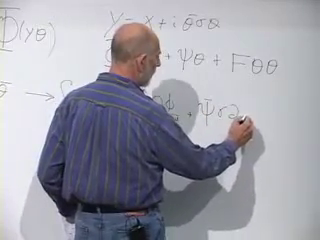
\includegraphics[width=0.76\textwidth]{lecture_09_figure_02.png}
\lectureframe{00:27:36.000}
\caption{Хиральная координата и приведенное выше компонентное разложение: скалярный, фермионный и вспомогательный члены.}
\end{figure}

\section{Что выделяет интеграл \texorpdfstring{\(d^2\theta\)}{d2-theta}}

Взаимодействия и массы возникают из голоморфной функции \(W(\Phi)\), суперпотенциала:
\begin{equation}
S_W
=
\int d^4x
\left[
\int d^2\theta\,W(\Phi)
+\mathrm{h.c.}
\right].
\label{eq:l9-superpotential-action}
\end{equation}
Хиральное выражение не имеет независимой зависимости от \(\bar\theta\), поэтому интегрирование по всем четырём нечётным координатам дало бы нуль. Интеграл \(d^2\theta\) вместо этого выделяет его компоненту \(\theta^2\).

Чтобы увидеть комбинаторику до перехода к общей функции, положим \(W(\Phi)=\Phi^n\). В
\begin{equation}
(\phi+\sqrt2\,\theta\psi+\theta^2F)^n,
\end{equation}
есть два способа получить ровно две \(\theta\). Можно выбрать один \(F\theta^2\) или выбрать два фермионных множителя.

\begin{classroomqa}\audiencequestion{Сколько членов содержат один выбранный \(F\theta^2\) и в остальном только скаляры: \(n-1\) или \(n\)? \lecturetimestamp{00:31:33}}
\lecturerresponse{Их \(n\). Любой из \(n\) множителей может дать \(F\theta^2\); оставшиеся \(n-1\) множителей дают \(\phi\). Вклад равен \(nF\phi^{n-1}\).}
\end{classroomqa}

\begin{classroomqa}\audiencequestion{Сколькими способами два множителя могут дать два фермиона? \lecturetimestamp{00:32:26}}
\lecturerresponse{Есть \(\binom n2=n(n-1)/2\) неупорядоченных выборов. Грассманово свёртывание фиксирует соответствующий член \(\psi\psi\).}
\end{classroomqa}

Итак, в используемом на лекции обозначении с подавленными коэффициентами,
\begin{equation}
\int d^2\theta\,\Phi^n+\mathrm{h.c.}
\;\leadsto\;
nF\phi^{n-1}
-\frac{n(n-1)}{2}\phi^{n-2}\psi\psi
+\mathrm{h.c.}
\label{eq:l9-power-extraction}
\end{equation}
Показанный здесь знак минус следует из стандартного нормированного разложения и грассмановых соглашений; при изменении соглашений формальные знаки могут сдвинуться.

\begin{classroomqa}\audiencequestion{Что произошло с членом \(\phi^n\), который вообще не содержит \(\theta\)? \lecturetimestamp{00:33:10}}
\lecturerresponse{Он присутствует в произведении, но \(d^2\theta\) его отбрасывает. Стрелка означает, что интегрирование выделяет коэффициент при \(\theta^2\); это не равенство полных выражений.}
\end{classroomqa}

\begin{figure}[H]
\centering
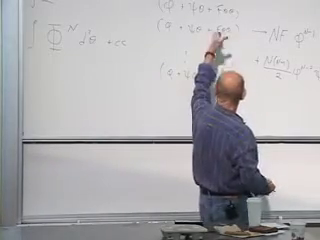
\includegraphics[width=0.82\textwidth]{lecture_09_figure_03.png}
\lectureframe{00:33:38.000}
\caption{Повторяющиеся множители суперполя и стрелка, которая выделяет, а не приравнивает, их компоненту с двумя \(\theta\).}
\end{figure}

Суммирование степеней с произвольными коэффициентами превращает комбинаторные множители в производные:
\begin{equation}
\int d^2\theta\,W(\Phi)+\mathrm{h.c.}
\;\leadsto\;
F W'(\phi)
-\frac12 W''(\phi)\psi\psi
+\mathrm{h.c.}
\label{eq:l9-W-components}
\end{equation}

\begin{classroomqa}\audiencequestion{Почему фермионный член содержит \(\phi^{n-2}\), а не \(\phi^{n-1}\)? \lecturetimestamp{00:36:32}}
\lecturerresponse{Два множителя уже дали фермионы, оставив \(n-2\) скалярных множителей. Коэффициент равен половине второй производной \(W''(\phi)\).}
\end{classroomqa}

Фермионный член важен: он даёт массу, когда \(W''\) является константой, и взаимодействие Юкавы, когда \(W''\) зависит от \(\phi\). Однако для анализа вакуума непосредственную информацию несёт вспомогательный член \(FW'\).

\section{Исключение вспомогательного поля}

Соберём члены, содержащие \(F\):
\begin{equation}
\mathcal L_F
=
F^\ast F
+F W'(\phi)
+F^\ast \overline{W'(\phi)}.
\label{eq:l9-LF}
\end{equation}
Поскольку \(\partial_\mu F\) отсутствует, полное уравнение Эйлера--Лагранжа
\begin{equation}
\partial_\mu
\frac{\partial\mathcal L}{\partial(\partial_\mu F)}
-
\frac{\partial\mathcal L}{\partial F}
=0
\end{equation}
сразу сводится к алгебраическому уравнению. Если рассматривать \(F\) и \(F^\ast\) как независимые переменные, получаем
\begin{align}
\frac{\partial\mathcal L_F}{\partial F}
&=F^\ast+W'(\phi)=0,
&
\frac{\partial\mathcal L_F}{\partial F^\ast}
&=F+\overline{W'(\phi)}=0,
\label{eq:l9-F-eom}
\end{align}
и, следовательно,
\begin{equation}
F^\ast=-W'(\phi),
\qquad
F=-\overline{W'(\phi)}.
\label{eq:l9-F-solution}
\end{equation}

\begin{figure}[H]
\centering
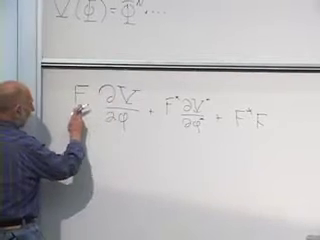
\includegraphics[width=0.82\textwidth]{lecture_09_figure_04.png}
\lectureframe{00:39:40.000}
\caption{Полное выражение для вспомогательного поля и его алгебраическое уравнение движения, видимые вместе после того, как доска оказывается незаслонённой.}
\end{figure}

\begin{classroomqa}\audiencequestion{Эту производную следует брать по \(\phi\), а не по сопряжённому полю, написанному на доске? \lecturetimestamp{00:41:21}}
\lecturerresponse{Да. Это исправление восстанавливает сопряжённую пару в уравнении~\eqref{eq:l9-F-eom}: \(F^\ast=-W'(\phi)\) и \(F=-\overline{W'(\phi)}\).}
\end{classroomqa}

Подстановка в уравнение~\eqref{eq:l9-LF} даёт
\begin{equation}
\mathcal L_F\big|_{\mathrm{on\ shell}}
=-|W'(\phi)|^2.
\end{equation}
Поскольку скалярный лагранжиан имеет вид кинетическая энергия минус потенциальная энергия, обычный скалярный потенциал равен
\begin{equation}
\boxed{V(\phi,\phi^\ast)=|W'(\phi)|^2\ge0.}
\label{eq:l9-F-potential}
\end{equation}
Этот \(V\) не является суперпотенциалом. Обозначение \(W\) мы сохраняем для голоморфной функции в суперпространстве, а \(V\) — для обычной потенциальной энергии.

\subsection{Два непосредственных примера}

При точных общепринятых нормировках,
\begin{equation}
\begin{gathered}
W(\Phi)=\frac12m\Phi^2,\\
W'(\phi)=m\phi,
\qquad V=|m|^2|\phi|^2.
\end{gathered}
\label{eq:l9-quadratic-W}
\end{equation}
Тот же член даёт массу фермиона
\(-\tfrac12m\psi\psi+\mathrm{h.c.}\), так что массы скаляра и фермиона совпадают до нарушения суперсимметрии.

Для
\begin{equation}
W(\Phi)=\frac{g}{3}\Phi^3,
\end{equation}
получаем
\begin{equation}
\begin{gathered}
W'(\phi)=g\phi^2,
\qquad V=|g|^2|\phi|^4,\\
\mathcal L_{\mathrm{Yukawa}}
=-g\phi\psi\psi+\mathrm{h.c.}
\end{gathered}
\label{eq:l9-cubic-W}
\end{equation}
Четырёхскалярная вершина описывает рассеяние двух скаляров, тогда как член Юкавы является её суперсимметричным партнёром.

\section{Два вида вакуума}

Вакуум — это постоянная конфигурация поля в минимуме \(V\); члены с производными обращаются в нуль. Поскольку выражение в уравнении~\eqref{eq:l9-F-potential} неотрицательно, возможны два случая.

\subsection{Минимум с нулевой энергией}

Если некоторое \(\phi_0\) удовлетворяет
\begin{equation}
W'(\phi_0)=0,
\end{equation}
то
\begin{equation}
V(\phi_0)=0,
\qquad
\langle F\rangle=0.
\label{eq:l9-unbroken-F}
\end{equation}
Вакуум суперсимметричен. Это аналог исчезающей намагниченности: никакая вспомогательная компонента не выделила направление в суперпространстве.

\subsection{Поднятый минимум}

Если уравнения
\begin{equation}
W'(\phi)=0
\label{eq:l9-F-flatness}
\end{equation}
не имеют в минимуме одновременного решения, то
\begin{equation}
V_{\min}>0,
\qquad
\langle F\rangle\neq0,
\label{eq:l9-broken-F}
\end{equation}
и суперсимметрия спонтанно нарушена. Действие остаётся суперсимметричным; его состояние с наименьшей энергией — нет.

\begin{figure}[H]
\centering
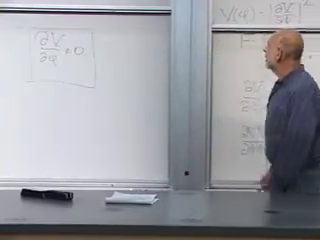
\includegraphics[width=0.88\textwidth]{lecture_09_figure_05.png}
\lectureframe{00:52:09.960}
\caption{На доске одновременно остаются положительный потенциал, уравнение для \(F\) и условие на вакуум, при этом симметричные уравнения отличены от несимметричного решения.}
\end{figure}

Утверждение о параметре порядка можно сделать точным с помощью преобразования фермиона:
\begin{equation}
\delta\psi_\alpha
=
i\sqrt2
(\sigma^\mu\bar\epsilon)_\alpha\partial_\mu\phi
+\sqrt2\,\epsilon_\alpha F.
\label{eq:l9-fermion-transformation}
\end{equation}
Для однородного вакуума член с производной исчезает. Если
\(\langle F\rangle\neq0\), суперсимметрия сдвигает фермион на ненулевую константу, так что вакуум не может быть инвариантным.\editorialnote{Уравнение~\eqref{eq:l9-fermion-transformation} — это стандартная компонентная форма, в которой явно выражено утверждение лекции о том, что компоненты суперполя преобразуются друг в друга.}

Тот же вывод следует из супералгебры. В системе покоя,
\begin{equation}
\{Q_\alpha,Q_{\dot\alpha}^\dagger\}
=2\sigma^0_{\alpha\dot\alpha}H.
\end{equation}
Взятие вакуумного среднего выражает энергию вакуума как сумму норм суперзарядов, действующих на вакуум:
\begin{equation}
E_0\ge0,
\qquad
E_0=0
\ \Longleftrightarrow\
Q_\alpha|0\rangle
=Q_{\dot\alpha}^\dagger|0\rangle=0.
\label{eq:l9-algebra-vacuum-energy}
\end{equation}
Следовательно, положительная энергия вакуума и спонтанное нарушение суперсимметрии — две стороны одного и того же утверждения о жёсткой суперсимметрии.

\begin{center}
\begin{tikzpicture}[x=1.2cm,y=1.0cm,>=Latex]
  \draw[->] (-3,0) -- (-0.2,0) node[right] {\(\phi\)};
  \draw[->] (-2.8,-0.15) -- (-2.8,2.1) node[above] {\(V\)};
  \draw[thick,teal!75!black,domain=-2.5:-0.5,samples=60]
    plot (\x,{0.65*(\x+1.5)^2});
  \fill (-1.5,0) circle (2pt);
  \node[below] at (-1.5,0) {\(F=0\)};
  \draw[->] (0.4,0) -- (3.2,0) node[right] {\(\phi\)};
  \draw[->] (0.6,-0.15) -- (0.6,2.1) node[above] {\(V\)};
  \draw[thick,orange!85!black,domain=0.9:2.9,samples=60]
    plot (\x,{0.55*(\x-1.9)^2+0.65});
  \fill (1.9,0.65) circle (2pt);
  \draw[dashed] (0.6,0.65) -- (1.9,0.65);
  \node[below] at (1.9,0.65) {\(F\neq0\)};
\end{tikzpicture}
\end{center}

\editorialnote{Минимальный пример — \(W=f\Phi\), для которого \(W'=f\) никогда не обращается в нуль и \(V=|f|^2\). Этот однополевой пример имеет плоское скалярное направление; реалистичное устойчивое нарушение по \(F\)-члену обычно реализуют с несколькими хиральными полями, как в скрытых секторах типа O'Raifeartaigh.}

\section{Что порождает нарушенная суперсимметрия}

\subsection{Расщепление масс}

Ферромагнитная аналогия теперь снова становится спектральной. Слабое внутреннее магнитное поле расщепляет атомные уровни, не лишая атом его идентичности. Аналогично, слабо передаваемый параметр порядка нарушения суперсимметрии расщепляет бозоны и фермионы, которые иначе принадлежали бы одному супермультиплету.

\begin{classroomqa}\audiencequestion{Какие частицы суперсимметрия преобразует друг в друга и потому теряют вырождение по массе, когда вакуум её нарушает? \lecturetimestamp{00:51:40}}
\lecturerresponse{Бозоны и фермионы. Их массы не обязаны оставаться равными, когда состояние больше не инвариантно относительно преобразования, которое их связывает.}
\end{classroomqa}

Расщепление не создаётся одним только \(\langle F\rangle\); оно зависит от взаимодействий, которые передают нарушение видимым полям. Если эти взаимодействия слабы, видимые частицы остаются узнаваемыми, а расщепления малы по сравнению с масштабами великого объединения или Планка. Если бы они были сильными, аналогом был бы атом, настолько искажённый огромным магнитным полем, что он превратился бы в длинный неузнаваемый объект.

\subsection{Голдстино}

Для обычного нарушенного генератора \(J|0\rangle\) даёт бозонное состояние Голдстоуна. Суперзаряд фермионен и переводит бозонные состояния в фермионные. Поскольку вакуум считается бозонным, нарушенный суперзаряд создаёт фермионное состояние с нулевой энергией:
\begin{equation}
Q_\alpha|0\rangle
\sim
|\widetilde G_\alpha,\mathbf k=0\rangle.
\label{eq:l9-goldstino}
\end{equation}
Его распространяющееся продолжение — безмассовый вейлевский фермион, голдстоуновский фермион, или голдстино.

\begin{classroomqa}
\audiencequestion{Если преобразование суперсимметрии не оставляет вакуум неизменным, какое новое состояние оно порождает? \lecturetimestamp{00:53:24}}
\lecturerresponse{Безмассовый фермион. Обычная картина теоремы Голдстоуна сохраняется, но фермионный генератор переводит бозонный вакуум в голдстино.}
\end{classroomqa}

Поэтому спонтанное нарушение жёсткой суперсимметрии имеет два неизбежных признака:
\begin{equation}
\boxed{
V_{\min}>0
\qquad\text{and}\qquad
\text{a massless goldstino}.
}
\label{eq:l9-rigid-breaking-signatures}
\end{equation}

\section{Скрытый сектор}

Удобно называть атом и ферромагнетик двумя секторами. В ферромагнетике возникает параметр порядка; атом ощущает только поле, передаваемое от него. Когда связь слаба, манипулирование атомом едва возбуждает магнон и даёт очень мало прямого доступа к магнитной среде. Тогда ферромагнетик скрыт, хотя о его присутствии судят по небольшим расщеплениям спектра.

При построении суперсимметричных моделей используется тот же язык. Дополнительные поля в скрытом секторе приобретают ненулевые средние значения \(F\)- или \(D\)-членов. Взаимодействия, называемые механизмом передачи, передают это нарушение в видимый сектор и порождают мягкие массы суперпартнёров. Слабая передача объясняет, как видимая теория может оставаться приблизительно суперсимметричной при гораздо более высоком фундаментальном масштабе, не демонстрируя при этом точного низкоэнергетического бозон--фермионного вырождения.

Построение не является автоматическим. Требуются дополнительные поля, устойчивый вакуум, в котором суперсимметрия нарушена, и контролируемый механизм передачи. Поэтому в лекции реалистическое нарушение суперсимметрии описывается как сложное и несколько искусственное, а не как единственное неизбежное следствие минимальной модели.

\section{Гравитация меняет оба признака}

\subsection{Энергия вакуума становится источником}

Без гравитации сдвиг всех энергий на константу не меняет результатов негравитационных экспериментов. При наличии гравитации плотность энергии вакуума входит в уравнение Эйнштейна как космологическая постоянная. Положительное \(V_{\min}\) вызывает ускоренное расширение. Если бы этот масштаб был сравним с масштабом физики частиц, необходимым для масс суперпартнёров, возникающая кривизна была бы неизмеримо больше наблюдаемой.

\begin{classroomqa}
\audiencequestion{Что делает с миром положительная ненулевая энергия вакуума, когда учитывается гравитация? \lecturetimestamp{01:00:40}}
\lecturerresponse{Она действует как космологическая постоянная и вызывает ускоренное расширение. При обычных масштабах физики частиц этот эффект был бы недопустимо велик.}
\end{classroomqa}

Локальная суперсимметрия, или супергравитация, изменяет формулу положительной суммы квадратов. Для ориентира стандартный потенциал \(N=1\) \(F\)-члена имеет вид
\begin{equation}
\begin{aligned}
V_F={}&e^{K/M_P^2}
\left(
K^{i\bar j}D_iW\,D_{\bar j}\overline W
-\frac{3|W|^2}{M_P^2}
\right),\\
D_iW={}&\partial_iW+\frac{\partial_iK}{M_P^2}W.
\end{aligned}
\label{eq:l9-sugra-potential}
\end{equation}
Из-за отрицательного члена положительная энергия, возникающая при нарушении суперсимметрии, в принципе может быть частично скомпенсирована. Оставшаяся часть может быть малой космологической постоянной.

\editorialnote{В лекции намеренно даётся лишь схематическая поправка, и прямо ставится под вопрос, где в формуле должна стоять масса Планка. Формула~\eqref{eq:l9-sugra-potential} даёт общепринятое выражение для хиральных мультиплетов с потенциалом Кэлера \(K\); калибровочные \(D\)-члены добавили бы ещё один неотрицательный вклад. Она не объясняет наблюдаемое крошечное значение, что и остаётся проблемой космологической постоянной.}

\subsection{Механизм супер-Хиггса}

Второй гравитационный эффект проще всего понять, подсчитав поляризации. Массивная частица со спином \(j\) имеет в системе покоя \(2j+1\) спиновых состояний.

\begin{classroomqa}
\audiencequestion{Сколько спиновых состояний имеет массивная частица со спином \(j\)? \lecturetimestamp{01:05:16}}
\lecturerresponse{\(2j+1\) спиновых состояний. В частности, массивная частица со спином один имеет три состояния, тогда как безмассовый калибровочный бозон имеет только спиральности \(+1\) и \(-1\).}
\end{classroomqa}

Различие носит кинематический характер. Массивную частицу можно лоренцевым бустом перевести в систему покоя, а затем заставить двигаться в другом направлении, сохранив ориентацию её спина, так что должны существовать все проекции. Безмассовую частицу нельзя ни обогнать, ни привести в состояние покоя. Поэтому у неё возможны только две крайние спиральности.

Для электрослабого калибровочного поля имеем
\begin{equation}
\underbrace{(+1,-1)}_{\text{massless vector}}
+
\underbrace{(0)}_{\text{Goldstone}}
\longrightarrow
\underbrace{(+1,0,-1)}_{\text{massive vector}}.
\label{eq:l9-higgs-count}
\end{equation}

\begin{classroomqa}
\audiencequestion{Откуда берётся продольная поляризация у массивного \(W\) или \(Z\)? \lecturetimestamp{01:08:50}}
\lecturerresponse{От бозона Голдстоуна. Он поглощается калибровочным полем и дополняет представление массивной частицы со спином один до трёх состояний.}
\end{classroomqa}

В гравитации есть безмассовый гравитон со спином два. Его суперсимметрический партнёр — безмассовый гравитино со спином \(\tfrac32\).

\begin{classroomqa}
\audiencequestion{Каков спин гравитона и, следовательно, его суперпартнёра? \lecturetimestamp{01:10:24}}
\lecturerresponse{У гравитона спин \(2\); спин фермионного партнёра отличается на половину и равен \(3/2\).}
\end{classroomqa}

Безмассовое гравитино имеет спиральности \(\pm\tfrac32\), тогда как массивное гравитино должно также иметь \(\pm\tfrac12\). Голдстино как раз и предоставляет эти недостающие состояния:
\begin{equation}
\begin{gathered}
\underbrace{\left(+\frac32,-\frac32\right)}_{\text{massless gravitino}}
\oplus
\underbrace{\left(+\frac12,-\frac12\right)}_{\text{goldstino}}\\
\Downarrow\\
\underbrace{\left(+\frac32,+\frac12,-\frac12,-\frac32\right)}_{\text{massive gravitino}}.
\end{gathered}
\label{eq:l9-super-higgs}
\end{equation}
Это супер-хиггсовский механизм. Как только суперсимметрия становится локальной, голдстино поглощается и больше не появляется как независимая безмассовая частица. Образовавшееся гравитино взаимодействует гравитационно, и поэтому его трудно рождать.

\section{Смена темы: почему \texorpdfstring{\(SU(5)\)}{SU(5)}?}

Теперь формализм суперсимметрии уступает место великому объединению. Калибровочная группа Стандартной модели имеет вид
\begin{equation}
G_{\mathrm{SM}}
=SU(3)_c\times SU(2)_L\times U(1)_Y.
\label{eq:l9-sm-group}
\end{equation}
Её три множителя по отдельности отвечают за цвет, слабый изоспин и слабый гиперзаряд. Вопрос объединения состоит в том, является ли это произведение сохранившейся подгруппой одной более крупной простой группы, так что кажущиеся отдельными мультиплеты частиц и калибровочные взаимодействия оказываются частями единой структуры. Минимальный кандидат, рассматриваемый здесь, — \(SU(5)\).

\subsection{Элементы группы и генераторы}

Для \(U\in SU(N)\) имеем
\begin{equation}
U^\dagger U=\mathbf1,
\qquad
\det U=1.
\label{eq:l9-SUN-def}
\end{equation}
Первое условие выражает унитарность; второе соответствует слову «special». Запишем бесконечно малый элемент в виде
\begin{equation}
U=\mathbf1+i\epsilon G+\mathcal O(\epsilon^2).
\label{eq:l9-infinitesimal-U}
\end{equation}
Унитарность требует
\begin{equation}
G^\dagger=G,
\end{equation}
а условие
\begin{equation}
\det e^{i\epsilon G}
=e^{i\epsilon\operatorname{tr}G}=1
\end{equation}
требует
\begin{equation}
\operatorname{tr}G=0.
\end{equation}
Следовательно, генераторы — это эрмитовы матрицы с нулевым следом.

Эрмитова матрица размера \(N\times N\) содержит \(N^2\) вещественных параметров: \(N\) вещественных диагональных элементов и \(N(N-1)/2\) комплексных внедиагональных элементов. Условие нулевого следа убирает один из них. Поэтому
\begin{equation}
\dim SU(N)=N^2-1,
\qquad
\dim SU(5)=24.
\label{eq:l9-SU5-dimension}
\end{equation}
Для сравнения, у \(SU(2)\) три генератора Паули, а у \(SU(3)\) — восемь цветовых генераторов.

\section{Блоки Стандартной модели внутри \texorpdfstring{\(SU(5)\)}{SU(5)}}

Разобьём пятимерное пространство на слабый двумерный блок и цветовой трёхмерный блок:
\begin{equation}
\mathbf5=\mathbf2\oplus\mathbf3.
\end{equation}
Вложенные генераторы имеют вид
\begin{align}
T^a_L
&=
\begin{pmatrix}
\tfrac12\tau^a&0\\
0&0_{3\times3}
\end{pmatrix},
&& a=1,2,3,
\label{eq:l9-SU2-block}\\
T^A_c
&=
\begin{pmatrix}
0_{2\times2}&0\\
0&\tfrac12\lambda^A
\end{pmatrix},
&& A=1,\ldots,8.
\label{eq:l9-SU3-block}
\end{align}
Матрицы Паули \(\tau^a\) порождают слабую \(SU(2)\); матрицы Гелл-Манна \(\lambda^A\) порождают цветовую \(SU(3)\). Поскольку блоки не перекрываются, эти две подгруппы коммутируют.

Ещё один диагональный генератор пропорционален единичной матрице внутри каждого блока и поэтому коммутирует с обеими. В фундаментальном представлении одна удобная конвенция для удвоенного гиперзаряда имеет вид
\begin{equation}
T_Y^{(\mathbf5)}=
\operatorname{diag}
\left(
1,1,-\frac23,-\frac23,-\frac23
\right).
\label{eq:l9-hypercharge-generator}
\end{equation}
Его след равен нулю:
\begin{equation}
1+1-3\left(\frac23\right)=0.
\end{equation}
Сопряжённое представление материи имеет противоположные собственные значения,
\begin{equation}
Y_{\overline{\mathbf5}}
=
\operatorname{diag}
\left(
-1,-1,\frac23,\frac23,\frac23
\right),
\label{eq:l9-fivebar-hypercharge}
\end{equation}
именно они и выписаны в лекции в столбце matter. Общий знак и нормировка условны; здесь используется конвенция Стандартной модели
\begin{equation}
Q=T_3+\frac{Y}{2}.
\label{eq:l9-charge}
\end{equation}
Уравнения~\eqref{eq:l9-SU2-block}--\eqref{eq:l9-hypercharge-generator} показывают
\begin{equation}
SU(3)_c\times SU(2)_L\times U(1)_Y
\subset SU(5).
\end{equation}

Три слабых генератора, восемь цветовых генераторов и один генератор гиперзаряда составляют \(12\) из \(24\) генераторов \(SU(5)\).\editorialnote{Остальные двенадцать располагаются во внедиагональных блоках \(2\times3\) и \(3\times2\). Их калибровочные бозоны переводят кваркоподобные и лептоноподобные компоненты друг в друга; в этом состоит структурный источник взаимодействий, изменяющих барионность и лептонность, которые будут рассмотрены далее.}

\begin{classroomqa}
\audiencequestion{Какие калибровочные частицы соответствуют генераторам знакомых подгрупп? \lecturetimestamp{01:31:05}}
\lecturerresponse{Восемь генераторов \(SU(3)\) дают восемь глюонов. Три генератора \(SU(2)\) дают слабые калибровочные поля, которые после электрослабого смешивания становятся \(W^\pm\) и частью \(Z\)-фотонной системы; поле \(U(1)\) даёт другую нейтральную комбинацию.}
\end{classroomqa}

\section{Одно семейство на языке левохиральных полей}

Сосредоточимся на первом поколении; та же схема повторяется для поколений мюон/чарм/стрэйндж и тау/топ/боттом. Наиболее экономно считать каждое независимое вейлевское поле левохиральным. Правохиральные частицы представляются их левохиральными зарядово-сопряжёнными полями:
\begin{equation}
Q_L=(u_L,d_L),\quad
L_L=(\nu_{eL},e_L),\quad
u^c_L,\quad d^c_L,\quad e^c_L.
\end{equation}
Их кратности таковы:
\begin{equation}
\underbrace{6}_{Q_L}
+
\underbrace{2}_{L_L}
+
\underbrace{3}_{u^c_L}
+
\underbrace{3}_{d^c_L}
+
\underbrace{1}_{e^c_L}
=15.
\label{eq:l9-fifteen-fields}
\end{equation}

\editorialnote{Минимальная Стандартная модель не содержит независимого вейлевского поля правохирального нейтрино, поэтому число полей равно \(15\). Сам по себе этот подсчёт не утверждает, что нейтрино является майорановской частицей. Добавление синглета \(\nu^c_L\) даёт \(16\) полей и естественным образом ведёт к \(SO(10)\), выходя за рамки рассматриваемой здесь конструкции \(SU(5)\).}

Пятимерный мультиплет должен помещать бесцветные компоненты слабого дублета в первые две позиции, а окрашенные слабые синглеты — в последние три.

\begin{classroomqa}
\audiencequestion{Не содержит ли предложенный столбец шесть полей, а не пять? \lecturetimestamp{01:36:14}}
\lecturerresponse{Нет. u-кварк, записанный при первом проходе, стирается. В столбец входят нейтрино, электрон и три цветовые копии анти-d-кварка: всего пять компонент.}
\end{classroomqa}

Это даёт
\begin{equation}
\overline{\mathbf5}
=
\begin{pmatrix}
\nu_{eL}\\
e_L\\
d^c_{rL}\\
d^c_{gL}\\
d^c_{bL}
\end{pmatrix}.
\label{eq:l9-fivebar}
\end{equation}
\editorialnote{В лекции это сначала просто называется пятимерным мультиплетом. В стандартных \(SU(5)\)-обозначениях, где все поля леворукие, его цветовые квантовые числа и гиперзаряд показывают, что это сопряжённое представление \(\overline{\mathbf5}\).}
Первые две компоненты преобразуются по \(SU(2)_L\), но не несут цвета. Последние три преобразуются как цветовой анти-триплет, но являются слабыми синглетами.

\begin{classroomqa}
\audiencequestion{Какие кварки несут цвет, но не имеют слабого квантового числа \(SU(2)_L\), если все поля записаны как леворукие? \lecturetimestamp{01:40:13}}
\lecturerresponse{Зарядово-сопряжённые поля праворуких кварков. Для этого пятикомпонентного мультиплета проверка заряда отбирает три поля анти-d \(d^c_{r,g,b}\).}
\end{classroomqa}

Электрические заряды в уравнении ~\eqref{eq:l9-fivebar} в сумме дают нуль:
\begin{equation}
0-1+\frac13+\frac13+\frac13=0.
\label{eq:l9-fivebar-charge-sum}
\end{equation}
Это необходимо, потому что оператор электрического заряда является бесследной комбинацией генераторов \(SU(5)\).

\begin{classroomqa}
\audiencequestion{Почему три цветовые позиции занимают анти-d-кварки, а не анти-u-кварки? \lecturetimestamp{01:43:38}}
\lecturerresponse{Нейтрино и электрон дают суммарный заряд \(-1\). Три цветовые компоненты анти-d-кварка вносят \(+1\), так что след равен нулю. Три поля анти-u дали бы неверный суммарный заряд.}
\end{classroomqa}

Остальные десять леворуких полей таковы
\begin{equation}
Q_L\;(6)
\oplus
u^c_L\;(3)
\oplus
e^c_L\;(1),
\end{equation}
и они в точности укладываются в антисимметричное представление второго ранга
\begin{equation}
\mathbf{10}\cong\wedge^2\mathbf5,
\qquad
\dim\wedge^2\mathbf5=\binom52=10.
\label{eq:l9-ten-preview}
\end{equation}
Их явное размещение — задача следующей лекции. Численное соответствие
\begin{equation}
\overline{\mathbf5}\oplus\mathbf{10}
\end{equation}
для каждого семейства Стандартной модели — первое поразительное свидетельство того, что идея \(SU(5)\) — нечто большее, чем произвольное переобозначение.

\begin{classroomqa}
\audiencequestion{Если пятёрка и десятка — разные представления, означает ли это, что их частицы не могут взаимодействовать? \lecturetimestamp{01:46:14}}
\lecturerresponse{Нет. Групповое преобразование действует внутри каждого неприводимого представления, так что оно не переводит непосредственно элемент пятёрки в элемент десятки. Тем не менее оба набора могут взаимодействовать, испуская и поглощая общие калибровочные бозоны, и взаимодействия с полем Хиггса тоже могут связывать их поля.}
\end{classroomqa}

\section{Перспектива}

Лекция проследила одну и ту же схему на очень разных масштабах. Инвариантность относительно вращений делает атомные уровни вырожденными; магнитный фон расщепляет их. Ферромагнетик создаёт такой фон, оставляя при этом лежащие в основе законы симметричными, а его бесщелевые магноны показывают, что асимметрия заключена в вакууме. В хиральной суперсимметричной теории вакуумное среднее вспомогательного поля играет роль параметра порядка:
\begin{equation}
\begin{aligned}
\langle F\rangle=0
&\quad\Longleftrightarrow\quad
\text{unbroken supersymmetry},\\
\langle F\rangle\neq0
&\quad\Longrightarrow\quad
\text{spontaneous breaking}.
\end{aligned}
\end{equation}
Нарушенный вакуум в жёсткой суперсимметрии имеет положительную энергию, расщепляет супермультиплеты и порождает голдстино. Слабая медиация мотивирует скрытый сектор; гравитация превращает энергию вакуума в космологическую проблему и поглощает голдстино в массивный гравитино.

Заключительное построение \(SU(5)\) не завершает вопрос, а ставит новый. Бесследные эрмитовы генераторы \(5\times5\) содержат блоки Стандартной модели, а первые пять полей материи в точности укладываются в \((\nu_e,e^-,d^c_r,d^c_g,d^c_b)\). Оставшиеся десять ещё предстоит поместить в антисимметричное представление. Именно с этого незавершённого сопоставления по-настоящему и начинается великое объединение.

\chapter{Мультиплеты \texorpdfstring{\(SU(5)\)}{SU(5)}, калибровочные бозоны-лептокварки и распад протона}

\lectureoverview{Великое объединение становится конкретным, когда группа Стандартной модели вкладывается в \(SU(5)\). Чтобы увидеть, что означает это утверждение, мы сначала построим необходимую теорию представлений: определяющее представление \(N\), его сопряжённое \(\overline N\), тензорные произведения, симметричные и антисимметричные тензоры и присоединённое представление. Тогда одно семейство Стандартной модели укладывается в неожиданно экономичную комбинацию \(\overline{\mathbf 5}\oplus\mathbf{10}\). Та же симметрия, которая делает эту схему красивой, также требует цветных калибровочных бозонов, превращающих кварки в лептоны. Их обмен допускает распад протона, вынуждая масштаб объединения смещаться к \(10^{15}\)--\(10^{16}\,\mathrm{GeV}\). Бегущие калибровочные константы связи указывают на сходный масштаб, а в конце мы снова вернёмся к суперсимметрии, потому что она делает их численное совпадение существенно более точным.}

\section{Почему начинать с групповых представлений?}

Существует много предложенных теорий великого объединения. Вместо их обзора мы разберём один пример и зададим три вопроса: что заставляет его работать, каких новых частиц он требует и в чём эксперимент ставит его под угрозу. Эта группа — \(SU(5)\), а её определяющая структурная особенность состоит во вложении
\begin{equation}
SU(3)_c\times SU(2)_L\times U(1)_Y
\subset SU(5).
\label{eq:l10-sm-embedding}
\end{equation}
Здесь \(SU(3)_c\) действует на цвет, \(SU(2)_L\) — на слабый изоспин, а \(U(1)_Y\) — на гиперзаряд.

Суперсимметрия не является предпосылкой этой конструкции. Ни суперсимметрия логически не влечёт великого объединения, ни великое объединение — суперсимметрии. Их связь в этой лекции численная: когда в расчёт по группе ренормализации включается спектр суперпартнёров, три калибровочные константы связи точнее сходятся к общему значению.

Частицы, которые симметрия смешивает между собой, образуют представление группы симметрии. Поэтому классификация унифицированных мультиплетов частиц сначала требует небольшой теории представлений.

\subsection{Знакомый пример \texorpdfstring{\(SU(2)\)}{SU(2)}}

Группа \(SU(2)\), связанная с обычным моментом импульса, тесно связана с вращениями трёхмерного пространства. Точнее, \(SU(2)\) является двулистным накрытием \(SO(3)\). Её неприводимые представления помечаются величиной
\begin{equation}
j=0,\frac12,1,\frac32,\ldots,
\qquad
\dim(j)=2j+1.
\label{eq:l10-su2-spins}
\end{equation}
Поэтому скаляр является синглетом, частица со спином \(\tfrac12\) — дублетом, а частица со спином один — триплетом. Слабая группа \(SU(2)_L\) представляет собой другую физическую симметрию, хотя её абстрактная теория групп та же.

\section{Определяющее представление и его сопряжённое}

Для \(SU(N)\) определяющее представление — это пространство комплексных столбцов с \(N\) компонентами,
\begin{equation}
\psi=
\begin{pmatrix}
\psi_1\\
\psi_2\\
\vdots\\
\psi_N
\end{pmatrix},
\qquad
\psi'_i=U_i{}^j\psi_j,
\qquad
U\in SU(N).
\label{eq:l10-defining}
\end{equation}
Его называют либо определяющим представлением, либо просто \(\mathbf N\). Матрицы \(U\) имеют размер \(N\times N\), а векторное пространство, на котором они действуют, имеет размерность \(N\).

Комплексное сопряжение даёт другое \(N\)-мерное представление,
\begin{equation}
\psi_i^*\longmapsto U_i{}^{j*}\psi_j^*,
\label{eq:l10-conjugate}
\end{equation}
обозначаемое как \(\overline{\mathbf N}\). При \(N>2\) определяющее и сопряжённое представления неэквивалентны. Можно поменять местами, какое из них называть представлением частицы, а какое — представлением античастицы, но, выбрав соглашение, нужно далее его сохранять.

\begin{classroomqa}
\audiencequestion{Зависит ли \(N\) в \(SU(N)\) от того, чётно \(N\) или нечётно, и относится ли оно к матрицам? \lecturetimestamp{00:07:33}}
\lecturerresponse{Здесь нет никакого ограничения по признаку чётности--нечётности. \(N\) — это размер определяющих матриц, а также размерность их определяющего представления. И \(\mathbf N\), и \(\overline{\mathbf N}\) имеют эту размерность.}
\end{classroomqa}

Античастица античастицы есть исходная частица. Вот почему перестановка названий \(\mathbf N\) и \(\overline{\mathbf N}\) меняет соглашение, а не физику.

\section{Тензорные произведения и неприводимость}

Предположим, что один объект может находиться в \(N\) внутренних состояниях и другой объект независимо может находиться в таком же числе состояний. Игнорируя положение, импульс, спин и все квантовые числа, кроме этой метки \(SU(N)\), пара имеет
\begin{equation}
N\times N=N^2
\label{eq:l10-product-count}
\end{equation}
состояний. Если первый объект находится в состоянии \(\psi_i\), а второй — в состоянии \(\phi_j\), их произведение можно записать как
\begin{equation}
\Psi_{ij}=\psi_i\phi_j,
\qquad
\Psi'_{ij}=U_i{}^kU_j{}^\ell\Psi_{k\ell}.
\label{eq:l10-tensor-transform}
\end{equation}
Это тензорное произведение \(\mathbf N\otimes\mathbf N\).

\begin{classroomqa}
\audiencequestion{Почему ответ равен \(N^2\), а не \(N^2-1\), и не нарушает ли допущение, что обе частицы имеют одну и ту же внутреннюю метку, принцип запрета Паули? \lecturetimestamp{00:10:22}}
\lecturerresponse{Эти два места здесь различимы: один объект фиксирован в одной точке, а другой — в другой. Принцип Паули накладывает ограничения на полное квантовое состояние, включая положение. Он не устраняет ни одной из этих \(N^2\) комбинаций внутренних меток. Число \(N^2-1\) появится позже из условия бесследовости в другом произведении.}
\end{classroomqa}

\(N^2\)-мерное произведение представлений, вообще говоря, приводимо. Представление приводимо, если оно содержит собственное подпространство, которое группа переводит в себя. Такие инвариантные подпространства можно отделить и рассматривать как меньшие представления; если никакого такого собственного подпространства не существует, представление неприводимо.

\subsection{Симметричные и антисимметричные тензоры}

Всякий тензор с двумя индексами единственным образом разлагается на
\begin{align}
\Psi_{ij}
&=\Psi^{(S)}_{ij}+\Psi^{(A)}_{ij},\\
\Psi^{(S)}_{ij}
&=\frac12(\Psi_{ij}+\Psi_{ji}),\\
\Psi^{(A)}_{ij}
&=\frac12(\Psi_{ij}-\Psi_{ji}).
\label{eq:l10-sym-anti}
\end{align}
Эти две части удовлетворяют условиям
\begin{equation}
\Psi^{(S)}_{ij}=\Psi^{(S)}_{ji},
\qquad
\Psi^{(A)}_{ij}=-\Psi^{(A)}_{ji}.
\end{equation}
Уравнение~\eqref{eq:l10-tensor-transform} сохраняет каждое из этих условий, поэтому групповые преобразования никогда не смешивают симметрический и антисимметрический секторы.

\editorialnote{В лекции общий подсчёт оставлен как упражнение. Размерности симметрической и антисимметрической частей равны \(N(N+1)/2\) и \(N(N-1)/2\) соответственно, а их сумма равна \(N^2\).}

\begin{figure}[htbp]
\centering
\includegraphics[width=0.78\textwidth]{lecture_10_figure_02.png}
\lectureframe{00:17:57.500}
\caption{Завершённое разложение на доске для двух состояний со спином \(\tfrac12\): три симметричных состояния и одно антисимметричное состояние.}
\label{fig:l10-spin-decomposition}
\end{figure}

Для определяющего дублета \(SU(2)\),
\begin{equation}
\mathbf2\otimes\mathbf2=\mathbf3_S\oplus\mathbf1_A.
\label{eq:l10-two-two}
\end{equation}
Если обозначить два базисных состояния как \(u\) и \(d\), то симметрический триплет имеет вид
\begin{align}
\ket{1,1}&=\ket{uu},\\
\ket{1,0}&=\frac{1}{\sqrt2}\bigl(\ket{ud}+\ket{du}\bigr),\\
\ket{1,-1}&=\ket{dd},
\end{align}
тогда как антисимметрический синглет равен
\begin{equation}
\ket{0,0}
=\frac{1}{\sqrt2}\bigl(\ket{ud}-\ket{du}\bigr).
\end{equation}
Это знакомое сложение двух спиновых угловых моментов \(\tfrac12\): четыре исходных состояния перегруппировываются в спин один и спин ноль.

\section{Частица и античастица: присоединённое представление}

Теперь объединим определяющее представление с его сопряжённым. Произведение по-прежнему имеет \(N^2\) компонент, но преобразуется как матрица:
\begin{equation}
M_i{}^j\in\mathbf N\otimes\overline{\mathbf N},
\qquad
M\longmapsto U M U^\dagger.
\label{eq:l10-matrix-transform}
\end{equation}
В отличие от \(\mathbf N\otimes\mathbf N\), между одним фундаментальным и одним антифундаментальным индексом нет осмысленной симметрии перестановки. Естественное разложение здесь вместо этого таково:
\begin{equation}
M
=
\frac{\operatorname{tr}M}{N}\,\mathbf1_N
+
\left(M-\frac{\operatorname{tr}M}{N}\,\mathbf1_N\right).
\label{eq:l10-trace-split}
\end{equation}
Первый член является синглетом, а бесследовая часть — присоединённым представлением:
\begin{equation}
\mathbf N\otimes\overline{\mathbf N}
=\mathbf1\oplus\mathbf{Adj},
\qquad
\dim\mathbf{Adj}=N^2-1.
\label{eq:l10-adjoint}
\end{equation}

\begin{figure}[htbp]
\centering
\includegraphics[width=0.67\textwidth]{lecture_10_figure_04.png}
\lectureframe{00:23:47.500}
\caption{Вывод на доске для \(\mathbf N\otimes\overline{\mathbf N}\): его \(N^2-1\) бесследовых компонент образуют присоединённое представление.}
\label{fig:l10-adjoint}
\end{figure}

Для \(SU(3)\) это даёт знакомый октет,
\begin{equation}
\mathbf3\otimes\overline{\mathbf3}
=\mathbf8\oplus\mathbf1,
\end{equation}
и 8 глюонов преобразуются по присоединённому представлению. Для \(SU(2)\) присоединённое представление имеет размерность 3 и преобразуется как спин 1.

\section{Одно семейство Стандартной модели}

Наблюдаются три поколения, но \(SU(5)\) повторяет одно и то же построение отдельно для каждого. Это не объясняет, почему существует три копии. Поэтому мы сосредоточимся на первом поколении.

Все поля будут записаны как левые вейлевские поля. Правый фермион представляется своим левым зарядово-сопряжённым полем:
\begin{equation}
u^c_L,\qquad d^c_L,\qquad e^c_L.
\label{eq:l10-left-handed-bookkeeping}
\end{equation}
Верхний индекс \(c\) обозначает зарядовое сопряжение; например, \(d^c_L\) — это левое поле анти-d-кварка с электрическим зарядом \(+\tfrac13\).

В стандартных обозначениях \(SU(5)\) пять из пятнадцати левых полей объединяются в
\begin{equation}
\overline{\mathbf5}
=
\begin{pmatrix}
\nu_{eL}\\
e_L\\
d^c_{rL}\\
d^c_{gL}\\
d^c_{bL}
\end{pmatrix}.
\label{eq:l10-fivebar}
\end{equation}
Порядок выбран так, что сначала идёт двумерный слабый блок, а затем трёхмерный цветовой блок. Слабые преобразования смешивают первые две компоненты, цветовые преобразования смешивают последние три, а внедиагональные генераторы \(SU(5)\) соединяют эти два блока.

\editorialnote{В лекции столбец в уравнении~\eqref{eq:l10-fivebar} называется \(\mathbf5\), а позднее антисимметричный мультиплет называется \(\overline{\mathbf{10}}\). Это глобально сопряжённая конвенция. Мы используем современный стандарт \(\overline{\mathbf5}\oplus\mathbf{10}\); если сопрячь каждое представление, то обозначения лекции воспроизводятся без изменения её физики.}

Полный минимальный набор полей первого поколения имеет вид
\begin{equation}
\begin{gathered}
\underbrace{Q_L=(u_L,d_L)}_{6}
\oplus
\underbrace{L_L=(\nu_{eL},e_L)}_{2},\\
\underbrace{u^c_L}_{3}
\oplus
\underbrace{d^c_L}_{3}
\oplus
\underbrace{e^c_L}_{1},\\
6+2+3+3+1=15.
\end{gathered}
\label{eq:l10-fifteen}
\end{equation}
В минимальной Стандартной модели нет независимого \(\nu^c_L\), поэтому она не даёт перенормируемой массы нейтрино. Нейтринные осцилляции показывают, что это минимальное утверждение неполно: в природе существуют малые ненулевые массы нейтрино, и требуется расширение.

\begin{classroomqa}
\audiencequestion{Когда масса фермиона переводит левое состояние в правое, превращает ли она также частицу в её античастицу? \lecturetimestamp{00:34:00}}
\lecturerresponse{Нет. Масса электрона связывает левый электрон с правым электроном того же электрического заряда. В нотации, где все поля левые, второе поле представляется как \(e^c_L\), но четырёхкомпонентная частица остаётся электроном. Только нейтральное поле может иметь майорановскую массу, которая отождествляет частицу и античастицу.}
\end{classroomqa}

\section{Калибровочные бозоны, видимые в пятёрке}

Каждому генератору калибровочной симметрии соответствует калибровочное поле. В уравнении~\eqref{eq:l10-fivebar} уже можно распознать знакомые переходы:
\begin{itemize}
\item слабые калибровочные поля действуют между \(\nu_{eL}\) и \(e_L\);
\item глюоны действуют между тремя цветами \(d^c_L\);
\item нейтральные генераторы действуют по диагонали;
\item новые недиагональные генераторы превращают лептонную компоненту в цветную или наоборот.
\end{itemize}

Глюон можно представить как несущий цветовые квантовые числа пары кварк--антикварк. В лекции используется обычная мнемоника мировых линий: проследите вылетающий антикварк назад через вершину испускания, и он будет выглядеть как кварк, движущийся вперёд. Поэтому испущенное поле несёт квантовые числа пары кварк--антикварк. На языке представлений это в точности бесследовая часть \(\mathbf3\otimes\overline{\mathbf3}\).

Для \(SU(5)\),
\begin{equation}
\dim\mathbf{Adj}_{SU(5)}=5^2-1=24.
\end{equation}
Разложение этих калибровочных полей относительно подгруппы Стандартной модели имеет вид
\begin{equation}
\mathbf{24}
=
(\mathbf8,\mathbf1)_0
\oplus(\mathbf1,\mathbf3)_0
\oplus(\mathbf1,\mathbf1)_0
\oplus(\mathbf3,\mathbf2)_{-5/6}
\oplus(\overline{\mathbf3},\mathbf2)_{5/6},
\label{eq:l10-adjoint-sm}
\end{equation}
где упорядоченная пара обозначает \(SU(3)_c\times SU(2)_L\), а нижний индекс — гиперзаряд.

\editorialnote{Уравнение~\eqref{eq:l10-adjoint-sm} явно показывает блочную структуру, изображённую в лекции. Первые три члена содержат знакомые цветовые и электрослабые калибровочные поля. Последние два члена — это двенадцать вещественных степеней свободы, которые по принятому соглашению называют бозонами \(X\) и \(Y\).}

\begin{figure}[htbp]
\centering
\begin{tikzpicture}[x=1.05cm,y=0.82cm]
  \draw[thick] (0,0) rectangle (5,5);
  \draw[thick] (2,0) -- (2,5);
  \draw[thick] (0,3) -- (5,3);
  \fill[blue!9] (0,3) rectangle (2,5);
  \fill[orange!10] (2,0) rectangle (5,3);
  \fill[teal!9] (2,3) rectangle (5,5);
  \fill[teal!9] (0,0) rectangle (2,3);
  \node[align=center] at (1,4) {weak and\\neutral fields};
  \node[align=center] at (3.5,1.5) {gluons and\\neutral field};
  \node[align=center] at (3.5,4) {\(X,Y\)};
  \node[align=center] at (1,1.5) {\(\overline X,\overline Y\)};
  \node[above] at (1,5) {\(2\)};
  \node[above] at (3.5,5) {\(3\)};
\end{tikzpicture}
\caption{Блочная структура \(2\oplus3\) калибровочного поля \(SU(5)\). Недиагональные блоки соединяют лептоны и цветные поля.}
\label{fig:l10-gauge-blocks}
\end{figure}

При \(Q=T_3+Y\) цветной слабый дублет в уравнении~\eqref{eq:l10-adjoint-sm} имеет заряды \(-\tfrac13\) и \(-\tfrac43\); его сопряжение имеет заряды \(+\tfrac13\) и \(+\tfrac43\). В лекции эти частицы называются \(X\) и \(Y\), но при этом явно не фиксируется, какое имя какому заряду соответствует. Переход и заряд составляют инвариантное содержание.

\begin{classroomqa}
\audiencequestion{Существуют ли три версии каждого нового калибровочного бозона \(X\) или \(Y\)? \lecturetimestamp{00:41:28}}
\lecturerresponse{Да. Переход соединяет цветную кварковую компоненту с бесцветной лептонной компонентой, поэтому обмениваемый бозон должен нести недостающий цвет. Поля \(X/Y\) образуют цветовые триплеты и могут испускать или поглощать глюоны.}
\end{classroomqa}

Цветные частицы не наблюдаются как изолированные асимптотические состояния. Новые калибровочные бозоны должны распадаться или адронизоваться в цветонейтральные комбинации, точно так же, как кварки.

\section{Почему мультиплет содержит антидаун-кварки}

Генераторы \(SU(N)\) — это бесследовые эрмитовы матрицы. Чтобы увидеть связь со словом «special», запишем бесконечно малый элемент группы в виде
\begin{equation}
U(\epsilon)=e^{i\epsilon T}.
\end{equation}
Унитарность даёт \(T^\dagger=T\), тогда как
\begin{equation}
1=\det U=e^{i\epsilon\operatorname{tr}T}
\end{equation}
для произвольного \(\epsilon\) даёт
\begin{equation}
\operatorname{tr}T=0.
\label{eq:l10-traceless-generator}
\end{equation}

Электрический заряд есть линейная комбинация генераторов. В столбце полей материи в уравнении ~\eqref{eq:l10-fivebar} он действует как
\begin{equation}
Q_{\overline5}
=
\operatorname{diag}
\left(0,-1,\frac13,\frac13,\frac13\right),
\qquad
\operatorname{tr}Q_{\overline5}=0.
\label{eq:l10-charge-fivebar}
\end{equation}
Следовательно,
\begin{equation}
0-1+3\left(\frac13\right)=0.
\end{equation}
При замене антидаун-полей на даун-поля получилось бы
\begin{equation}
0-1+3\left(-\frac13\right)=-2,
\end{equation}
что не может быть следом генератора \(SU(5)\). Поэтому это на первый взгляд странное приписывание антидаун-полей диктуется групповой структурой.

\section{Оставшиеся десять фермионов}

Остальные десять полей получаются из антисимметрического тензора с двумя индексами. В стандартном соглашении это антисимметрическая часть
\begin{equation}
\mathbf5\otimes\mathbf5
=\mathbf{15}_S\oplus\mathbf{10}_A.
\label{eq:l10-five-five}
\end{equation}
На лекции его строят, временно записывая сопряжённые квантовые числа
\begin{equation}
\chi=
\begin{pmatrix}
\nu^c\\
e^c\\
d_r\\
d_g\\
d_b
\end{pmatrix}.
\label{eq:l10-aux-five}
\end{equation}
Это лишь вспомогательный приём для тензорного произведения представлений, а не утверждение о том, что существует второй физический пятиплет составных частиц.

Пусть
\begin{equation}
\Psi^{ij}=-\Psi^{ji},
\qquad
i,j=1,\ldots,5.
\label{eq:l10-antisym-ten}
\end{equation}
Все диагональные элементы равны нулю, а нижнетреугольная часть определяется верхнетреугольной. Следовательно,
\begin{equation}
\dim\mathbf{10}
=\binom52
=\frac{5\cdot4}{2}
=10.
\label{eq:l10-ten-count}
\end{equation}

Электрический заряд элемента равен сумме зарядов строки и столбца в уравнении ~\eqref{eq:l10-aux-five}. Отсюда сразу получаются \(e^c\) в позиции weak--weak, даун- и ап-кварки в блоках weak--color, а анти-ап-поля в блоке color--color.

\begin{classroomqa}
\audiencequestion{Когда объединяются обозначения позитрона и даун-кварка, должен ли получающийся элемент быть бозоном \(X\)? \lecturetimestamp{00:53:08}}
\lecturerresponse{Нет. На этом этапе мы строим фермионное представление, а не адъюнктное представление калибровочных бозонов. Заряды складываются как \(1-\tfrac13=\tfrac23\), поэтому элемент имеет квантовые числа ап-кварка.}
\end{classroomqa}

Согласованный выбор цветовых знаков таков:
\begin{equation}
\Psi^{ij}=
\begin{pmatrix}
0 & e^c & d_r & d_g & d_b\\
-e^c & 0 & u_r & u_g & u_b\\
-d_r & -u_r & 0 & u_b^c & -u_g^c\\
-d_g & -u_g & -u_b^c & 0 & u_r^c\\
-d_b & -u_b & u_g^c & -u_r^c & 0
\end{pmatrix}.
\label{eq:l10-ten-matrix}
\end{equation}
Изменение фаз полей меняет некоторые выписанные знаки, но не представление и не состав частиц.

\begin{figure}[htbp]
\centering
\includegraphics[width=0.83\textwidth]{lecture_10_figure_05.png}
\lectureframe{00:59:17.500}
\caption{Ничем не загороженная \(2\oplus3\) антисимметрическая матрица материи после того, как на занятии были проверены её элементы и цветовые метки.}
\label{fig:l10-ten-board}
\end{figure}

\begin{classroomqa}
\audiencequestion{Должно ли десяти-мерное представление быть записано в виде матрицы, или его можно записать столбцом? \lecturetimestamp{00:56:24}}
\lecturerresponse{Возможны оба варианта. Можно перечислить десять независимых компонент в столбец, но антисимметрическая матрица \(5\times5\) показывает, как \(SU(5)\) действует на оба её индекса, и потому гораздо информативнее.}
\end{classroomqa}

\begin{classroomqa}
\audiencequestion{В блоке color--color элемент, помеченный как \(u\), на самом деле должен быть анти-ап-полем? \lecturetimestamp{00:57:51}}
\lecturerresponse{Да. Надпись на доске исправляется на \(u^c\), то есть на левое анти-ап-поле. Два базисных заряда даун-типа в сумме дают \(-\tfrac23\), что и есть электрический заряд анти-ап-кварка.}
\end{classroomqa}

\begin{classroomqa}
\audiencequestion{В нескольких элементах матрицы цветовые метки опущены. Сохраняется ли цвет по-прежнему? \lecturetimestamp{00:58:05}}
\lecturerresponse{Да. Три цветовых слота соответствуют красному, зелёному и синему. Метки опущены лишь для того, чтобы не загромождать запись.}
\end{classroomqa}

Антисимметричная пара цветовых фундаментальных представлений преобразуется как антицвет:
\begin{equation}
\wedge^2\mathbf3\simeq\overline{\mathbf3},
\qquad
(rg,rb,gb)\sim(\overline b,-\overline g,\overline r).
\label{eq:l10-anticolor}
\end{equation}
Именно поэтому три независимых элемента в блоке цвет--цвет образуют в точности цветовой триплет анти-up-кварка.

Одно поколение теперь собрано в виде
\begin{equation}
\overline{\mathbf5}\oplus\mathbf{10}.
\label{eq:l10-family}
\end{equation}
Поразительно, что \(u_L\) и \(u^c_L\) входят в один неприводимый мультиплет, тогда как \(d_L\) и \(d^c_L\), или \(e_L\) и \(e^c_L\), находятся в разных мультиплетах.

\begin{classroomqa}
\audiencequestion{Если калибровочные преобразования действуют только внутри каждого представления, как масса может связывать поля, лежащие в пятёрке с чертой и десятке? \lecturetimestamp{01:00:40}}
\lecturerresponse{Калибровочные бозоны не поворачивают одно неприводимое представление материи в другое. Поля Хиггса и юкавские связи могут соединять разные представления, образуя при этом в целом \(SU(5)\)-инвариантное взаимодействие; после того как поле Хиггса приобретает вакуумное среднее, эти взаимодействия порождают массы.}
\end{classroomqa}

\section{Калибровочные бозоны действуют как сдвиги}

После того как представление собрано, действие калибровочного бозона можно понимать как сдвиг между его элементами. Нейтральный бозон может оставлять метку неизменной, слабый бозон перемещает по слабым слотам, глюон — по цветовым слотам, а бозон \(X/Y\) — между слабыми и цветовыми слотами. У заряженных калибровочных бозонов есть античастицы, поэтому каждому сдвигу соответствует обратный процесс.

Для антисимметричного тензора бесконечно малое преобразование действует на любой из двух индексов:
\begin{equation}
\delta\Psi^{ij}
=
i\epsilon
\left(
T^i{}_k\Psi^{kj}
+
T^j{}_k\Psi^{ik}
\right).
\label{eq:l10-two-index-action}
\end{equation}
В матричной картине первый член сдвигает по вертикали, а второй — по горизонтали. Составные метки, использованные для построения тензора, служат лишь мнемоникой; уравнение~\eqref{eq:l10-two-index-action} — это точное группотеоретическое утверждение.

Слабые сдвиги переводят \(d\) в \(u\); это кварковый процесс, лежащий в основе бета-распада нейтрона. Цветовые сдвиги меняют красный, зелёный и синий, не меняя аромата. Внедиагональные сдвиги делают нечто новое:
\begin{equation}
\begin{aligned}
d^c&\longleftrightarrow e,
& d^c&\longleftrightarrow\nu,\\
d&\longleftrightarrow u^c,
& u&\longleftrightarrow e^c,
\end{aligned}
\label{eq:l10-leptoquark-shifts}
\end{equation}
при этом соответствующее поле \(X/Y\) несёт разность заряда и цвета.

\begin{classroomqa}
\audiencequestion{Что означают сдвиги между четвёртым и пятым слотами, и что насчёт сдвига из первого в четвёртый? \lecturetimestamp{01:10:36}}
\lecturerresponse{Сдвиг четвёртый--пятый меняет один цвет на другой и является глюонным переходом. Сдвиг первый--четвёртый пересекает границу между слабым и цветовым блоками и является одним из новых переходов с \(X/Y\).}
\end{classroomqa}

\begin{classroomqa}
\audiencequestion{Можно ли явно заполнить один элемент нижней половины антисимметричной матрицы? \lecturetimestamp{01:11:23}}
\lecturerresponse{Да. Каждый элемент нижнего треугольника равен отрицанию транспонированного элемента верхнего треугольника. Заполнение одного делает правило наглядным; заполнение всех не добавляет никаких новых состояний.}
\end{classroomqa}

\section{Опасное следствие: распад протона}

Бозон \(X/Y\) может связывать кварк с лептоном в одной вершине и два поля кваркового типа — в другой. При импульсах, значительно меньших его массы, интегрирование по тяжёлому бозону приводит к взаимодействию размерности шесть схематического вида
\begin{equation}
\mathcal L_{\mathrm{eff}}
\sim
\frac{g_5^2}{M_X^2}\,(qq)(q\ell)
+\text{h.c.}
\label{eq:l10-effective-proton}
\end{equation}
Оно по отдельности нарушает барионное и лептонное числа, сохраняя при этом комбинации, предписываемые объединённым калибровочным взаимодействием.

На доске прослеживается судьба одного d-кварка и одного u-кварка при обмене тяжёлой частицей. d-кварк превращается в позитрон, первый u-кварк — в анти-u-кварк, а второй остаётся спектатором:
\begin{equation}
uud
\longrightarrow
e^++u\overline u.
\label{eq:l10-quark-decay}
\end{equation}
Начальное состояние — протон. Пара \(u\overline u\) может адронизоваться в нейтральный пион, что даёт
\begin{equation}
p\longrightarrow e^++\pi^0.
\label{eq:l10-proton-pion}
\end{equation}

\begin{figure}[htbp]
\centering
\includegraphics[width=0.82\textwidth]{lecture_10_figure_06.png}
\lectureframe{01:16:02.500}
\caption{Завершённое построение на доске обмена тяжёлым бозоном внутри протона, со спектаторным u-кварком и видимым каналом с позитроном.}
\label{fig:l10-proton-board}
\end{figure}

В лекции также упоминается \(p\to e^++\gamma\), где пара кварк--антикварк аннигилирует электромагнитно. Этот канал испытывает дополнительное электромагнитное подавление по сравнению с прямой адронизацией.

Эта возможность — не факультативное украшение модели. Как только простая группа содержит генераторы, связывающие кварки и лептоны, в общем случае ожидаются процессы с нарушением барионного числа. Если бы они происходили на обычных временны́х масштабах слабого или электромагнитного взаимодействия, не смогли бы существовать ни ядра, ни водород, ни макроскопическое вещество.

\section{Почему протон живёт так долго?}

\begin{classroomqa}
\audiencequestion{Является ли константа связи, порождающая бозон \(X\), той же самой объединённой константой связи, которой описывается остальная часть группы? \lecturetimestamp{01:18:34}}
\lecturerresponse{На масштабе объединения — да. Простая калибровочная теория \(SU(5)\) имеет одну калибровочную константу связи \(g_5\). Низкоэнергетические сильная, слабая и гиперзарядовая константы связи различаются, потому что после нарушения объединённой симметрии они по-разному зависят от масштаба.}
\end{classroomqa}

Константу связи нельзя выбрать фантастически малой, не отказавшись от объединённой структуры. Имеющееся подавление даёт тяжёлый пропагатор:
\begin{equation}
\mathcal A
\sim
\frac{g_5^2}{M_X^2}.
\label{eq:l10-amplitude}
\end{equation}
При возведении амплитуды в квадрат появляется \(g_5^4/M_X^4\). Оценку скорости распада завершают размерностный анализ и матричный элемент протона:
\begin{equation}
\Gamma_p
\sim
C_{\mathrm{had}}\,
\frac{\alpha_5^2\,m_p^5}{M_X^4},
\qquad
\alpha_5=\frac{g_5^2}{4\pi},
\label{eq:l10-rate}
\end{equation}
где \(C_{\mathrm{had}}\) включает групповые множители, эффекты ренормировки и непертурбативный адронный матричный элемент.

\editorialnote{В лекции выделяется существенная зависимость \(g^4/M_X^4\) и отмечается, что множители массы протона опущены. Уравнение~\eqref{eq:l10-rate} восстанавливает требуемую массовую размерность, не претендуя на точный расчёт времени жизни.}

\begin{classroomqa}
\audiencequestion{Делает ли малый множитель \(g^4\), возможно порядка \(10^{-8}\) в грубой аудиторной оценке, время жизни уже достаточно долгим? \lecturetimestamp{01:25:13}}
\lecturerresponse{Нет. Он помогает, но разрыв между микроскопическим временем сильного взаимодействия и ограничением на время жизни протона охватывает гораздо больше порядков величины. Решающее подавление должна обеспечить четвёртая степень тяжёлой массы.}
\end{classroomqa}

Если бы все массы были порядка массы протона, естественной единицей времени было бы примерно время прохождения света через протон:
\begin{equation}
t_p\sim\frac{1\ \mathrm{fm}}{c}\sim10^{-23}\ \mathrm{s}.
\label{eq:l10-proton-time}
\end{equation}
Уже само существование первичных протонов показывает, что их время жизни превышает возраст Вселенной, но лабораторные поиски идут несравненно дальше. В лекции микроскопическая оценка сравнивается с приводившимся тогда экспериментальным пределом
\begin{equation}
\tau_p\gtrsim10^{33}\ \mathrm{yr}.
\label{eq:l10-lifetime-bound}
\end{equation}

Не нужно наблюдать один протон так долго. Если бы время жизни составляло \(10^{15}\) лет, образец из \(10^{15}\) протонов давал бы примерно одно событие в год. В более общем случае, если наблюдаются \(N_p\) протонов в течение времени \(T\), ожидаемое число распадов равно
\begin{equation}
\langle n\rangle\simeq\frac{N_pT}{\tau_p}.
\label{eq:l10-event-count}
\end{equation}
Детектор, содержащий примерно \(10^{33}\) протонов, — это большой бак, а не астрономический объект: сами эти протоны имеют массу порядка \(10^6\) килограммов. Наблюдение такого образца превращает огромное индивидуальное время жизни в измеримую частоту событий или в более сильную нижнюю границу.

Совмещение уравнения~\eqref{eq:l10-rate} с ограничением на время жизни приводит к значению массы лептокваркового калибровочного бозона порядка
\begin{equation}
M_X\sim10^{15}\text{--}10^{16}\ \mathrm{GeV},
\label{eq:l10-mx}
\end{equation}
причём \(10^{16}\,\mathrm{GeV}\) в лекции используется как легко запоминающийся безопасный масштаб. Это на несколько порядков величины ниже планковского масштаба и потому не является автоматически несовместимым с квантовой теорией поля.

\section{Нарушенная \texorpdfstring{\(SU(5)\)}{SU(5)}-симметрия и масштаб объединения}

Поля \(X/Y\) входят в один присоединённый мультиплет \(SU(5)\) вместе с калибровочными полями Стандартной модели. Точная ненарушенная калибровочная симметрия не позволила бы, чтобы одни её компоненты имели массы порядка \(10^{16}\,\mathrm{GeV}\), тогда как фотон и глюоны оставались бы безмассовыми. Следовательно, эта симметрия должна быть спонтанно нарушена.

\begin{classroomqa}
\audiencequestion{Если бы симметрия \(SU(5)\) была ненарушенной, были бы все её калибровочные бозоны безмассовыми? \lecturetimestamp{01:29:37}}
\lecturerresponse{Да, в рассматриваемой калибровочной теории. Калибровочная инвариантность запрещает явную общую массу. Механизм Хиггса может придать массы калибровочным бозонам, связанным с нарушенными генераторами, оставляя при этом калибровочные поля ненарушенной подгруппы безмассовыми.}
\end{classroomqa}

Электрослабый механизм Хиггса уже иллюстрирует эту структуру: он отличает фотон от \(W^\pm\) и \(Z\). Великое объединение требует отдельного параметра порядка на высоком масштабе, который отличает слабый \(2\)-блок от цветового \(3\)-блока и делает внедиагональные поля \(X/Y\) чрезвычайно тяжёлыми.

По сравнению с \(10^{16}\,\mathrm{GeV}\) даже масса слабого бозона порядка \(100\,\mathrm{GeV}\) пренебрежимо мала. Далеко выше тяжёлого порога всеми массами калибровочных бозонов можно пренебречь, и полная симметрия \(SU(5)\) становится хорошим приближением. В этом и состоит смысл масштаба объединения: не в том, что низкоэнергетический мир явно обладает \(SU(5)\), а в том, что при достаточно больших энергиях процессы становятся нечувствительными к массовым расщеплениям, вызванным нарушением симметрии.

\section{Бегущие константы связи}

Калибровочные константы связи логарифмически зависят от энергетического масштаба. Если определить
\begin{equation}
\alpha_i(\mu)=\frac{g_i^2(\mu)}{4\pi},
\end{equation}
то однопетлевая эволюция имеет вид
\begin{equation}
\alpha_i^{-1}(\mu)
=
\alpha_i^{-1}(\mu_0)
-\frac{b_i}{2\pi}
\ln\!\left(\frac{\mu}{\mu_0}\right).
\label{eq:l10-running}
\end{equation}
Коэффициенты \(b_i\) зависят от калибровочной группы и от каждой частицы, достаточно лёгкой, чтобы циркулировать в соответствующих квантовых петлях.

\editorialnote{Чтобы сравнивать гиперзаряд с неабелевыми константами связи внутри \(SU(5)\), величине \(g_1\) нужно придать стандартную для великого объединения нормировку. Именно отсюда берутся упомянутые в лекции численные группотеоретические множители.}

При лабораторных энергиях обратные величины трёх констант связи различны. В качественном порядке, приведённом в лекции, наибольшей является \(1/\alpha_1\), поскольку гиперзарядовое взаимодействие слабее всего; затем идёт \(1/\alpha_2\), а наименьшей является \(1/\alpha_3\), поскольку сильное взаимодействие наиболее сильно. Кривые при недоступных энергиях напрямую не измеряются. Их вычисляют из наблюдаемых низкоэнергетических значений, спектра частиц и петлевых диаграмм, определяющих бета-функции. При составе частиц Стандартной модели они становятся почти прямыми линиями, если строить их как функции \(\log\mu\).

\begin{figure}[htbp]
\centering
\includegraphics[width=0.74\textwidth]{lecture_10_figure_07.png}
\lectureframe{01:36:32.500}
\caption{График на доске, показывающий сближение обратных калибровочных констант связи вблизи \(10^{16}\,\mathrm{GeV}\). Обведённая область отмечает место их неидеального совпадения.}
\label{fig:l10-running-board}
\end{figure}

Ниже порога объединения симметрия нарушена, лёгкий спектр не заполняет полных вырожденных мультиплетов \(SU(5)\), и три коэффициента бета-функций различаются. Поэтому константы связи бегут с разными скоростями. На высоком масштабе спрашивают, достигают ли они общего значения:
\begin{equation}
\alpha_1(M_{\mathrm{GUT}})
\stackrel{?}{=}
\alpha_2(M_{\mathrm{GUT}})
\stackrel{?}{=}
\alpha_3(M_{\mathrm{GUT}}).
\label{eq:l10-unification-condition}
\end{equation}

Если учитывать только несуперсимметричный спектр Стандартной модели, эти линии сближаются в области \(10^{15}\)--\(10^{16}\,\mathrm{GeV}\), но расходятся на заметную величину; в лекции говорится, что согласие составляет примерно пятнадцать процентов. Важное совпадение состоит в том, что это также масштаб, требуемый стабильностью протона.

\section{Заключительный вопрос о нейтроне}

\begin{classroomqa}
\audiencequestion{Если бы спектаторный u-кварк в диаграмме распада протона был заменён на d-кварк, описывало бы это распад нейтрона, и играл бы роль бозон \(X\)? \lecturetimestamp{01:36:40}}
\lecturerresponse{Это определяло бы великообъединённый канал нейтрона, например \(n\to e^++\pi^-\), но это не привычный распад свободного нейтрона. Обычный бета-распад нейтрона — это \(n\to p+e^-+\overline\nu_e\), и он идёт за счёт слабого взаимодействия. Если бы порядок масс протон--нейтрон был обратным, бета-стабильность также обратилась бы, тогда как гораздо более медленный великообъединённый канал мог бы сохраниться.}
\end{classroomqa}

Это различие отделяет кинематику от нового взаимодействия. То, какой нуклон испытывает бета-распад, зависит от разности масс протон--нейтрон; нарушение барионного числа при обмене \(X/Y\) — отдельный, чрезвычайно подавленный механизм.

\section{Суперсимметрия и более широкая перспектива}

Добавление спектра суперсимметричных партнёров изменяет коэффициенты бета-функций в ~\eqref{eq:l10-running}. В изложении лекции три экстраполированные константы связи тогда сходятся с точностью примерно до одного процента. Это не доказывает ни суперсимметрию, ни великое объединение, но именно по этой эмпирической причине эти две идеи часто обсуждают вместе.

Мультиплеты вещества можно объединить ещё сильнее. При
\begin{equation}
SO(10)\supset SU(5),
\end{equation}
одно спинорное представление разлагается как
\begin{equation}
\mathbf{16}
\longrightarrow
\mathbf{10}\oplus\overline{\mathbf5}\oplus\mathbf1.
\label{eq:l10-so10}
\end{equation}
Синглет естественно отождествляется с левым антинейтрино или, эквивалентно, с зарядово-сопряжённым полем правого нейтрино. Тем самым все 16 полей расширенного семейства укладываются в один неприводимый мультиплет \(SO(10)\).

Эксперименты по поиску распада протона продолжают проверять эту идею, повышая нижнюю границу на время жизни, когда события не наблюдаются. Суперсимметричные великообъединённые модели не предсказывают одного универсального времени жизни протона: дополнительные тяжёлые поля и зависящие от суперпартнёров операторы могут в широких пределах менять доминирующий канал и скорость распада.

\editorialnote{В суперсимметрическом великом объединении обмен цветным триплетом Хиггса может порождать операторы размерности 5, нарушающие барионное число, в дополнение к обсуждавшемуся здесь оператору размерности 6 с обменом калибровочного бозона. Их коэффициенты сильно зависят от тяжёлого спектра, флейворной структуры и масс суперпартнёров, что объясняет предупреждение в лекции о том, что одна лишь суперсимметрия не фиксирует никакого единственного времени жизни.}

Непреходящий урок — это скорее напряжение, чем вердикт. Теория групп с поразительной экономией объединяет кварки и лептоны, бегущие константы связи намекают на общий высокий масштаб, а суперсимметрия делает этот численный намёк более отчётливым. Та же конструкция предсказывает и опасное превращение кварков в лептоны. Поэтому любой успешный вариант должен сохранять эту элегантность и в то же время обеспечивать стабильность протона в течение почти немыслимо долгого времени. В духе заключительных слов лекции: пусть все наши протоны остаются стабильными.

\end{document}